\documentclass[a4paper]{report}
\usepackage[utf8]{inputenc}
\usepackage[T1]{fontenc}
\usepackage{RJournal}
\usepackage{amsmath,amssymb,array}
\usepackage{booktabs}

%% load any required packages FOLLOWING this line
\usepackage{multirow}
\usepackage{longtable}
\usepackage[ruled,vlined,linesnumbered,noresetcount]{algorithm2e}
\newtheorem{exmp}{Example}
\newtheorem{definition}{Definition}


\begin{document}

%% do not edit, for illustration only
\sectionhead{Contributed research article}
\volume{14}
\volnumber{2}
\year{2022}
\month{June}
\setcounter{page}{26}

%% replace RJtemplate with your article
\begin{article}
 % !TeX root = RJwrapper.tex
\title{The Concordance Test, an Alternative to Kruskal-Wallis Based on the Kendall-$\tau$ Distance: An R Package}
\author{by Javier Alcaraz, Laura Anton-Sanchez and Juan Francisco Monge}

\maketitle

\abstract{
%An abstract of less than 150 words.
The Kendall rank correlation coefficient, based on the Kendall-$\tau$ distance, is used to measure the ordinal association between two measurements. In this paper, we introduce a new coefficient also based on the Kendall-$\tau$ distance, the Concordance coefficient, and a test to measure whether different samples come from the same distribution. This work also presents a new R package, \pkg{ConcordanceTest}, with the implementation of the proposed coefficient. We illustrate the use of the Concordance coefficient to measure the ordinal association between quantity and quality measures when two or more samples are considered. In this sense, the Concordance coefficient can be seen as a generalization of the Kendall rank correlation coefficient and an alternative to the non-parametric mean rank-based methods for comparing two or more samples. A comparison of the proposed Concordance coefficient and the classical Kruskal-Wallis statistic is presented through a comparison of the exact distributions of both statistics.
}

%Section title in sentence case
\section{Introduction} \label{sec:intro}

When we have a sample of observations of a given population it may be difficult to assume that they come from a certain distribution since we may not always have any type of information about the variable under study and when we do, it may not be enough to determine the type of distribution. In these cases, parametric inference is inappropriate. Moreover, this type of technique may be unsuitable should the observations not fulfill any of the basic assumptions on which they are based; normality and a large quantity of data.

Violation of the necessary assumptions in parametric statistics necessitates the use of non-parametric statistics. Non-parametric tests do not depend on the definition of a distribution function or statistical parameters such as mean, variance, etc. The use of non-parametric tests, despite being less powerful, is also adequate when there are not enough observations available, when data are non-normal data or when ordinal data are being analyzed.

Although the first steps in non-parametric statistics began earlier, it was not until the 1930s that a systematic study in this field appeared. \cite{Fisher1935} introduced the permutation test or randomization test as a simple way to compute the sampling distribution for any test statistic under the null hypothesis that does not establish any effect on all possible outcomes. Over the next two decades some of the main non-parametric tests emerged, \cite{Friedman1940,Kendall1939,Kendall1938,Kruskal1958,Kruskal1952,Wilcoxon1947,Pitman1937,Wilcoxon1945}, among others.

The main advantages of the non-parametric tests are: the data can be nonnumerical observations while they can be classified according to some criterion, they are usually  easy to calculate and do not make any hypothesis about the distribution of the population from which the samples are taken. We can also cite two drawbacks: the non-parametric tests are less precise than other statistical models and they are based on the order of the elements in the sample and this order will likely stay the same even if the numerical data change. 

There are many non-parametric tests in the literature, which can basically be classified into four categories depending on whether: it is a test to compare two or more than two related samples or a test for comparing related or unrelated samples. Examples of the most used non-parametric tests in the literature for each of these four situations are the following: the \emph{Wilcoxon signed-rank test} \citep{Wilcoxon1945} for comparing two related samples, the \emph{Mann-Whitney (Wilcoxon) test} \citep{Wilcoxon1947} for comparing two unrelated samples, the  \emph{Friedman test} \citep{Friedman1940} for comparing three or more related samples, and the \emph{Kruskal-Wallis test} \citep{Kruskal1952} for comparing three or more unrelated samples. Several methods that exploit some characteristic of the samples have appeared in the literature in recent years, such as \cite{Alhakim2008, Terpstra2003}. 

It is also possible to measure the degree of association of two variables through a non-parametric approach, in that sense we can mention the Kendall rank correlation coefficient \citep{Kendall1938} and the Spearman rank correlation coefficient \citep{Spearman1904}.

In \cite{Aparicio2020}, the  authors introduce the \emph{Kendall-$\tau$ partition ranking}; given a ranking of elements of a set and given a disjoint partition of the same set, the Kendall-$\tau$ partition ranking is the induced linear order of the subsets of the partition which follows from the given ranking of elements of a set. In this work, we propose to use the Kendall-$\tau$ distance as a concordance measure between the different samples in an ordered set of observations. In this regard, the proposed measure, which we call \emph{Concordance coefficient}, can be considered as an extension of the Kendall rank correlation coefficient when more than two samples are considered. The main difference between the proposed measure and the previous ones, is the consideration of the Kendall-$\tau$ distance instead of ranks, which use classical methods. We also propose a significance test in order to determine when more than two samples come from the same distribution, and present a comparison with the classical Kruskal-Wallis method. We illustrate the use of the proposed coefficient with a new R package, \CRANpkg{ConcordanceTest} \citep{ConcordanceTest2022}, which is freely available from the Comprehensive R Archive Network (CRAN). Actually, R establishes the state of the art in statistical software. There are currently packages for all the non-parametric tests mentioned above, for example: the \CRANpkg{Kendall} package \citep{KendallPackage2011}, which deals with the Kendall rank correlation coefficient; the \CRANpkg{pspearman} package \citep{pspearmanPackage2014}, with the Spearman rank correlation coefficient; or the \pkg{stats} package: an R Core Team and contributors' worldwide package that contains many of the non-parametric tests for comparing two or more, related or unrelated, samples. The Kendall-$\tau$ distance, on which the proposed coefficient is based, is one of the most used in distance-based models, for which there are also recent alternatives in R. See, for example, the \CRANpkg{PerMallows} \citep{Irurozki2016}, \CRANpkg{rankdist} \citep{Qian2019} or \CRANpkg{BayesMallows} packages \citep{Sorensen2020}.

The remainder of this paper is organized as follows. After a brief review in the next section of the main features of the  Kendall rank correlation coefficient and the Kruskal-Wallis statistic, in the following two sections we present the coefficient we propose in this work and illustrate its use with our \pkg{ConcordanceTest} package. Specifically, in the third section we introduce the Concordance coefficient while in the fourth section the related statistical test is presented. The fifth section includes a comparison between the Kruskal-Wallis test in the \pkg{stats} package and that presented in this work. Some final remarks follow in the last section. Appendix A presents an example of the probability distribution of the Concordance coefficient and the Kruskal-Wallis statistic. Appendix B deals with a comparison between the probability density function of the Concordance coefficient and the Kruskal-Wallis statistic for several experiments. Finally, Appendix C presents some details of how the p-values for the Concordance coefficient have been calculated and shows some critical values and exact p-values.

\section{Non-parametric tests} \label{sec:nonparametric}

This section presents the Kendall rank correlation coefficient \citep{Kendall1938}, a coefficient to measure the relationship between two samples ordinally, and the Kruskal-Wallis statistical test \citep{Kruskal1952}, which is a rank-based statistical test to measure whether different samples come from the same distribution, without assuming a given distribution for the population.

Only these two non-parametric tests are presented in detail, since the test proposed in this paper uses the Kendall-$\tau$ distance and it can be seen as an extension of the Kendall rank correlation coefficient when more than two samples are considered, and it is presented as an alternative to the Kruskal-Wallis statistical test.

The Kendall rank correlation coefficient is a non-parametric measure of correlation. This measure is based on the Kendall-$\tau$ distance between two permutations of $n$ elements. The Kendall-$\tau$ distance ($d_{K\text{-}\tau}$) is defined as the number or pairwise disagreements between two permutations $\pi_1$ and $\pi_2$. For instance, if we have three elements, the distance from permutation 123 to permutations 132, 231 and 321 is 1, 2 and 3 respectively. The maximum number of disagreements that may occur between two permutations of $n$ elements is $n(n-1)/2$ and, in this case, all the values of permutation $\pi_1$  are in the reverse order of $\pi_2$. 

The Kendall rank correlation coefficient between permutations $\pi_1$ and $\pi_2$, denoted by $\tau$, is defined by 
$$ \tau = 1 -  2 \frac{d_{K\text{-}\tau(\pi_1,\pi_2)}}{n(n-1)/2}.$$
The Kendall rank correlation  coefficient is used as a statistical test to determine whether there is a relationship or dependence between two random variables. The main advantages of this coefficient are: the data can be non-numerical observations if they can be ordered, it is easy to calculate, and the associated statistical test does not assume a known distribution of the population from which the samples are taken. 

The Kruskal-Wallis test is a non-parametric statistical method to study whether different samples come from the same population. The test is the extension of the Mann-Whitney Test \citep{Wilcoxon1947} when we have more than two samples or groups. 
The following example illustrates the Kruskal-Wallis test when comparing three samples.

\begin{exmp} \label{ex:1}
Let us assume that the effectiveness of three different treatments ($A$, $B$, $C$) has been measured for 6 individuals, two individuals being assigned to each of the treatments, with the effectiveness of each treatment being measured ordinally. We could obtain the result shown in Table~\ref{t:example}, where, for example, the effectiveness of treatment $A$ has been rated in first and third place. 
\begin{table}[h]\centering
\begin{tabular}{ccccccc}
 & $A$ & $B$ & $A$ & $C$ & $C$ & $B$ \\ \hline
 Rank & 1 & 2 & 3 & 4 & 5 & 6  \\ \hline 
 \end{tabular}
  \caption{Result for an experiment with 6 people and 3 treatments.}
  \label{t:example}
\end{table}
\end{exmp} 

The Kruskal-Wallis statistic is determined by the difference between the ranks of the individuals in each category with the average rank. In our example, the average rank of the test is $\overline{R}=3.5$, while the average rank of each of the three treatments are $\overline{R}_A=2$, $\overline{R}_B=4$ and $\overline{R}_C=4.5$. The Kruskal-Wallis statistic, denoted by $H$, is based on the calculation of the distance of each rank to the average rank, which can be expressed as follows:
$$ H =  -3(n+1)+\frac{12}{n(n+1)}\sum_{i=1}^k \frac{R_i^2}{n_i},$$
where  $n$ is the number of observations in the $k$ samples, $n_i$ is the number of observations in the $i$-th sample and $R_i$ is the sum of the ranks in the $i$-th sample. In our example, the value of the Kruskal-Wallis statistic is:
$$ H =  -3(n+1)+\frac{12}{n(n+1)}\sum_{i=1}^k \frac{R_i^2}{n_i} = -3(6+1)+\frac{12}{6(6+1)}\left (\frac{4^2}{2} + \frac{8^2}{2} + \frac{9^2}{2}  \right ) = 2. $$
Table~\ref{t:prob_KW_222} shows the probability distribution of the Kruskal-Wallis statistic for 3 treatments, each with 2 patients. Appendix A presents the Kruskal-Wallis statistic for all possible results in the experiment for 3 treatments with 2 people in each. In \cite{Spurrier2003}, the author compares different methods for approximating the null probability points. 

\begin{table}[h]	\centering\footnotesize
\begin{tabular}{cc} 
   $H$   &$ Prob$           \\ \toprule
0.00 & 0.06667 \\ \cmidrule(l){1-2}
0.29 &0.13333\\\cmidrule(l){1-2}
0.86 & 0.13333\\\cmidrule(l){1-2}
1.14 & 0.13333\\\cmidrule(l){1-2}
2.00     &  0.13333\\\cmidrule(l){1-2}
2.57 & 0.06667\\\cmidrule(l){1-2}
3.43 & 0.13333\\\cmidrule(l){1-2}
3.71 & 0.13333 \\\cmidrule(l){1-2}
4.57 & 0.06667 \\  \bottomrule[0.2mm]
\end{tabular}
\caption{Probability distribution for the Kruskal-Wallis statistic ($H$), with sample sizes $N = (2,2,2)$.}
\label{t:prob_KW_222}
\end{table}

\section{The Concordance coefficient $\tau_c$} \label{sec:CC}

In \cite{Aparicio2020}, the authors introduce the \emph{Kendall-$\tau$ partition ranking};  given a ranking of elements of a set and given a disjoint partition of the same set, the Kendall-$\tau$ partition ranking is  the induced  linear order of the subsets of the partition which follows from the given ranking of elements of a set. The Kendall-$\tau$ partition ranking presents an ordinal alternative to the mean-based ranking that uses a pseudo-cardinal scale. Let  $\pi$ be permutation of the elements of set $V$ and let $V_1$, $V_2$, $\ldots$, $V_k$ be a partition of $V$ then, the Kendall-$\tau$ distance from permutation $\pi$ is given by 
$$ d_{K\text{-}\tau} = \displaystyle \min \{ d_{K\text{-}\tau}(\rho, \pi):\text{ elements in }V_r\text{ are consecutively listed in }\rho,\,\, \forall r \}.$$

This distance is also called the  disorder of permutation $\pi$. For the calculation of the disorder of a permutation of elements, in \cite{Aparicio2020}, the authors establish that the distance or disorder of a permutation of elements
$\pi = (a|a|b|b|a|c|a|b|c|\cdots|c|a|b)$ is given by the solution of the Linear Ordering Problem (LOP) with the preference matrix $M$, where the element $m_{ab}$ of matrix $M$ indicates the number of times that an element $a$ of sample $A$ precedes an element $b$ of sample $B$ in the order $\pi$. The solution of the Linear Ordering Problem gives us a new order in the elements of $\pi$, the closest to  $\pi$, in which all the elements belonging to the same sample are listed consecutively. The book publication by \cite{Marti2011} provides an exhaustive study of the Linear Ordering Problem. 

The authors \cite{Aparicio2020} present the properties of the Kendall-$\tau$ partition ranking and compare it with classical mean and median-based rank approaches. Those properties are extracted from social choice theory and are adapted to a partition ranking, see \cite{arrow1951,Kemeny1959,zahid2015}. Two of these properties are only true for the Kendall-$\tau$ partition ranking: the \emph{Condorcet} and \emph{Deletion Independence} properties. The Condorcet property establishes that the most preferred subset must be listed before any other in any ranking; and the Deletion Independence property establishes that if any subset is removed, then the induced order of subsets does not change. In permutation $\pi=(c|c|c|b|b|a|a|c|c)$ the set $C$ is a condorcet winner, the most preferred set, but $B$ has a lesser mean rank value than set $C$ if set $A$ is not considered in the comparison; therefore, the permutation $\pi=(c|c|c|b|b|a|a|c|c)$ gives an example where ranking subsets from ranks is not very reliable. 

From \cite{Aparicio2020}, the maximum number of disagreements that may occur in a permutation of $n$ elements (where the elements are classified in $k$ subsets $V_1, V_2,\ldots, V_k$ of sizes $n_1, n_2,\ldots, n_k$ respectively) is $\sum_{r=1}^k\sum_{s =r+1}^k n_r \, n_s - (GP_{b} +\sum_{r=1}^k\sum_{s =r+1}^k \displaystyle\lfloor\frac{n_r n_s}{2}\displaystyle\rfloor )$, where $GP_{b}$ is the Generalized Pentagonal Number of $b$, and $b$ the number of subsets $V_k$ with odd cardinality.   The Generalized Pentagonal number $GP_{b}$, for $b\in \mathbb{N}$, is 
$$GP_b=\left\{ \begin{array}{ll}\displaystyle\frac{\ell(3\ell -1)}{2} & b=2\ell \,\, (b \,\, \text{even}),\\  & \\\displaystyle\frac{\ell(3\ell +1)}{2} & b=2\ell +1 \,\, (b \,\, \text{odd}).\\ \end{array} \right. $$
This maximum number of  disagreements (the maximum disorder) in a permutation $\pi$ of elements, allows us to define a relative disorder coefficient of permutation $\pi$ as
$$ relative\,  disorder(\pi) = \frac{\displaystyle d_{K\text{-}\tau}(\pi)}{\displaystyle\sum_{r=1}^k\sum_{s =r+1}^k  n_r \, n_s   -  (GP_{b} +\sum_{r=1}^k\sum_{s =r+1}^k\displaystyle\lfloor\frac{n_r n_s}{2}\displaystyle\rfloor )}.$$

\begin{definition}
	We define the  Concordance coefficient ($\tau_c$) of permutation $\pi$ as
	$$\tau_c= 1- relative\, disorder(\pi) = 1- \frac{\displaystyle d_{K\text{-}\tau}(\pi)}{\displaystyle\sum_{r=1}^k\sum_{s =r+1}^k  n_r \, n_s   -  (GP_{b} +\sum_{r=1}^k\sum_{s =r+1}^k\displaystyle\lfloor\frac{n_r n_s}{2}\displaystyle\rfloor )} .$$
\end{definition}

The  Concordance coefficient ($\tau_c$) provides a measure of independence in the $k$ samples, where $\tau_c$ is a value between 0 and 1, taking the value of 1 when there is a total order between the samples, and 0 when the disorder is maximum. In this sense, the Concordance coefficient can be seen as a generalization of the Kendall rank correlation coefficient when we have more than two samples. Given that the Concordance coefficient satisfies the properties mentioned above, we consider it is more appropriate for measuring differences between samples than a rank-based method, such as Kruskal-Wallis'.

\setcounter{exmp}{0}
\begin{exmp}[Cont.] 
Continuing with the data in Example~\ref{ex:1}, the results of the experiment provide the following order or permutation of the treatments $\pi=(a|b|a|c|c|b|)$.
\end{exmp} 

Given the order of individuals $\pi=(a|b|a|c|c|b|)$, the ordering between individuals that leaves individuals with the same treatment together is ordination ($a$ $a$ $b$ $b$ $c$ $c$) or ($a$ $a$ $c$ $c$ $b$ $b$). Both ordinations only need 3 pairwise disagreements from the permutation $\pi$. In order to find the permutation of elements (equal elements listed consecutively) closer to a given permutation, it is sufficient to solve the Linear Ordering Problem (LOP) with the preference matrix defined above. In this example, said matrix is:

\setlength{\tabcolsep}{1mm}
\begin{center}
\begin{tabular}{cccc}
&\,\,\, \,\, $A$ & $B$ & $C$\,\,\,\, \\ 
$A$&\multirow{3}{*}{  $ \left(\begin{array}{r}  $--$ \\1  \\  0 \end{array}\right.$}  &\multirow{3}{*}{  $ \begin{array}{c}3   \\ $--$  \\  2\end{array}$}   &\multirow{3}{*}{  $ \left.\begin{array}{c}4   \\2  \\  $--$ \end{array}\right)$}  \\
$B$&&&\\
$C$&&&\\
 \end{tabular},\end{center}
 
where each element of the matrix $m_{ij}$ represents the number of times an individual of a treatment $i$ precedes an individual of the treatment $j$. The solution of the LOP is the permutation of treatments which maximizes the preferences of order in the experiment, that is, in this example, the permutations of treatments $(A\ B\ C)$ or $(A\ C\ B)$ retain 9 preferences expressed in the order of individuals represented by the permutation $\pi$. Therefore, the distance of the permutation $\pi$ to a total order between treatments is $\sum_{i<j} n_i n_j -9 =3$. This distance, which is the number of pairwise disagreements needed in a permutation of elements to reach a permutation that establishes a total order between treatments, is denominated the disorder of a permutation by the authors of the work by \cite{Aparicio2020}\footnote{If the number of samples is small, we can evaluate all the possibilities in order to obtain the solution of the Linear Ordering Problem, for example, if we have 3 samples the number of feasible solutions for the LOP is $3!=6$.}.

Then, the relative  disorder of permutation $\pi$ can be evaluated as 
$$ relative \,disorder(\pi) = \frac{\displaystyle d_{K\text{-}\tau}(\pi)}{\displaystyle\sum_{r=1}^k\sum_{s =r+1}^k  n_r \, n_s   -  (GP_{b} +\sum_{r=1}^k\sum_{s =r+1}^k\displaystyle\lfloor\frac{n_r n_s}{2}\displaystyle\rfloor )} =\frac{\displaystyle 3}{\displaystyle 12  -  (0
+6  )} = \frac{3}{6}=\frac{1}{2},$$
and the Concordance coefficient
$$\tau_c= 1- relative\,disorder(\pi) = 1-\frac{1}{2}=\frac{1}{2}.$$ 
Notice that no set of this example has odd cardinality, therefore the pentagonal number is $GP_0=0$.

Table~\ref{t:prob_DK_222} shows the probability distribution of the disorder and the Concordance coefficient for 3 treatments with 2 patients each. Appendix A presents the disorder and the Concordance coefficient for all possible results in the experiment with sample sizes $N = (2,2,2)$. Figure~\ref{fig:distprob_222} compares the probability distribution of the Concordance coefficient and the Kruskal-Wallis statistic, for 3 treatments and 2 people in each treatment. Notice that some Kruskal-Wallis statistic values ($H$=2.57) are less probable than large ones. 

\begin{table}[h] 	\centering\footnotesize
\begin{tabular}{ccc} 
    $dis$ & $\tau_c$   &$ Prob$           \\ \toprule
6	&	0.0000	&	0.06667\\ \cmidrule(l){1-3}
5	&	0.1667	&	0.13333	\\ \cmidrule(l){1-3}
4	&	0.3333	&	0.20000 	\\ \cmidrule(l){1-3}
3	&	0.5000	&	0.20000\\ \cmidrule(l){1-3}
2	&	0.6667	&	0.20000	\\ \cmidrule(l){1-3}
1	&	0.8333	&	0.13333	\\ \cmidrule(l){1-3}
0	&	1.0000	&	0.06667	\\ \bottomrule[0.2mm]
\end{tabular}
\caption{Probability distribution of the disorder ($dis$) and the Concordance coefficient ($\tau_c$), with sample sizes $N = (2,2,2)$.}
\label{t:prob_DK_222}
\end{table}

\begin{figure}[h]
\centering
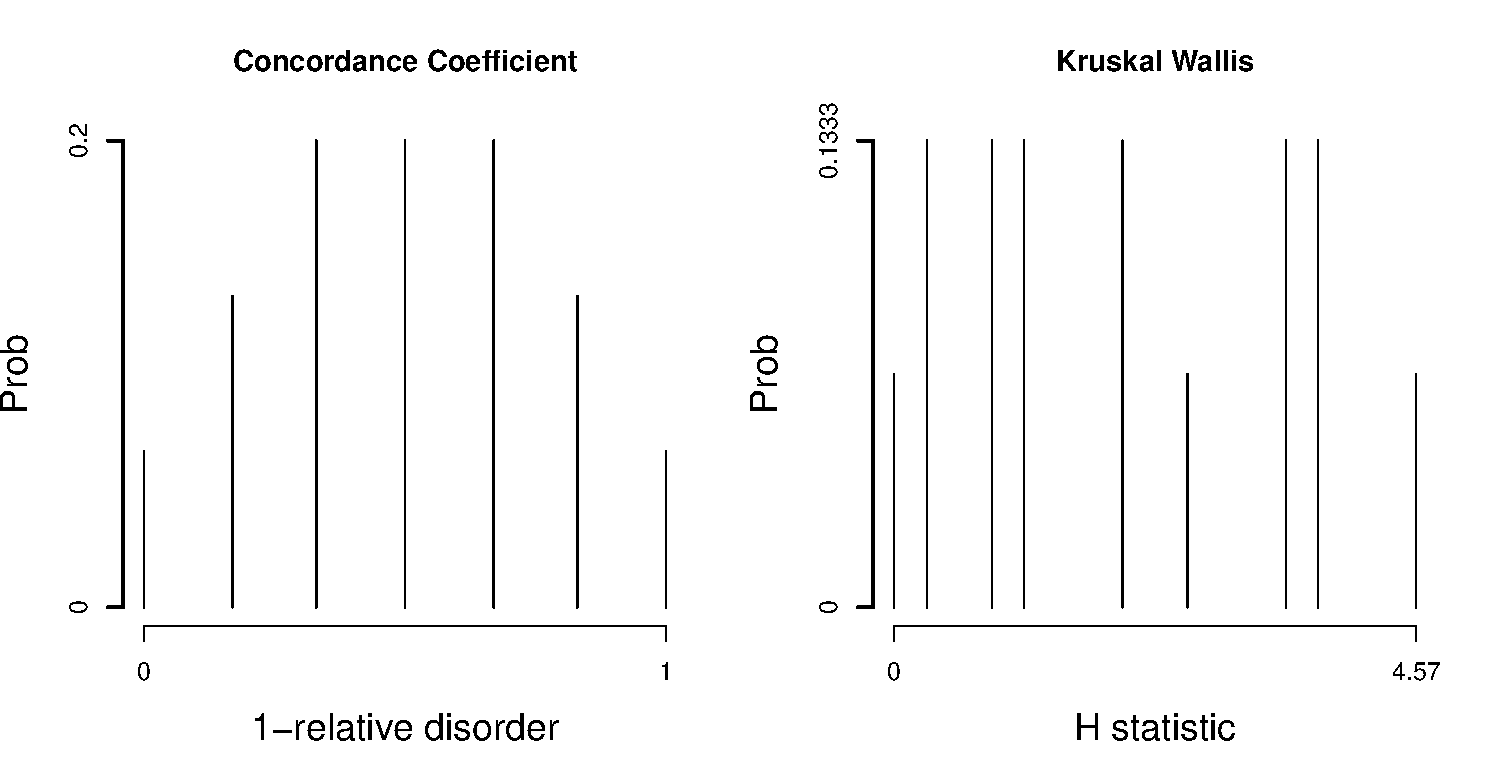
\includegraphics[width=10cm]{CC_H_222.pdf}
\caption{\label{fig:distprob_222} Probability distribution of the Concordance coefficient ($\tau_c$=1-relative disorder) and the Kruskal-Wallis statistic ($H$), with sample sizes $N = (2,2,2)$.}
\end{figure}

\subsection{The Concordance coefficient in \pkg{ConcordanceTest} package}

The R package we have developed allows to calculate both the Concordance coefficient and the Kruskal-Wallis statistic in order to facilitate their comparison. Given the high combinatorial degree of the problem of ordering samples of populations, some of the functions implemented in the package can perform the calculations exactly, exploring the entire sample space or possibilities, or they can approximate the sample space or possibilities by simulation.

The  \pkg{ConcordanceTest} package can be installed from CRAN:

\begin{example}
install.packages("ConcordanceTest")
library("ConcordanceTest")
\end{example}

and its functions can perform the calculations related only to the Concordance coefficient (default option, specified with the parameter \code{H}=0) or do them also for the Kruskal-Wallis statistic (\code{H}=1), allowing their comparison. 

To obtain the probability distribution of the statistics, it is necessary to have the set of all possible permutations that can occur in the result of the experiment that we want to analyze (90=6!/2!2!2! in Example~\ref{ex:1}). This can be obtained through the function \code{Permutations\_With\_Repetition()}, which has been developed and included in the \pkg{ConcordanceTest} package. 


The function \code{CT\_Distribution()} calculates the probability distribution of the Concordance coefficient and the Kruskal-Wallis statistic. The set of possibilities (sample space) grows very quickly with the number of elements and with the number of sets and, in some cases, to calculate the probability distribution in an exact way becomes unaffordable, making it necessary to approximate calculations. Both an exact and an approximate calculation (default option) can be done using the function \code{CT\_Distribution()}. It is used as follows:
\begin{example}
CT_Distribution(Sample_Sizes, Num_Sim = 10000, H = 0, verbose = TRUE)
\end{example}
where \code{Sample\_Sizes} is a numeric vector $(n_1,\ldots,n_k)$ containing the number of repetitions of each element, i.e., the size of each sample in the experiment. \code{Num\_Sim} is the number of simulations to be performed in order to obtain the probability distribution of the statistics (10,000 by default). If \code{Num\_Sim} is set to 0, the probability distribution tables are obtained exactly using the function \code{Permutations\_With\_Repetition()}. \code{H} is the parameter specifying whether the calculations must also be performed for the Kruskal-Wallis statistic, and \code{verbose} is a logical parameter that indicates whether some progress report of the simulations should be given.


\setcounter{exmp}{0}
\begin{exmp}[Cont.] 
Using the function \code{CT\_Distribution()} with \code{Num\_Sim} equal to 0, we could obtain the probability distribution of the Kruskal-Wallis statistic and the Concordance coefficient in Example~\ref{ex:1} (Tables~\ref{t:prob_KW_222} and \ref{t:prob_DK_222}, respectively) in an exact way. As shown in this example, we can also approximate the probability distributions of Example~\ref{ex:1} by simulating, for example, 25,000 permutations of 3 treatments with 2 patients each. Note that, for reproducibility, we always initialize the generator for pseudo-random numbers when the results rely on simulation.
\end{exmp} 
 
\begin{example}
set.seed(12)
Sample_Sizes <- c(2,2,2)
CT_Distribution(Sample_Sizes, Num_Sim = 25000, H = 1)

$C_freq
     disorder  Concordance coefficient Frequency Probability
[1,]        6                     0.00         6      0.0667
[2,]        5                     0.17        12      0.1333
[3,]        4                     0.33        18      0.2000
[4,]        3                     0.50        18      0.2000
[5,]        2                     0.67        18      0.2000
[6,]        1                     0.83        12      0.1333
[7,]        0                     1.00         6      0.0667

$H_freq
      H Statistic Frequency Probability
 [1,]        0.00         6      0.0667
 [2,]        0.29        12      0.1333
 [3,]        0.86        12      0.1333
 [4,]        1.14        12      0.1333
 [5,]        2.00        12      0.1333
 [6,]        2.57         6      0.0667
 [7,]        3.43        12      0.1333
 [8,]        3.71        12      0.1333
 [9,]        4.57         6      0.0667
\end{example}

The function \code{CT\_Distribution()} returns two elements. \code{C\_freq} is a matrix with the probability distribution of the Concordance coefficient. Each row in the matrix contains the disorder, the value of the Concordance coefficient $\tau_c$, the frequency and its probability.  \code{H\_freq} (only returned if \code{H} = 1) is a matrix with the probability distribution of the Kruskal-Wallis statistic. Each row in the matrix contains the value of the statistic $H$, the frequency and its probability. The results obtained by the function \code{CT\_Distribution()} are the same as those previously shown in Table~\ref{t:prob_DK_222} and Table~\ref{t:prob_KW_222} of Example~\ref{ex:1}.

\section{Concordance test} \label{sec:ConcordanceTest}

In this section, we present the Concordance test in order to evaluate when  different samples come from the same population distribution. The randomization test introduced by \cite{Fisher1935} establishes a framework for the statistical test based on permutations, see also \cite{Box1980,Stern1990,Welch1990}.  

If all the samples come from the same distribution, then all possible ways to rank $n$ observations divided into $k$ samples have the same probability of occurring. If a result of the experiment provides an order of the observations with a high disorder, it will support the idea that all observations come from the same population. On the contrary, a result with a small disorder will go against the claim that the observations come from the same population. In this way, we propose to consider samples that come from the same distribution as null hypothesis, while the alternative hypothesis is that some of the samples come from a different distribution.

\begin{description}
\item[$H_0$:] There is no difference among the $k$ populations.
\item[$H_a$:]  At least one of the populations differs from the other populations. 
\end{description}

The decision rule is to reject the null hypothesis if the disorder in the permutation of observations is small, equivalently if the Concordance coefficient $\tau_c$ is close to one. We reject the null hypothesis $H_0$ at the significance level $\alpha$ if $\tau_c$ is greater than the percentile $(1-\alpha)\%$ of the probability distribution of $\tau_c$. 

The following example illustrates the use of the Concordance test proposed in this work and compares it with the classical Kruskal-Wallis non-parametric test. The comparison will be made first considering that there are no ties and then modifying the data in the example so that ties appear.

\begin{exmp} \label{ex:18patients} Suppose we have applied three treatments to 18 patients, measuring the number of hours it takes these patients to recover. The results are shown in Table~\ref{t:example2}. \\

\begin{table}[h] \centering
\begin{tabular}{ccccccccccccc} \toprule
 & \multicolumn{10}{c}{Hours}\\ \hline
Treatment A & 12 & 13 & 15 & 20& 23 & 28 & 30 & 32 & 40 & 48 \\ \hline
Treatment B & 29& 31& 49 & 52 & 54 & & & & & \\ \hline
Treatment C & 24 & 26 & 44 & & & & & & &\\ \bottomrule[0.2mm]
\end{tabular}
 \caption{Result for an experiment with 18 patients and 3 treatments.}
  \label{t:example2}
\end{table}
\end{exmp}

\subsubsection{Concordance test:}

The experiment ranks the patients in the following ranking $$ (a\ a\ a\ a\ a\ c\ c\ a\ b\ a\ b\ a\ a\ c\ a\ b\ b\ b).$$

If we perform the contrast using the disorder statistic or the Concordance coefficient $\tau_c$, we must calculate the permutation of treatments that maximizes the order between patients obtained in the experiment. The matrix of preferences between treatments observed is as follows:

\begin{center}	\begin{tabular}{cccc}
		&\,\,\, \,\, $A$ & $B$ & $C$\,\,\,\, \\ 
		$A$&\multirow{3}{*}{  $ \left(\begin{array}{r}  $--$ \\7 \\  11 \end{array}\right.$}  &\multirow{3}{*}{  $ \begin{array}{c}43   \\ $--$  \\  13\end{array}$}   &\multirow{3}{*}{  $ \left.\begin{array}{c}19   \\2  \\  $--$ \end{array}\right)$}  \\
		$B$&&&\\
		$C$&&&\\
	\end{tabular}\end{center}

The order between treatments that maximizes the order between patients corresponds to the order $(A\ C\ B)$, satisfying 75 of the 95 preferences contained in the matrix, where the value 75 is the solution of the Linear Ordering Problem (LOP)\footnote{The solution of LOP for this example is the permutation of sets that maximizes the preferences in the preference  matrix. It is sufficient to compare the 6 possibilities, $(A\ B\ C) = 64 $, $(A\ C\ B) = 75 $, $(B\ A\ C) = 28$, $(B\ C\ A) = 20$, $(C\ A\ B) = 67$ and $(C\ B\ A) = 31$. }. 
 Therefore, exactly 20 = 95-75 is the number of pairwise disagreements necessary to order the samples and obtain the order (ACB), that is, the disorder is 20. The greatest disorder that an order of elements can have with samples of 10, 5 and 3 elements is given by:
 $\sum_{r=1}^3\sum_{s =r+1}^3 n_r \, n_s - (GP_{b} +\sum_{r=1}^3\sum_{s =r+1}^3 \displaystyle\lfloor\frac{n_r n_s}{2}\displaystyle\rfloor ) = 95 - (1 + 47) = 47 $, 
therefore the Concordance coefficient is $\tau_c = 1-20/47= 0.574$. The p-value of the disorder 20 or, equivalently, of the Concordance coefficient $\tau_c=0.574$ is 0.049272\footnote{Tables of p-values for the Concordance coefficient $\tau_c$ are in Appendix C.},  therefore, at a level of significance less than 5\% we can reject the null hypothesis of equality in treatments. 

\subsubsection{Kruskal-Wallis test:}

The treatments A, B and C have average ranks of 7.3, 14.2 and 9, respectively, and the sum of ranks are $R_A=73$, $R_B=71$ and $R_C=27$. 

The Kruskal-Wallis statistic is given by:
$$H = -3(n+1)+\frac{12}{n(n+1)}\sum \frac{R_i^2}{n_i}= -3(18+1)+\frac{12}{18(18+1)}\left( \frac{73^2}{10} +\frac{71^2}{5}+\frac{27^2}{3}\right)=5.6$$

In \cite{Meyer2015}, exact values for the Kruskal-Wallis contrast at different levels of significance are found. We can conclude by looking at the tables that the p-value of the $H$ statistic is greater than 0.05, therefore, we cannot reject the null hypothesis that the treatments are equally effective.

Comparing both methods, the Concordance and Kruskal-Wallis tests provide similar results about the statistic but the conclusion differs. 


\begin{exmp} \label{ex:3} Suppose we have the same experiment as in Example~\ref{ex:18patients} but with ties. The results are shown in Table~\ref{t:example3}. Ties are in bold.\\

\begin{table}[h] \centering
\begin{tabular}{ccccccccccccc} \toprule
 & \multicolumn{10}{c}{Hours}\\ \hline
Treatment A & 12 & 13 & 15 & 20& {\bf 24} & {\bf 29} & 30 & 32 & 40 & {\bf 49} \\ \hline
Treatment B & {\bf 29}& 31& {\bf 49} & 52 & 54 & & & & & \\ \hline
Treatment C & {\bf 24} & 26 & 44 & & & & & & &\\ \bottomrule[0.2mm]
\end{tabular}
 \caption{Result for an experiment with 18 patients and 3 treatments. Example with ties.}
  \label{t:example3}
\end{table}
\end{exmp}


\subsubsection{Concordance test with ties:}

The results of the experiment order the individuals according to the sequence: 
$$ (a\ a\ a\ a\ (a\ c)\ c\ (a\ b)\ a\ b\ a\ a\ c\ (a\ b)\ b\ b) $$
where the elements grouped in the order indicates that they tie. There are $8$ different possibilities in order to undo ties in the ranking of elements. If the same probability is assumed for all of them, the expected preference matrix between treatments is given distributing the preference in the comparison of repeated observations with the same weight, that is, assigning the value 0.5 to each of the treatments when two tied units are compared. The preference matrix for this example would be as follows:

\begin{center}	\begin{tabular}{cccc}
		&\,\,\, \,\, $A$ & $B$ & $C$\,\,\,\, \\ 
		$A$&\multirow{3}{*}{  $ \left(\begin{array}{r}  $--$ \\8 \\  11.5 \end{array}\right.$}  &\multirow{3}{*}{  $ \begin{array}{c}42   \\ $--$  \\  13\end{array}$}   &\multirow{3}{*}{  $ \left.\begin{array}{c}18.5   \\2  \\  $--$ \end{array}\right)$}  \\
		$B$&&&\\
		$C$&&&\\
	\end{tabular}\end{center}
	
Note that the previous matrix represents the matrix of expected preferences if all permutations of items with ties in which they are undone are considered, with the same probability of tie between elements.

The order between treatments that maximizes the order between patients, corresponds to the order $(A\ C\ B)$, satisfying 73.5 of the 95 preferences contained in the matrix, where 73.5 is the solution of the Linear Ordering Problem. Therefore, 21.5 = 95-73.5 is the expected number of pairwise disagreements necessary to order the samples and obtain the order $(A\ C\ B)$, that is, the disorder is 21.5 or, equivalently, the Concordance coefficient is $\tau = 1-21.5/47= 0.543 $, a value with a significance greater than 0.05, $p - value > 0.05$.  In this case, the observed data do not show significant evidence 
in favor of a difference in the effectiveness of treatments.

\subsubsection{Kruskal-Wallis test with ties:}

The treatments A, B and C have average ranks of 7.45, 14 and 8.83, respectively, and the sum of ranks are $R_A=74.5$, $R_B=70$ and $R_C=26.5$.

The Kruskal-Wallis statistic is given by:
$$H = -3(n+1)+\frac{12}{n(n+1)}\sum \frac{R_i^2}{n_i}= -3(18+1)+\frac{12}{18(18+1)}\left( \frac{74.5^2}{10} +\frac{70^2}{5}+\frac{26.5^2}{3}\right)=5.074$$

If we make the adjustment in the statistic for ties, we get:
$$\tilde{H} = \frac{H}{\displaystyle 1-\frac{ \sum_(t_i^3-t_i)}{N^3-N}} = \frac{5.074}{\displaystyle 1-\frac{(2^3-2)+(2^3-2)+(2^3-2)}{18^3-18}}=\displaystyle 5.0897$$

where $t_i$ is the number of ties of each value.
 
In this case, the Kruskal-Wallis test provides the same conclusion as the Concordance test; uncertainty being greater when we have ties. 

\subsection{Concordance test in \pkg{ConcordanceTest} package}

The  \pkg{ConcordanceTest} R-package  allows to perform the hypothesis test for testing whether samples originate from the same distribution with the function \code{CT\_Hypothesis\_Test()}, which carries out  the calculations by simulation. It is used as follows:
\begin{example}
CT_Hypothesis_Test(Sample_List, Num_Sim = 10000, H = 0, verbose = TRUE)
\end{example}
where \code{Sample\_List} is a list of numeric data vectors with the elements of each sample, \code{Num\_Sim} is the number of used simulations (10,000 by default), \code{H} specifies whether the Kruskal-Wallis test must also be done, and \code{verbose} is a logical parameter that indicates whether some progress report of the simulations should be given.

\setcounter{exmp}{1}
\begin{exmp}[Cont.] 
We use the \pkg{ConcordanceTest} package to perform the Concordance and Kruskal-Wallis tests of Example~\ref{ex:18patients}. We use 25,000 simulations.
\end{exmp} 
%
\begin{example}
set.seed(12)
A <- c(12,13,15,20,23,28,30,32,40,48)
B <- c(29,31,49,52,54)
C <- c(24,26,44)
Sample_List <- list(A, B, C)
CT_Hypothesis_Test(Sample_List, Num_Sim = 25000, H = 1)

$results
                        Statistic p-value
Concordance coefficient     0.574 0.04928
Kruskal Wallis              5.600 0.05292

$C_p_value
[1] 0.04928

$H_p_value
[1] 0.05292
\end{example}

The function \code{CT\_Hypothesis\_Test()} provides the value of the statistics together with the p-value associated with each of them. The result of the Kruskal-Wallis test is only returned if \code{H} = 1. Note that the approximated p-values obtained by simulation are close to the exact ones, 0.04927 and 0.05223 for the Concordance coefficient and the Kruskal-Wallis statistic, respectively. 

An alternative to the contrast performed with the function \code{CT\_Hypothesis\_Test()} is to obtain the critical values of our contrast. This can be done with the \pkg{ConcordanceTest} package both in an exact or approximate way, using the function \code{CT\_Critical\_Values()}. It is used as follows:
\begin{example}
CT_Critical_Values(Sample_Sizes, Num_Sim = 10000, H = 0, verbose = TRUE)
\end{example}
where \code{Sample\_Sizes} is a numeric vector $(n_1,\ldots,n_k)$ containing the number of repetitions of each element, i.e., the size of each sample in the experiment. \code{Num\_Sim} is the number of simulations carried out in order to obtain the probability distribution of the statistics (10,000 by default). If \code{Num\_Sim} is set to 0, the critical values are obtained in an exact way. Otherwise they are obtained by simulation. \code{H} is the parameter specifying whether the critical values of the Kruskal-Wallis test must be calculated and returned, and \code{verbose} is a logical parameter that indicates whether some progress report of the simulations should be given.

The function returns a list with two elements. \code{C\_results} are the critical values and p-values for a desired significance levels of 0.1, .05 and .01 of the Concordance coefficient, and \code{H\_results} are the critical values and p-values of the Kruskal-Wallis statistic (only returned if H = 1). 

\setcounter{exmp}{1}
\begin{exmp}[Cont.] 
We show the results of the function \code{CT\_Critical\_Values()} with sample sizes $N=(10,5,3)$ and 25,000 simulations. The results allow us to compare the test statistics with different significance levels.
\end{exmp} 

\begin{example}
set.seed(12)
Sample_Sizes <- c(10,5,3)
CT_Critical_Values(Sample_Sizes, Num_Sim = 25000, H = 1)

$C_results
              |  disorder |  Concordance coefficient |  p-value
Sig level .10          23                       0.51     0.0954
Sig level .05          20                       0.57     0.0492
Sig level .01          14                       0.70     0.0096

$H_results
              |  H Statistic |  p-value
Sig level .10           4.55     0.0995
Sig level .05           5.72     0.0497
Sig level .01           7.78     0.0097
\end{example}

To obtain the Concordance coefficient and the Kruskal-Wallis statistic from the result of an experiment, the \pkg{ConcordanceTest} package has the function \code{CT\_Coefficient()}. This function is useful when we only want to obtain the value of the statistic to check its significance using statistical tables. The function \code{CT\_Coefficient()} is used as follows:
\begin{example}
CT_Coefficient(Sample_List, H = 0)
\end{example}
where \code{Sample\_List} is a list of numeric data vectors with the elements of each sample, and \code{H} is defined as usual.

\setcounter{exmp}{1}
\begin{exmp}[Cont.] 
We show the results of the function \code{CT\_Coefficient()} for the data in Example~\ref{ex:18patients}.
\end{exmp}

\begin{example}
A <- c(12,13,15,20,23,28,30,32,40,48)
B <- c(29,31,49,52,54)
C <- c(24,26,44)
Sample_List <- list(A, B, C)
CT_Coefficient(Sample_List, H = 1)

$Sample_Sizes
[1] 10  5  3

$order_elements
 [1] 1 1 1 1 1 3 3 1 2 1 2 1 1 3 1 2 2 2

$disorder
[1] 20

$Concordance_Coefficient
[1] 0.5744681

$H_Statistic
[1] 5.6
\end{example}

The function \code{CT\_Coefficient()} returns a list with the following elements: \code{Sample\_Sizes} is a numeric vector with the sample sizes, \code{order\_elements} is a numeric vector containing the elements order, \code{disorder} is the disorder of the permutation given by \code{order\_elements}, \code{Concordance\_Coefficient} is the value of the Concordance coefficient $\tau_c$, that is, 1 minus the relative disorder of the permutation given by \code{order\_elements}, and \code{H\_Statistic} is the Kruskal-Wallis statistic (only returned if \code{H} = 1).

Note that we can also solve problems with ties (as in Example~\ref{ex:3}) with the \pkg{ConcordanceTest} package.

\subsection{Other functions in the \pkg{ConcordanceTest} package}

The graphical visualization of the probability distributions of the Concordance coefficient and the Kruskal-Wallis statistic can be done with the function \code{CT\_Probability\_Plot()}. It is used as follows:
\begin{example}
CT_Probability_Plot(C_freq = NULL, H_freq = NULL)
\end{example}

Using the function \code{CT\_Density\_Plot()} of the \pkg{ConcordanceTest} package, we can make an approximate representation of the density functions of the statistics, assuming that the probability distributions represent a sample of a continuous variable. It is used as follows:
\begin{example}
CT_Density_Plot(C_freq = NULL, H_freq = NULL)
\end{example}

In both functions, \code{C\_freq} is the probability distribution of the Concordance coefficient and \code{H\_freq} is the probability distribution of the Kruskal-Wallis statistic, obtained exactly or approximately with the function \code{CT\_Distribution()}. The function \code{CT\_Probability\_Plot()} can represent both probability distributions or only one of them (if it only receives the parameter \code{C\_freq} or \code{H\_freq}). Equivalently, the function \code{CT\_Density\_Plot()} can represent both density distributions or only one of them. Appendix B presents the empirical density probability functions for several experiments, where sample sizes vary form $N=(4,4)$ to $N=(5,5,4,4,4,4,4)$.

\setcounter{exmp}{1}
\begin{exmp}[Cont.] 
Graphical visualization of the probability distributions and the density distributions of Example~\ref{ex:18patients} generated by simulation. The first row of Figure~\ref{fig:1053} compares the probability distribution of the Concordance coefficient and the Kruskal-Wallis statistic. The second row of Figure~\ref{fig:1053} shows the probability density function of the Concordance coefficient (continuous line) and the Kruskal-Wallis statistic (dashed line). Note that the $H$ statistic has been normalized between 0 and 1.
\end{exmp} 

\begin{example}
set.seed(12)
Sample_Sizes <- c(10,5,3)
ProbDistr <- CT_Distribution(Sample_Sizes, Num_Sim = 25000, H = 1)
layout(matrix(c(1,3,2,3), ncol=2))
CT_Probability_Plot(C_freq = ProbDistr$C_freq, H_freq = ProbDistr$H_freq)
CT_Density_Plot(C_freq = ProbDistr$C_freq, H_freq = ProbDistr$H_freq)
\end{example}

\begin{figure}[h]
\centering
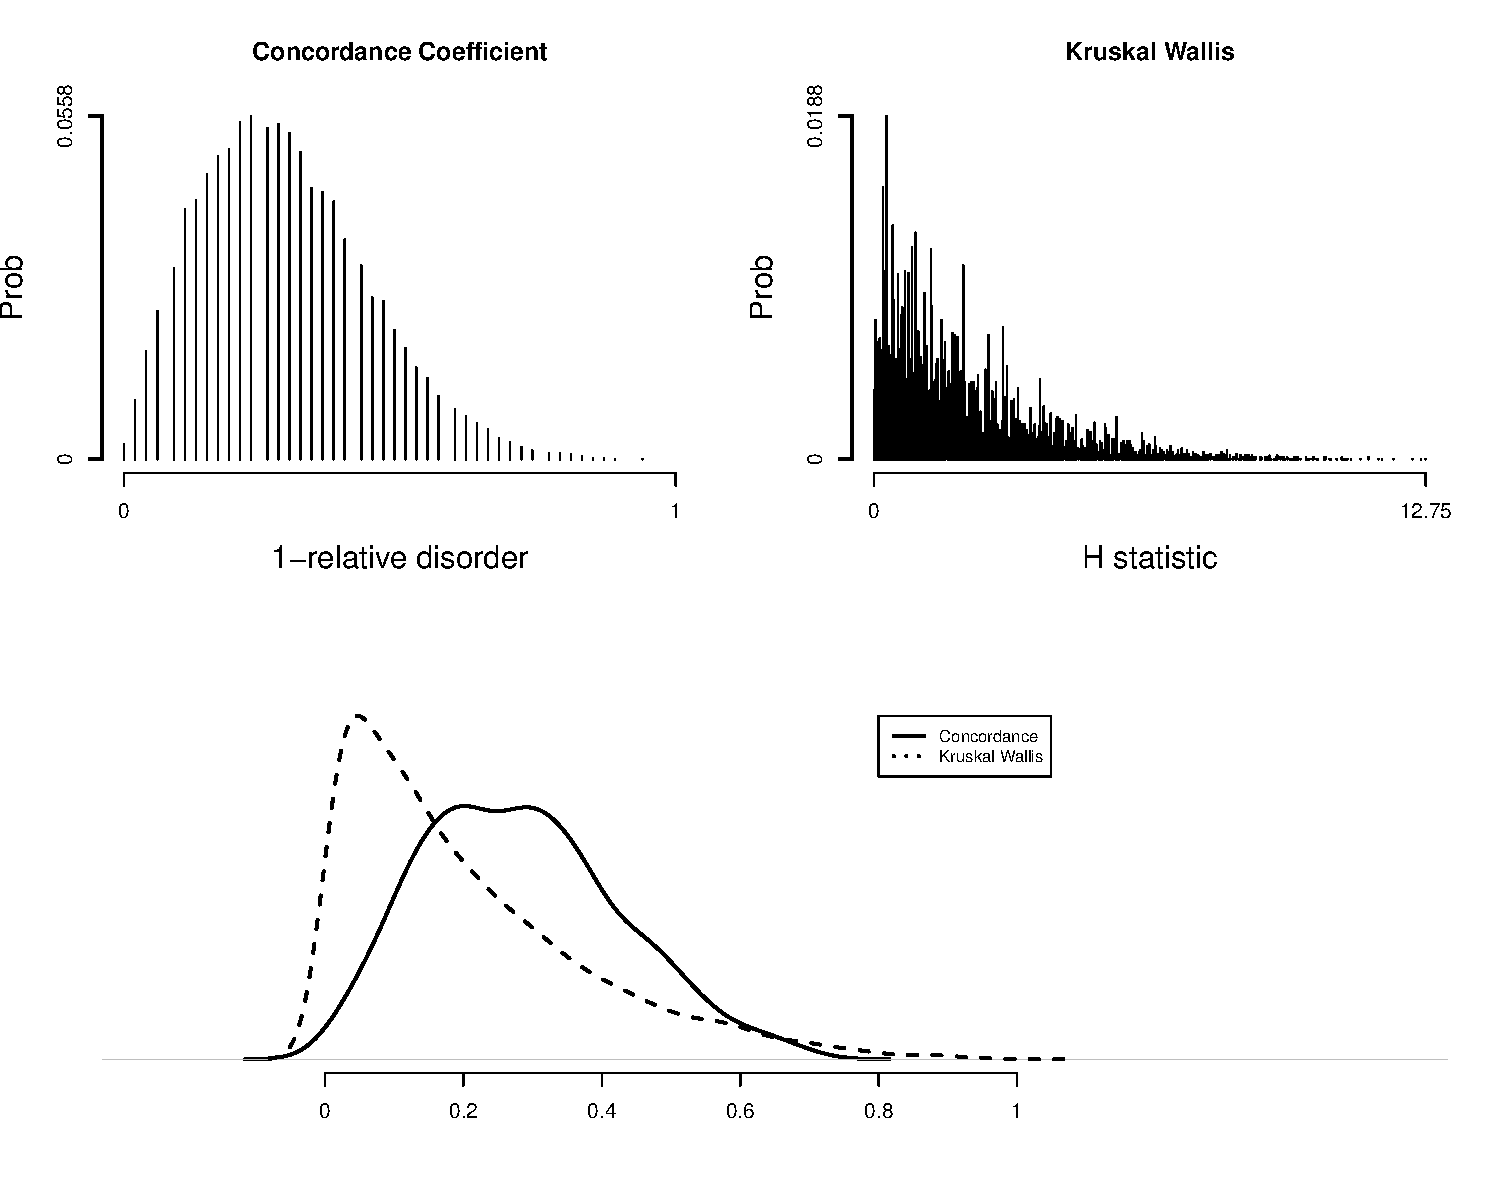
\includegraphics[width=11.5cm]{ProbabilityAndDensityDistributions}
\caption{\label{fig:1053} Probability distributions (first row) and density distributions (second row) of the Concordance coefficient ($\tau_c$=1-relative disorder) and the Kruskal-Wallis statistic ($H$), with sample sizes $N=(10,5,3)$.}
\end{figure}

As we mentioned in Figure~\ref{fig:distprob_222}, Figure~\ref{fig:1053} also shows that similar values of the Kruskal-Wallis statistic present very different probabilities, and this leads to a less smooth function than that presented by the Concordance coefficient. We can also see that the Concordance coefficient presents a more symmetrical distribution. This performance is generalized and, therefore, we consider that the Concordance coefficient is more reliable than the Kruskal-Wallis statistic.

The \pkg{ConcordanceTest} package also contains the function \code{LOP()}, which solves the Linear Ordering Problem from a square data matrix. This function allows to calculate the disorder of a permutation of elements from the preference matrix induced by that permutation and, therefore, it is necessary for the calculation of the Concordance coefficient. The function \code{LOP()} is used by functions \code{CT\_Distribution()}, \code{CT\_Hypothesis\_Test()} and \code{CT\_Coefficient()}. It is used as follows: 
\begin{example}
LOP(mat_LOP)
\end{example}
where \code{mat\_LOP} is the preference matrix defining the Linear Ordering Problem, a numeric square matrix for which we want to obtain the permutation of rows/columns that maximizes the sum of the elements above the main diagonal.

The function \code{LOP()} returns a list with the following elements: \code{obj\_val} is the optimal value of the solution of the Linear Ordering Problem, that is, the sum of the elements above the main diagonal under the permutation rows/columns solution, \code{permutation} is the solution of the Linear Ordering Problem, that is, the rows/columns permutation, and \code{permutation\_matrix} is the optimal permutation matrix of the Linear Ordering Problem.

\setcounter{exmp}{1}
\begin{exmp}[Cont.]
The matrix of preferences between treatments observed in Example~\ref{ex:18patients} was:

\begin{center}	\begin{tabular}{cccc}
		&\,\,\, \,\, $A$ & $B$ & $C$\,\,\,\, \\ 
		$A$&\multirow{3}{*}{  $ \left(\begin{array}{r}  $--$ \\7 \\  11 \end{array}\right.$}  &\multirow{3}{*}{  $ \begin{array}{c}43   \\ $--$  \\  13\end{array}$}   &\multirow{3}{*}{  $ \left.\begin{array}{c}19   \\2  \\  $--$ \end{array}\right)$}  \\
		$B$&&&\\
		$C$&&&\\
	\end{tabular}\end{center}
	
If we apply the function \code{LOP()} on this preference matrix we obtain the following results: 
\end{exmp}
%
\begin{example}
mat_LOP <- matrix(c(0,7,11,43,0,13,19,2,0), nrow=3)
LOP(mat_LOP)

$obj_val
[1] 75

$permutation
[1] 1 3 2

$permutation_matrix
     [,1] [,2] [,3]
[1,]    0    1    1
[2,]    0    0    0
[3,]    0    1    0
\end{example}

As we saw previously, the order between treatments that maximizes the order between patients corresponds to the order $(A\ C\ B)$ (\code{permutation} = 1 3 2), satisfying \code{obj\_val} = 75 of the preferences contained in the matrix.

 
\section{Comparison with \code{kruskal.test()} function from \pkg{stats} package}\label{sec:kruskal.test}

The well-known \pkg{stats} package contains, among many other functions, the function \code{kruskal.test()} that performs a Kruskal-Wallis rank sum test. In this section, we compare the results obtained with the \pkg{ConcordanceTest} package presented in this work and the function \code{kruskal.test()}, making use of the dataset from \cite{Hollander1973} referenced in the \code{kruskal.test()} examples.

\setcounter{exmp}{3}
\begin{exmp} \label{ex:4}
Comparison of \code{kruskal.test()} (\pkg{stats} package) and \code{CT\_Hypothesis\_Test()} functions with 25,000 simulations (\pkg{ConcordanceTest} package) using the dataset from \cite{Hollander1973}.
\begin{example}
## Hollander & Wolfe (1973), 116.
## Mucociliary efficiency from the rate of removal of dust in normal
##  subjects, subjects with obstructive airway disease, and subjects
##  with asbestosis.

x <- c(2.9, 3.0, 2.5, 2.6, 3.2) # normal subjects
y <- c(3.8, 2.7, 4.0, 2.4)      # with obstructive airway disease
z <- c(2.8, 3.4, 3.7, 2.2, 2.0) # with asbestosis
Sample_List <- list(x, y, z)

kruskal.test(Sample_List)

	Kruskal-Wallis rank sum test

data:  Sample_List
Kruskal-Wallis chi-squared = 0.77143, df = 2, p-value = 0.68

set.seed(12)
CT_Hypothesis_Test(Sample_List, Num_Sim = 25000, H = 1)

results
                        Statistic p-value
Concordance coefficient     0.188 0.78408
Kruskal-Wallis              0.771 0.71080

$C_p_value
[1] 0.78408

$H_p_value
[1] 0.7108

\end{example}

\end{exmp}

As can be observed, the value of the Kruskal-Wallis statistic is the same with both functions (0.771). However, the p-values associated with the statistic differ. 

The Kruskal-Wallis statistic follows approximately a $\chi^2$ distribution with degrees of freedom equal to the number of groups minus 1 \citep{Kruskal1952}. For this reason, the function \code{kruskal.test()} uses a $\chi^2$ distribution to approximate the p-value (using the function \code{pchisq()}). In the case of the function \code{CT\_Hypothesis\_Test()}, it calculates the p-values using the simulations performed (25,000 in this example).

The function \code{CT\_Distribution()} of the \pkg{ConcordanceTest} package allows the probability distribution tables of the Concordance coefficient and Kruskal-Wallis statistic to be computed, and they can be obtained exactly or by simulation. We can get the exact probability distribution tables and, consequently, the exact p-values in Example~\ref{ex:4} with
\begin{example}
CT_Distribution(c(5,4,5), Num_Sim = 0, H = 1)
\end{example}

In Example~\ref{ex:4}, the exact p-value for the Kruskal-Wallis statistic is 0.71077. Therefore, the difference between our p-value obtained with 25,000 simulations (0.71080) and the exact one is 0.00003, while the difference between the p-value approximated by the $\chi^2$ distribution (0.68) and the exact one is 0.03077. Regarding the Concordance coefficient, the exact p-value is 0.78468, hence, the difference between our p-value obtained with 25,000 simulations (0.78408) and the exact one is 0.0006.

It is worth noting that the function \code{kruskal.test()} uses the $\chi^2$ distribution to approximate the p-value regardless of the size of the samples, but \cite{Kruskal1952} state that the Kruskal-Wallis statistic is distributed approximately as a $\chi^2$, unless the samples are too small, in which case special approximations or exact tables should be provided. On the contrary, the \pkg{ConcordanceTest} package can always obtain a good approximation of the p-values, regardless of the size of the samples, as long as a high number of simulations is used.


\section{Final remarks and future research} \label{sec:conclusion}

A new measure based on the Kendall-$\tau$ distance is presented in this work to estimate the \emph{concordance} of different samples. A statistical test to determine when different observations come from the same distribution is also introduced. A comparison with the classical Kruskal-Wallis test is introduced to show that both tests differ. As we have shown, the proposed coefficient is more appropriate and reliable than rank-based methods. This work also describes the R package \pkg{ConcordanceTest} \citep{ConcordanceTest2022}, which contains all the functions needed to work with the proposed Concordance coefficient and allows its comparison with the Kruskal-Wallis statistic.

This work  aims to be an introduction of the new concordance measure between samples, but there still remains much to be done. There is a new problem and further challenges for researchers, for example: studying the asymptotic distribution of the Concordance coefficient, exploring the possibility of finding the exact distribution with the help of modern computing, or analyzing the power of the Concordance test presented in this work, among others.

\section{Acknowledgments}

The authors thank the grants PID2019-105952GB-I00 funded by Ministerio de Ciencia e Innovación/ Agencia Estatal de Investigación /10.13039/501100011033, Spain, and PROMETEO/2021/063 funded by the government of the Valencian Community, Spain.

\bibliography{ConcordanceTestRJ}



\newpage

\begin{appendix}

\section{Appendix A: Results in the experiment with sample sizes $N=(2,2,2)$} \label{A:222}

Table~\ref{samplespace222} shows the Concordance coefficient ($\tau_c$) and Kruskal-Wallis statistic ($H$) for all possible results in an experiment with three treatments and two people in each treatment.

\setlength{\tabcolsep}{.5mm} 
\renewcommand{\arraystretch}{.001}
\renewcommand{\arraystretch}{.85}

\begin{table}[h] 	\centering \footnotesize
\begin{tabular}{cccccccccccccccccccccccccccccccccccccccccc}  
 &&&&&&&& $dis$ &&  $\tau_c$ &$H$&&&&&&&&&&&& $dis$ &&  $\tau_c$ & $H$&&&&&&&&&&&&  $dis$ &&  $\tau_c$ &$H$\\
\toprule
	&	a	&	a	&	b	&	b	&	c	&	c	&&	0	&&	1.0000	&	4.57	&&	&&	&	b	&	a	&	a	&	b	&	c	&	c	&&	2	&&	0.6667	&	3.43	&&	&&	&	c	&	a	&	a	&	b	&	b	&	c	&&	4	&&	0.3333	&	1.14	\\	\cmidrule(l){1-12}		\cmidrule(l){16-27}		\cmidrule(l){31-42}
	&	a	&	a	&	b	&	c	&	b	&	c	&&	1	&&	0.8333	&	3.71	&&	&&	&	b	&	a	&	a	&	c	&	b	&	c	&&	3	&&	0.5000	&	2.00	&&	&&	&	c	&	a	&	a	&	b	&	c	&	b	&&	3	&&	0.5000	&	2.00	\\	\cmidrule(l){1-12}		\cmidrule(l){16-27}		\cmidrule(l){31-42}
	&	a	&	a	&	b	&	c	&	c	&	b	&&	2	&&	0.6667	&	3.43	&&	&&	&	b	&	a	&	a	&	c	&	c	&	b	&&	4	&&	0.3333	&	1.14	&&	&&	&	c	&	a	&	a	&	c	&	b	&	b	&&	2	&&	0.6667	&	3.43	\\	\cmidrule(l){1-12}		\cmidrule(l){16-27}		\cmidrule(l){31-42}
	&	a	&	a	&	c	&	b	&	b	&	c	&&	2	&&	0.6667	&	3.43	&&	&&	&	b	&	a	&	b	&	a	&	c	&	c	&&	1	&&	0.8333	&	3.71	&&	&&	&	c	&	a	&	b	&	a	&	b	&	c	&&	5	&&	0.1667	&	0.29	\\	\cmidrule(l){1-12}		\cmidrule(l){16-27}		\cmidrule(l){31-42}
	&	a	&	a	&	c	&	b	&	c	&	b	&&	1	&&	0.8333	&	3.71	&&	&&	&	b	&	a	&	b	&	c	&	a	&	c	&&	2	&&	0.6667	&	2.57	&&	&&	&	c	&	a	&	b	&	a	&	c	&	b	&&	4	&&	0.3333	&	0.86	\\	\cmidrule(l){1-12}		\cmidrule(l){16-27}		\cmidrule(l){31-42}
	&	a	&	a	&	c	&	c	&	b	&	b	&&	0	&&	1.0000	&	4.57	&&	&&	&	b	&	a	&	b	&	c	&	c	&	a	&&	3	&&	0.5000	&	2.00	&&	&&	&	c	&	a	&	b	&	b	&	a	&	c	&&	6	&&	0.0000	&	0.00	\\	\cmidrule(l){1-12}		\cmidrule(l){16-27}		\cmidrule(l){31-42}
	&	a	&	b	&	a	&	b	&	c	&	c	&&	1	&&	0.8333	&	3.71	&&	&&	&	b	&	a	&	c	&	a	&	b	&	c	&&	4	&&	0.3333	&	0.86	&&	&&	&	c	&	a	&	b	&	b	&	c	&	a	&&	5	&&	0.1667	&	0.29	\\	\cmidrule(l){1-12}		\cmidrule(l){16-27}		\cmidrule(l){31-42}
	&	a	&	b	&	a	&	c	&	b	&	c	&&	2	&&	0.6667	&	2.57	&&	&&	&	b	&	a	&	c	&	a	&	c	&	b	&&	5	&&	0.1667	&	0.29	&&	&&	&	c	&	a	&	b	&	c	&	a	&	b	&&	3	&&	0.5000	&	1.14	\\	\cmidrule(l){1-12}		\cmidrule(l){16-27}		\cmidrule(l){31-42}
	&	a	&	b	&	a	&	c	&	c	&	b	&&	3	&&	0.5000	&	2.00	&&	&&	&	b	&	a	&	c	&	b	&	a	&	c	&&	3	&&	0.5000	&	1.14	&&	&&	&	c	&	a	&	b	&	c	&	b	&	a	&&	4	&&	0.3333	&	0.86	\\	\cmidrule(l){1-12}		\cmidrule(l){16-27}		\cmidrule(l){31-42}
	&	a	&	b	&	b	&	a	&	c	&	c	&&	2	&&	0.6667	&	3.43	&&	&&	&	b	&	a	&	c	&	b	&	c	&	a	&&	4	&&	0.3333	&	0.86	&&	&&	&	c	&	a	&	c	&	a	&	b	&	b	&&	1	&&	0.8333	&	3.71	\\	\cmidrule(l){1-12}		\cmidrule(l){16-27}		\cmidrule(l){31-42}
	&	a	&	b	&	b	&	c	&	a	&	c	&&	3	&&	0.5000	&	2.00	&&	&&	&	b	&	a	&	c	&	c	&	a	&	b	&&	6	&&	0.0000	&	0.00	&&	&&	&	c	&	a	&	c	&	b	&	a	&	b	&&	2	&&	0.6667	&	2.57	\\	\cmidrule(l){1-12}		\cmidrule(l){16-27}		\cmidrule(l){31-42}
	&	a	&	b	&	b	&	c	&	c	&	a	&&	4	&&	0.3333	&	1.14	&&	&&	&	b	&	a	&	c	&	c	&	b	&	a	&&	5	&&	0.1667	&	0.29	&&	&&	&	c	&	a	&	c	&	b	&	b	&	a	&&	3	&&	0.5000	&	2.00	\\	\cmidrule(l){1-12}		\cmidrule(l){16-27}		\cmidrule(l){31-42}
	&	a	&	b	&	c	&	a	&	b	&	c	&&	3	&&	0.5000	&	1.14	&&	&&	&	b	&	b	&	a	&	a	&	c	&	c	&&	0	&&	1.0000	&	4.57	&&	&&	&	c	&	b	&	a	&	a	&	b	&	c	&&	6	&&	0.0000	&	0.00	\\	\cmidrule(l){1-12}		\cmidrule(l){16-27}		\cmidrule(l){31-42}
	&	a	&	b	&	c	&	a	&	c	&	b	&&	4	&&	0.3333	&	0.86	&&	&&	&	b	&	b	&	a	&	c	&	a	&	c	&&	1	&&	0.8333	&	3.71	&&	&&	&	c	&	b	&	a	&	a	&	c	&	b	&&	5	&&	0.1667	&	0.29	\\	\cmidrule(l){1-12}		\cmidrule(l){16-27}		\cmidrule(l){31-42}
	&	a	&	b	&	c	&	b	&	a	&	c	&&	4	&&	0.3333	&	0.86	&&	&&	&	b	&	b	&	a	&	c	&	c	&	a	&&	2	&&	0.6667	&	3.43	&&	&&	&	c	&	b	&	a	&	b	&	a	&	c	&&	5	&&	0.1667	&	0.29	\\	\cmidrule(l){1-12}		\cmidrule(l){16-27}		\cmidrule(l){31-42}
	&	a	&	b	&	c	&	b	&	c	&	a	&&	5	&&	0.1667	&	0.29	&&	&&	&	b	&	b	&	c	&	a	&	a	&	c	&&	2	&&	0.6667	&	3.43	&&	&&	&	c	&	b	&	a	&	b	&	c	&	a	&&	4	&&	0.3333	&	0.86	\\	\cmidrule(l){1-12}		\cmidrule(l){16-27}		\cmidrule(l){31-42}
	&	a	&	b	&	c	&	c	&	a	&	b	&&	5	&&	0.1667	&	0.29	&&	&&	&	b	&	b	&	c	&	a	&	c	&	a	&&	1	&&	0.8333	&	3.71	&&	&&	&	c	&	b	&	a	&	c	&	a	&	b	&&	4	&&	0.3333	&	0.86	\\	\cmidrule(l){1-12}		\cmidrule(l){16-27}		\cmidrule(l){31-42}
	&	a	&	b	&	c	&	c	&	b	&	a	&&	6	&&	0.0000	&	0.00	&&	&&	&	b	&	b	&	c	&	c	&	a	&	a	&&	0	&&	1.0000	&	4.57	&&	&&	&	c	&	b	&	a	&	c	&	b	&	a	&&	3	&&	0.5000	&	1.14	\\	\cmidrule(l){1-12}		\cmidrule(l){16-27}		\cmidrule(l){31-42}
	&	a	&	c	&	a	&	b	&	b	&	c	&&	3	&&	0.5000	&	2.00	&&	&&	&	b	&	c	&	a	&	a	&	b	&	c	&&	5	&&	0.1667	&	0.29	&&	&&	&	c	&	b	&	b	&	a	&	a	&	c	&&	4	&&	0.3333	&	1.14	\\	\cmidrule(l){1-12}		\cmidrule(l){16-27}		\cmidrule(l){31-42}
	&	a	&	c	&	a	&	b	&	c	&	b	&&	2	&&	0.6667	&	2.57	&&	&&	&	b	&	c	&	a	&	a	&	c	&	b	&&	6	&&	0.0000	&	0.00	&&	&&	&	c	&	b	&	b	&	a	&	c	&	a	&&	3	&&	0.5000	&	2.00	\\	\cmidrule(l){1-12}		\cmidrule(l){16-27}		\cmidrule(l){31-42}
	&	a	&	c	&	a	&	c	&	b	&	b	&&	1	&&	0.8333	&	3.71	&&	&&	&	b	&	c	&	a	&	b	&	a	&	c	&&	4	&&	0.3333	&	0.86	&&	&&	&	c	&	b	&	b	&	c	&	a	&	a	&&	2	&&	0.6667	&	3.43	\\	\cmidrule(l){1-12}		\cmidrule(l){16-27}		\cmidrule(l){31-42}
	&	a	&	c	&	b	&	a	&	b	&	c	&&	4	&&	0.3333	&	0.86	&&	&&	&	b	&	c	&	a	&	b	&	c	&	a	&&	3	&&	0.5000	&	1.14	&&	&&	&	c	&	b	&	c	&	a	&	a	&	b	&&	3	&&	0.5000	&	2.00	\\	\cmidrule(l){1-12}		\cmidrule(l){16-27}		\cmidrule(l){31-42}
	&	a	&	c	&	b	&	a	&	c	&	b	&&	3	&&	0.5000	&	1.14	&&	&&	&	b	&	c	&	a	&	c	&	a	&	b	&&	5	&&	0.1667	&	0.29	&&	&&	&	c	&	b	&	c	&	a	&	b	&	a	&&	2	&&	0.6667	&	2.57	\\	\cmidrule(l){1-12}		\cmidrule(l){16-27}		\cmidrule(l){31-42}
	&	a	&	c	&	b	&	b	&	a	&	c	&&	5	&&	0.1667	&	0.29	&&	&&	&	b	&	c	&	a	&	c	&	b	&	a	&&	4	&&	0.3333	&	0.86	&&	&&	&	c	&	b	&	c	&	b	&	a	&	a	&&	1	&&	0.8333	&	3.71	\\	\cmidrule(l){1-12}		\cmidrule(l){16-27}		\cmidrule(l){31-42}
	&	a	&	c	&	b	&	b	&	c	&	a	&&	6	&&	0.0000	&	0.00	&&	&&	&	b	&	c	&	b	&	a	&	a	&	c	&&	3	&&	0.5000	&	2.00	&&	&&	&	c	&	c	&	a	&	a	&	b	&	b	&&	0	&&	1.0000	&	4.57	\\	\cmidrule(l){1-12}		\cmidrule(l){16-27}		\cmidrule(l){31-42}
	&	a	&	c	&	b	&	c	&	a	&	b	&&	4	&&	0.3333	&	0.86	&&	&&	&	b	&	c	&	b	&	a	&	c	&	a	&&	2	&&	0.6667	&	2.57	&&	&&	&	c	&	c	&	a	&	b	&	a	&	b	&&	1	&&	0.8333	&	3.71	\\	\cmidrule(l){1-12}		\cmidrule(l){16-27}		\cmidrule(l){31-42}
	&	a	&	c	&	b	&	c	&	b	&	a	&&	5	&&	0.1667	&	0.29	&&	&&	&	b	&	c	&	b	&	c	&	a	&	a	&&	1	&&	0.8333	&	3.71	&&	&&	&	c	&	c	&	a	&	b	&	b	&	a	&&	2	&&	0.6667	&	3.43	\\	\cmidrule(l){1-12}		\cmidrule(l){16-27}		\cmidrule(l){31-42}
	&	a	&	c	&	c	&	a	&	b	&	b	&&	2	&&	0.6667	&	3.43	&&	&&	&	b	&	c	&	c	&	a	&	a	&	b	&&	4	&&	0.3333	&	1.14	&&	&&	&	c	&	c	&	b	&	a	&	a	&	b	&&	2	&&	0.6667	&	3.43	\\	\cmidrule(l){1-12}		\cmidrule(l){16-27}		\cmidrule(l){31-42}
	&	a	&	c	&	c	&	b	&	a	&	b	&&	3	&&	0.5000	&	2.00	&&	&&	&	b	&	c	&	c	&	a	&	b	&	a	&&	3	&&	0.5000	&	2.00	&&	&&	&	c	&	c	&	b	&	a	&	b	&	a	&&	1	&&	0.8333	&	3.71	\\	\cmidrule(l){1-12}		\cmidrule(l){16-27}		\cmidrule(l){31-42}
	&	a	&	c	&	c	&	b	&	b	&	a	&&	4	&&	0.3333	&	1.14	&&	&&	&	b	&	c	&	c	&	b	&	a	&	a	&&	2	&&	0.6667	&	3.43	&&	&&	&	c	&	c	&	b	&	b	&	a	&	a	&&	0	&&	1.0000	&	4.57	\\	\bottomrule[0.2mm]
\end{tabular}
	%\caption{All possible results in the experiment with sample sizes $N=(2,2,2)$ }
	\caption{Concordance coefficient ($\tau_c$) and Kruskal-Wallis statistic ($H$) for all possible results in an experiment with sample sizes $N=(2,2,2).$ }
       \label{samplespace222}
\end{table}

\newpage

\section{Appendix B: Comparison of distributions} \label{A:densityPlots}

Table~\ref{t:DensityPlots} shows the probability density function of the Concordance coefficient (continuous lines) and  the Kruskal-Wallis statistic (dashed lines) generated by simulation. Number of simulations 100,000. Note that the $H$ statistic has been normalized between 0 and 1. 

\renewcommand{\arraystretch}{.95}

%\scriptsize
\setlength{\tabcolsep}{1.65mm}
\begin{longtable}{ccc} \hline 
\endfirsthead

\multicolumn{3}{c}%
{{\bfseries \tablename\ \thetable{} -- continued from previous page}}  \\ \cline{1-3}
\endhead

\hline \multicolumn{3}{r}{{Continued on next page}} \\ \hline
\caption{Empirical density probability functions for several experiments (Concordance coefficient in continuous lines and Kruskal-Wallis statistic in dashed lines), where sample sizes vary form $N=(4,4)$ to $N=(5,5,4,4,4,4,4)$.} \label{t:DensityPlots}\\
\endfoot

%\hline 
\caption{Empirical density probability functions for several experiments (Concordance coefficient in continuous lines and Kruskal-Wallis statistic in dashed lines), where sample sizes vary form $N=(4,4)$ to $N=(5,5,4,4,4,4,4)$.}
\endlastfoot

\hline
		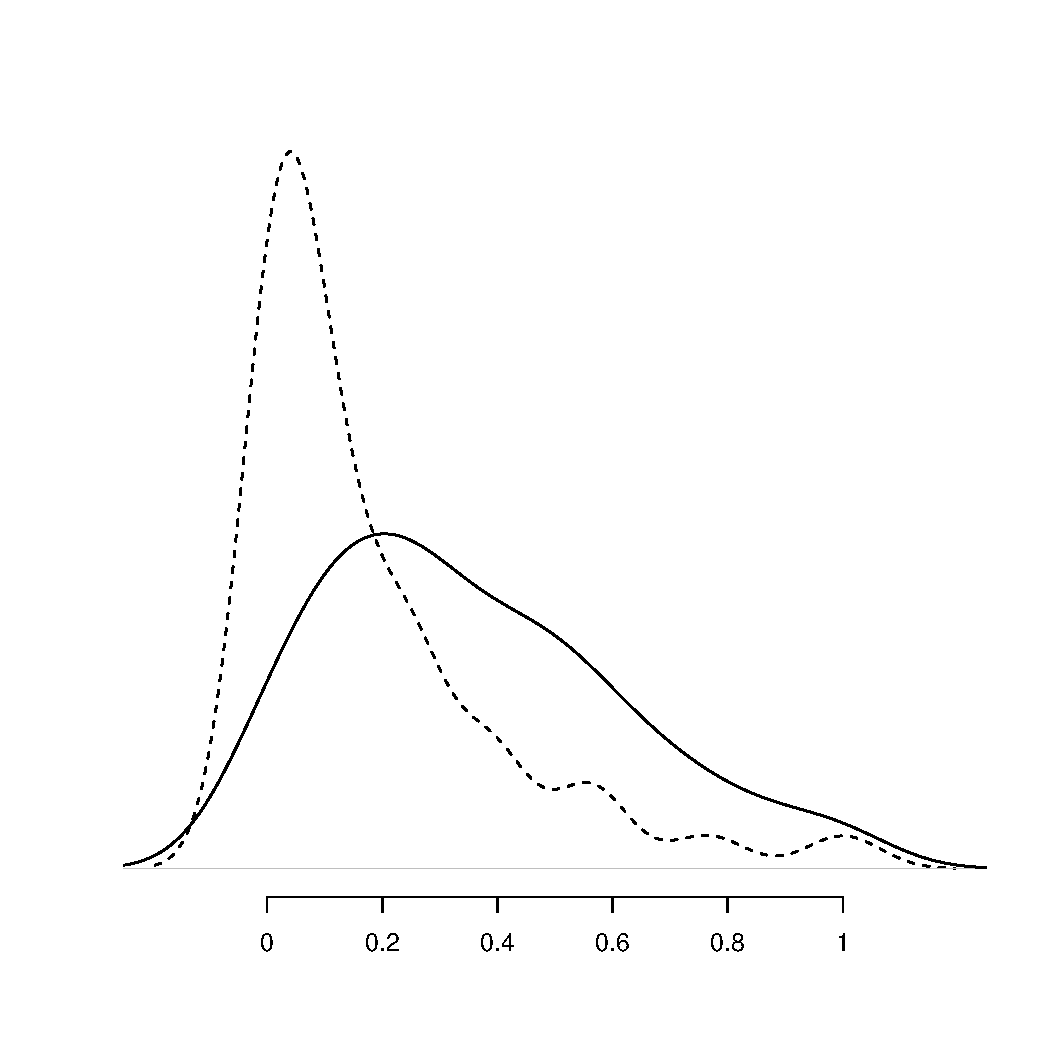
\includegraphics[width=4.05cm]{Sim_Kendall-Kruskal_44_b.pdf} & 
		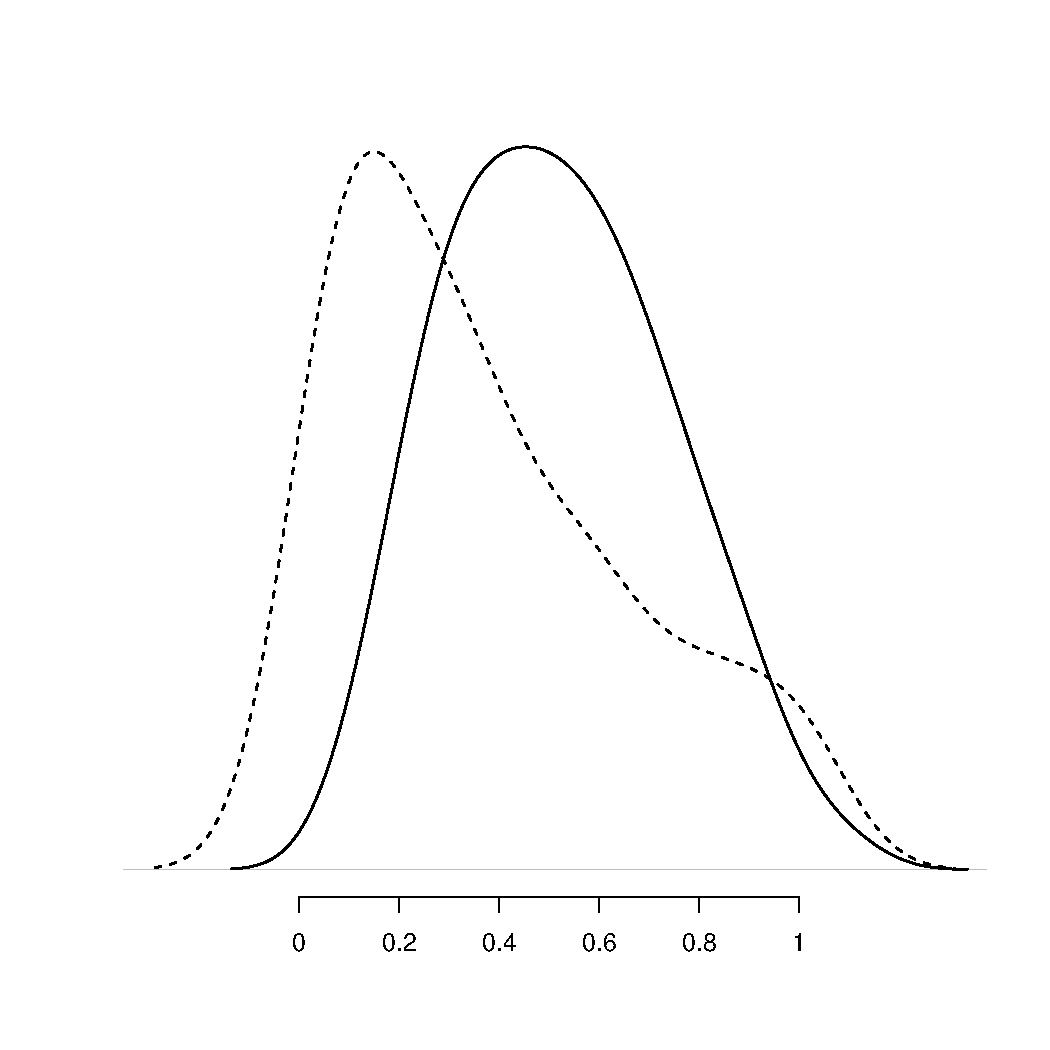
\includegraphics[width=4.05cm]{Sim_Kendall-Kruskal_332_b.pdf} & 
		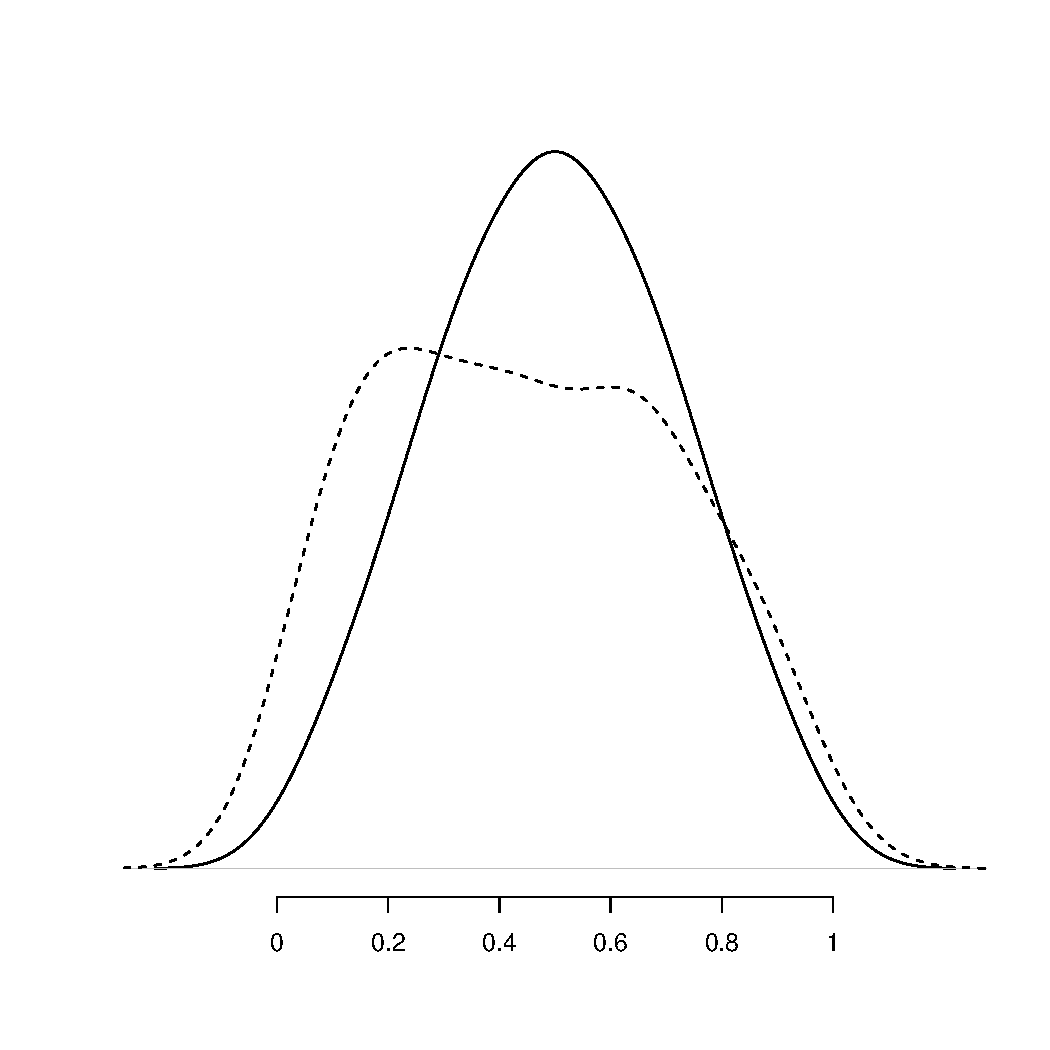
\includegraphics[width=4.05cm]{Sim_Kendall-Kruskal_2222_a.pdf} \\ 
		           Sample\_Sizes=(4,4)  &  Sample\_Sizes=(3,3,2)  &   Sample\_Sizes=(2,2,2,2) \\  
\hline 
	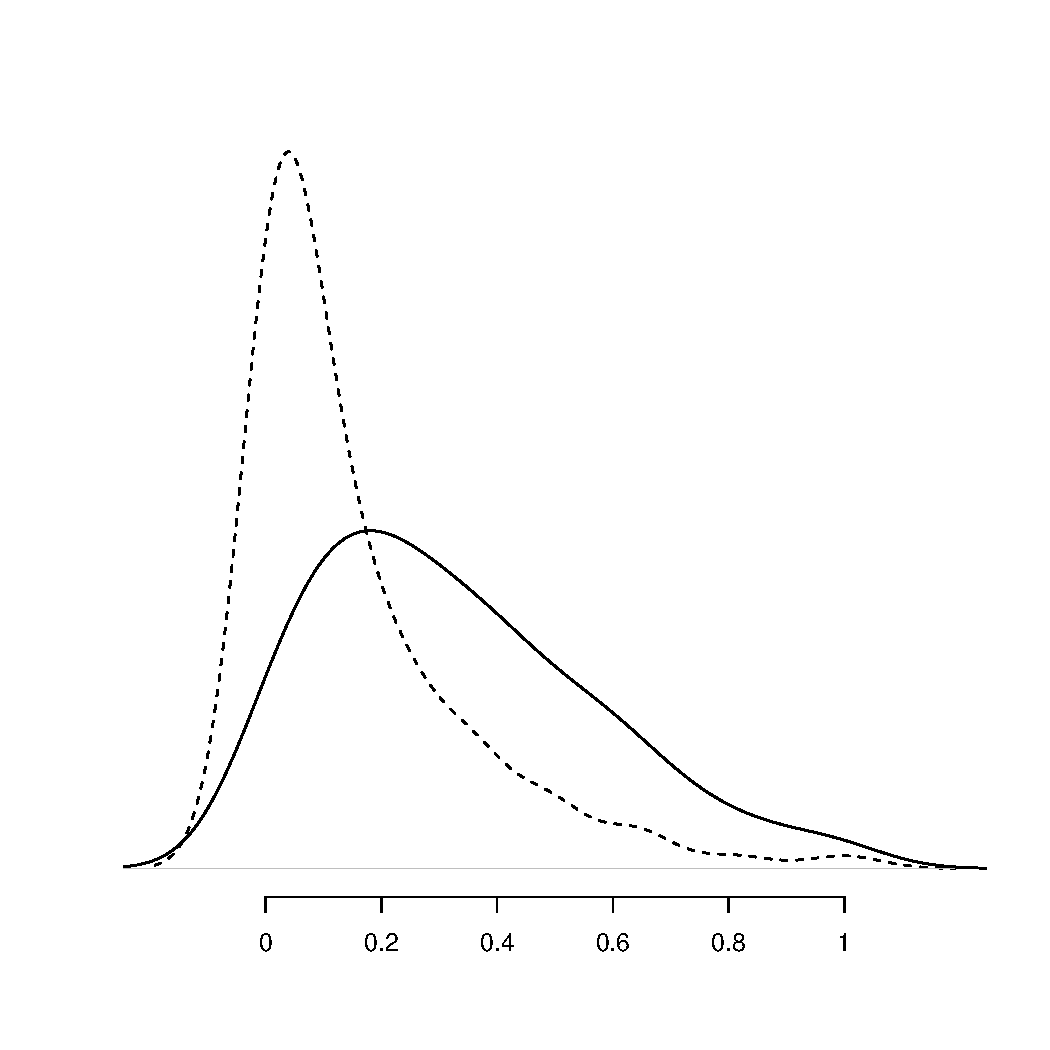
\includegraphics[width=4.05cm]{Sim_Kendall-Kruskal_54_b.pdf} & 
		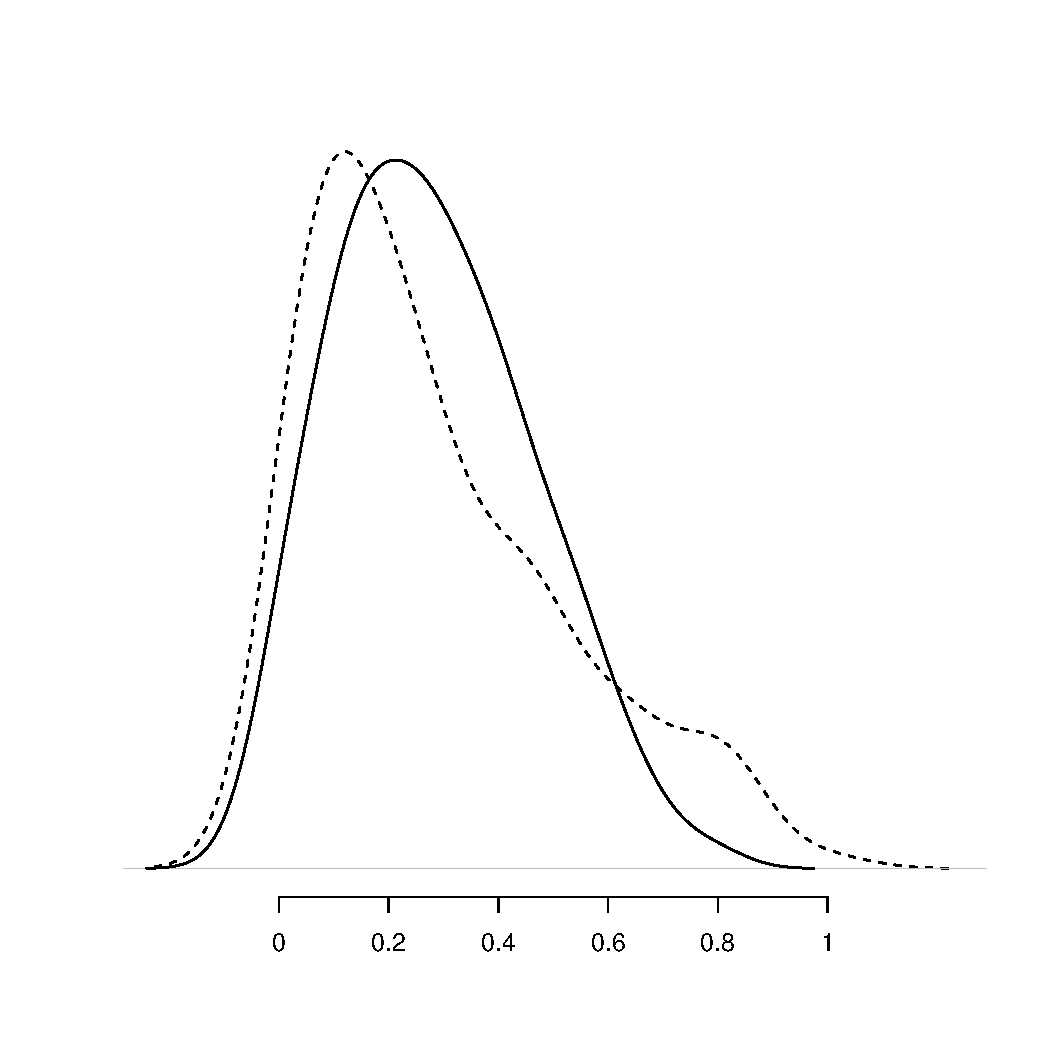
\includegraphics[width=4.05cm]{Sim_Kendall-Kruskal_333_b.pdf} & 
		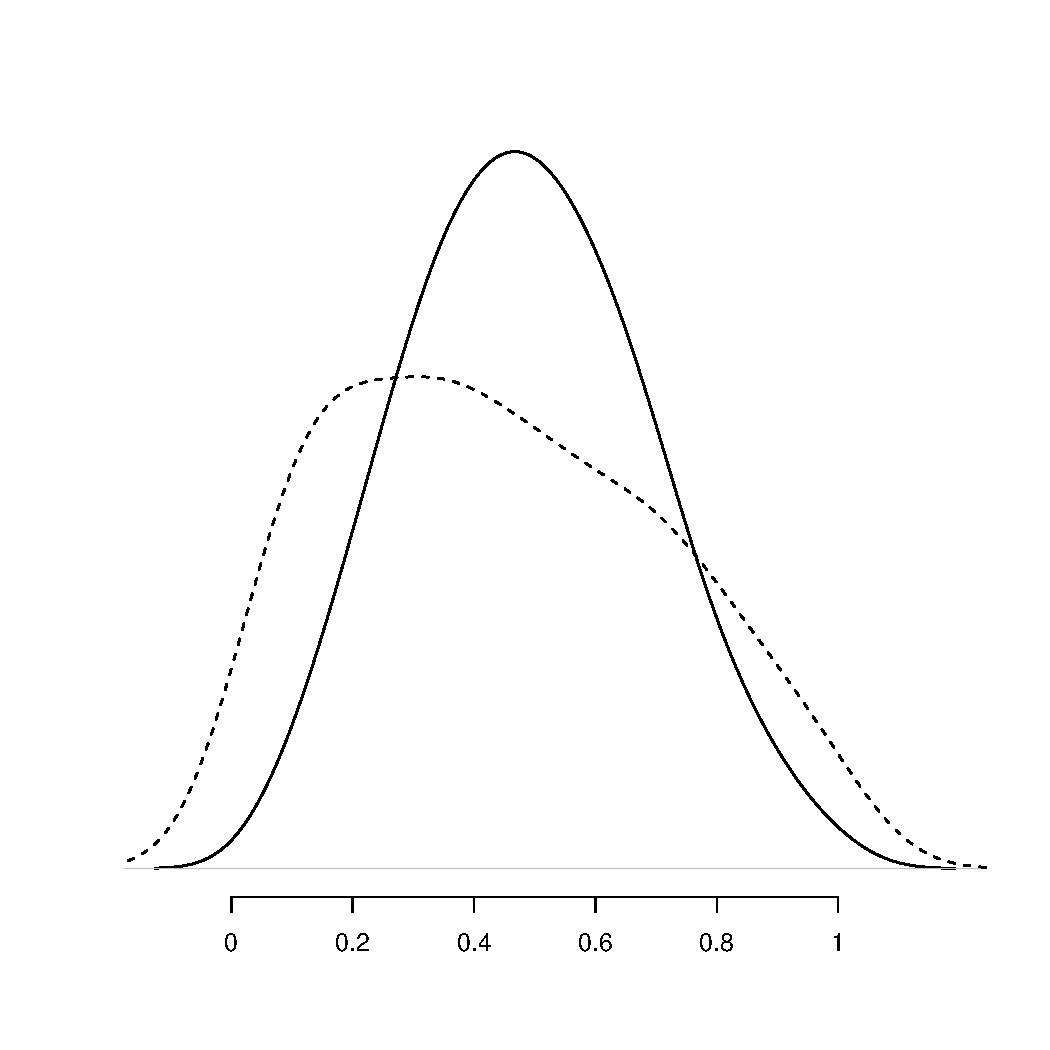
\includegraphics[width=4.05cm]{Sim_Kendall-Kruskal_3222_a.pdf} \\ 
		              Sample\_Sizes=(5,4) &   Sample\_Sizes=(3,3,3)  &    Sample\_Sizes=(3,2,2,2) \\  
\hline 
	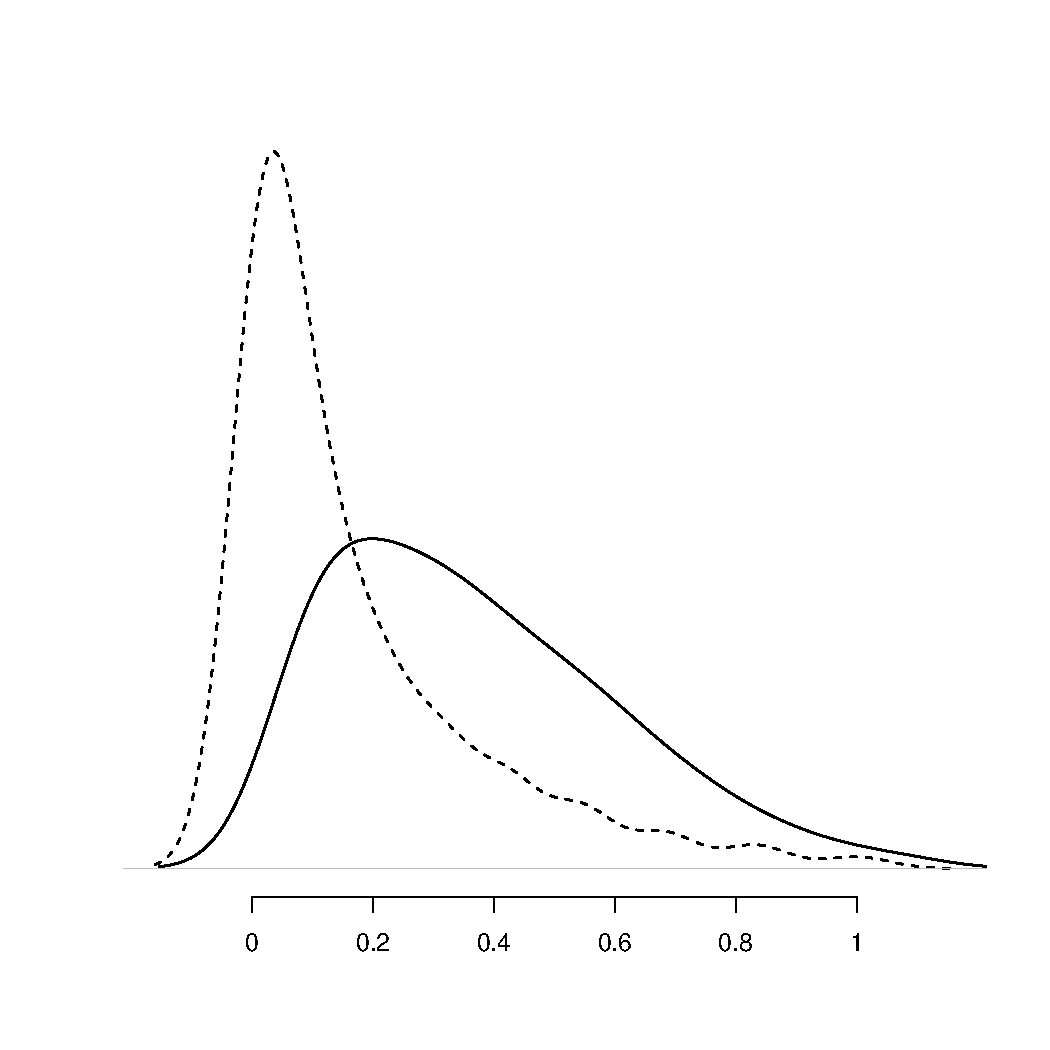
\includegraphics[width=4.05cm]{Sim_Kendall-Kruskal_55_b.pdf} & 
		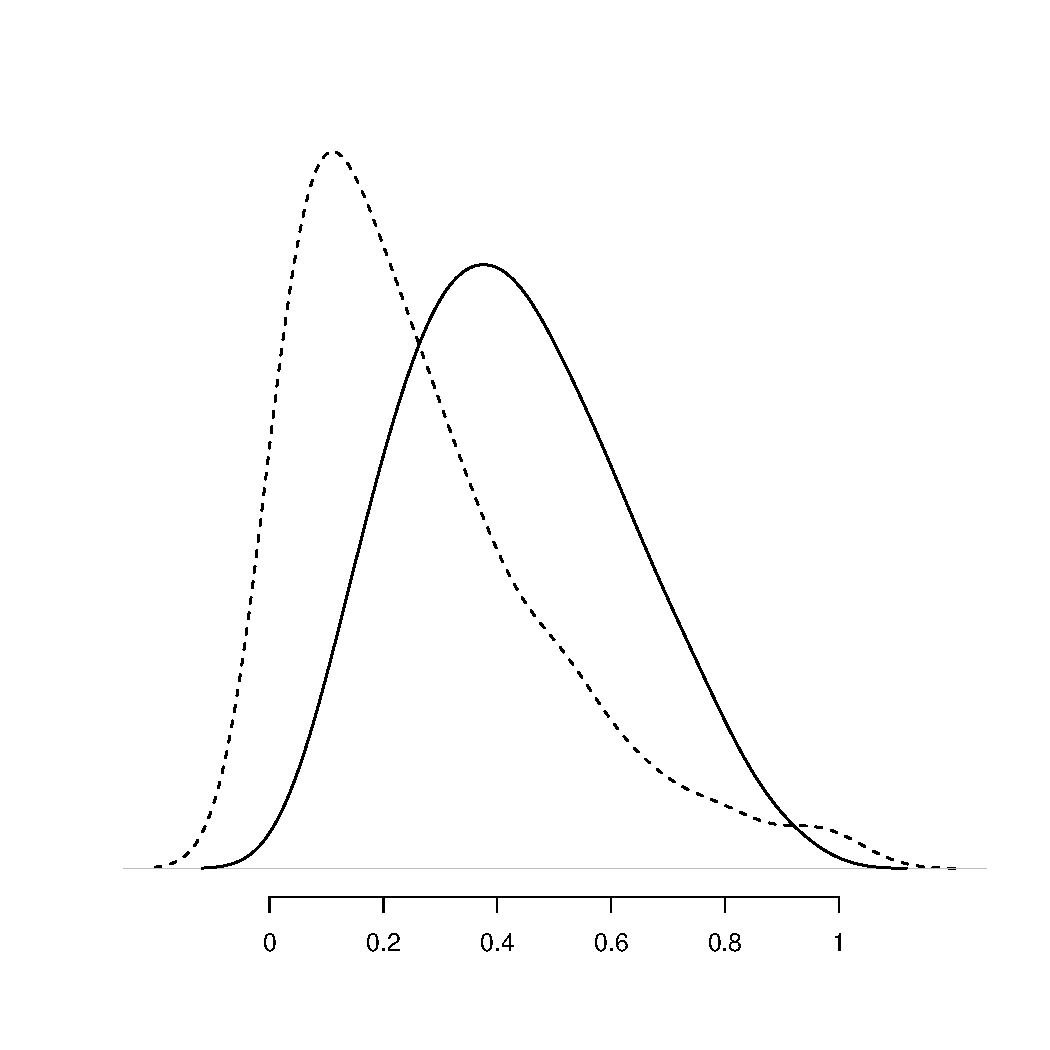
\includegraphics[width=4.05cm]{Sim_Kendall-Kruskal_433_b.pdf} & 
		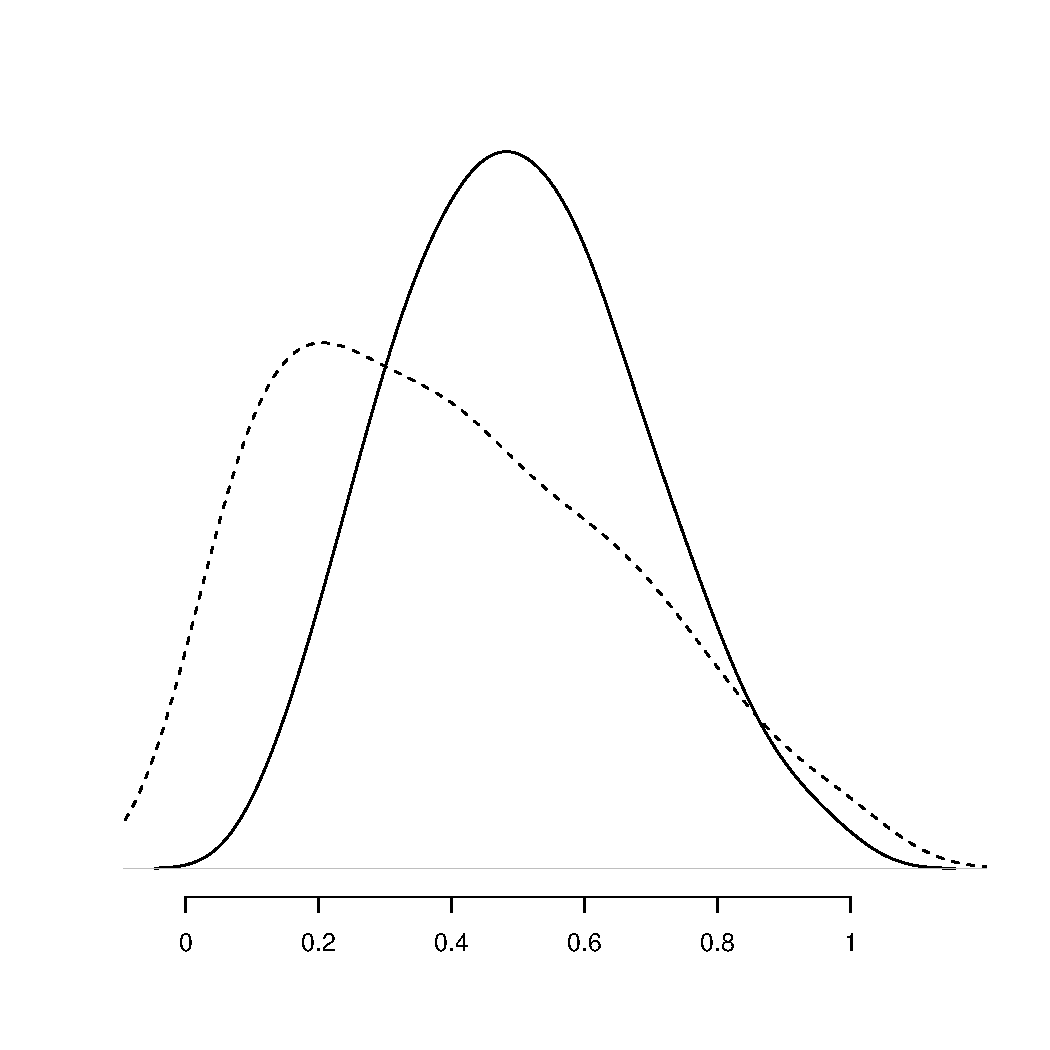
\includegraphics[width=4.05cm]{Sim_Kendall-Kruskal_3322_a.pdf} \\ 
		              Sample\_Sizes=(5,5) &   Sample\_Sizes=(4,3,3)  &    Sample\_Sizes=(3,3,2,2) \\  
		              \hline

		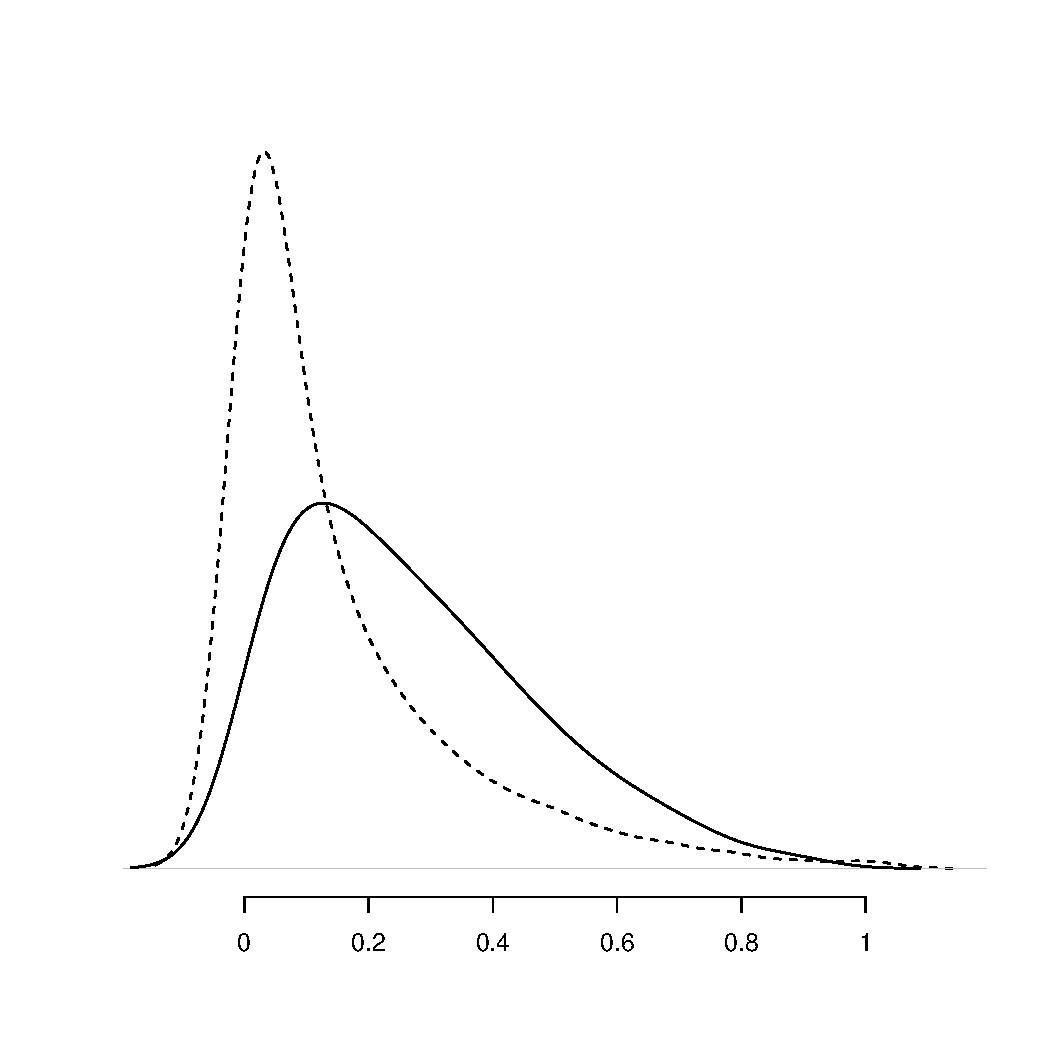
\includegraphics[width=4.05cm]{Sim_Kendall-Kruskal_76_b.pdf} & 
		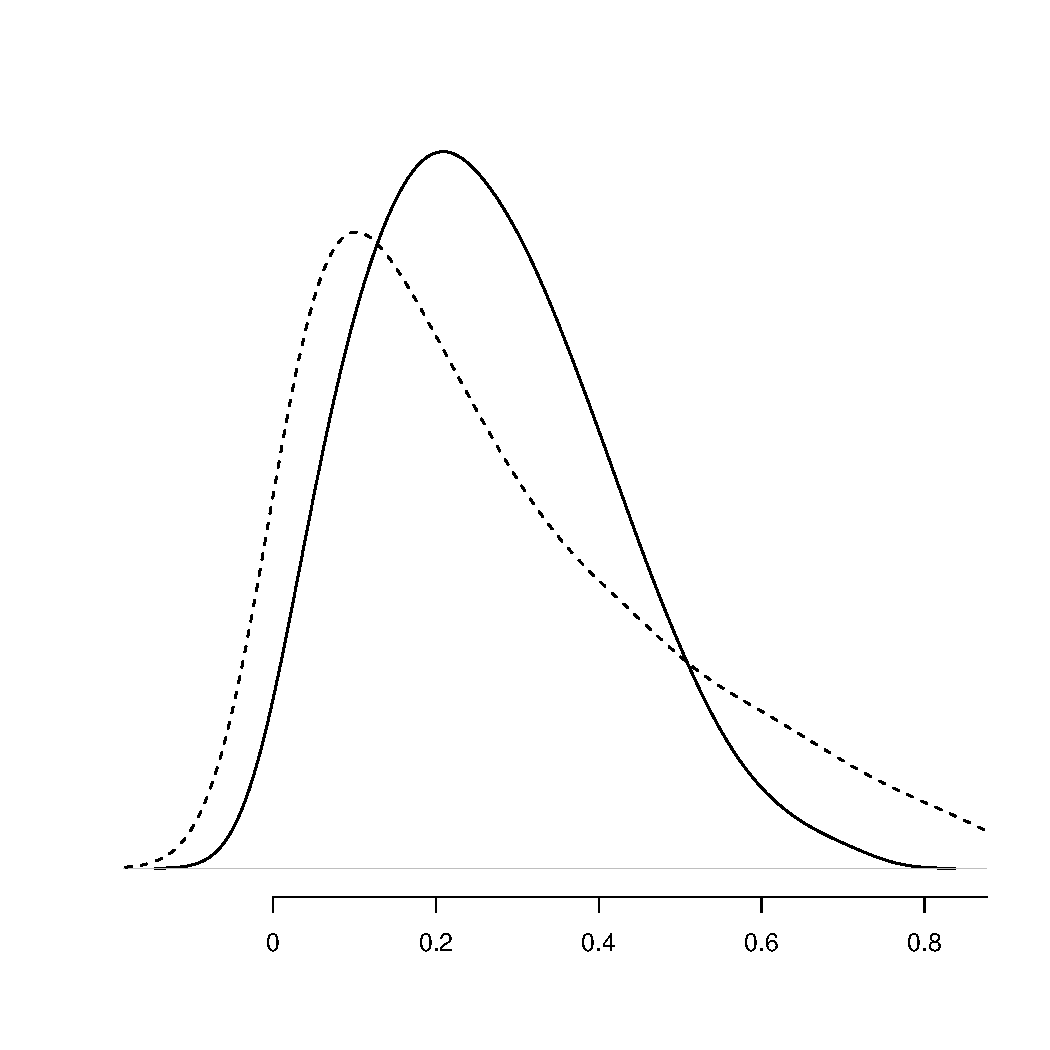
\includegraphics[width=4.05cm]{Sim_Kendall-Kruskal_555_a.pdf} & 
		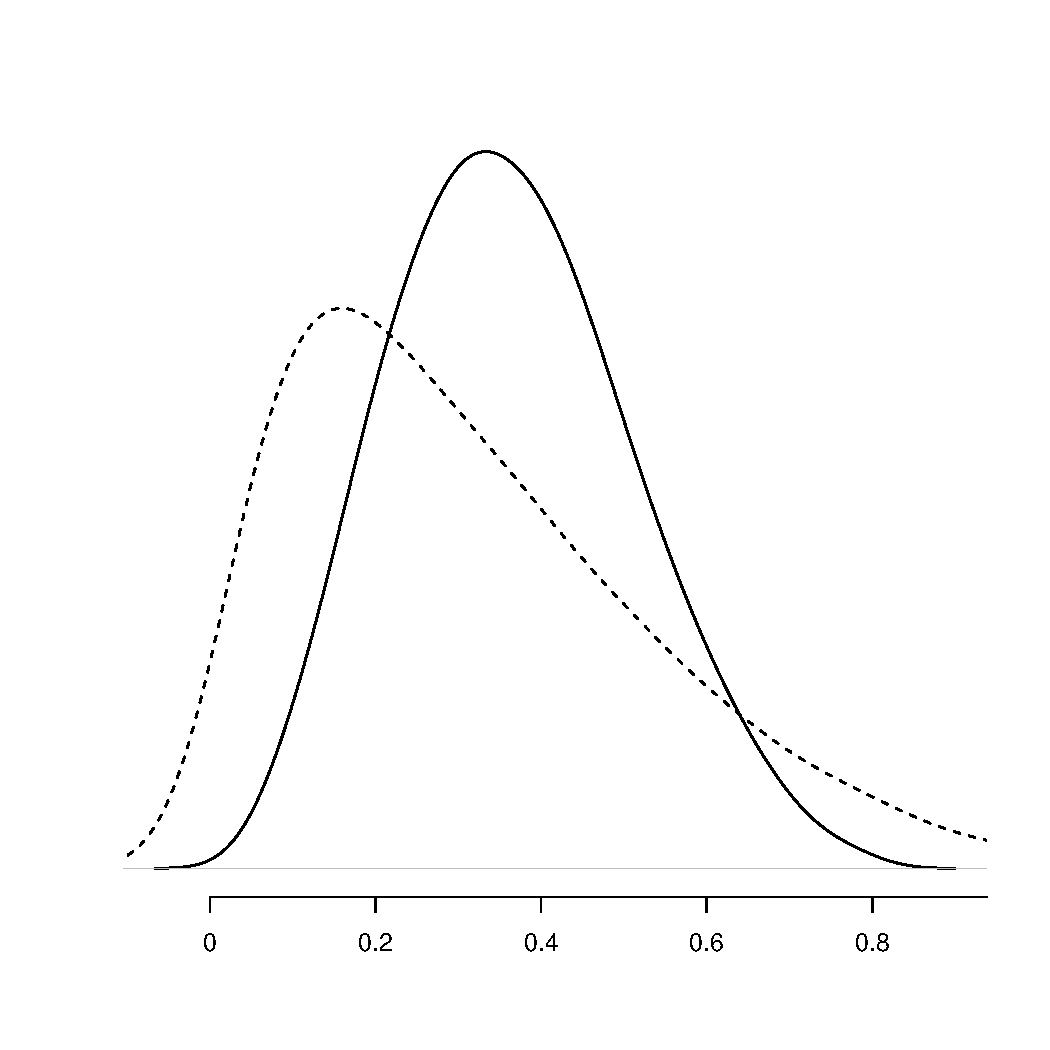
\includegraphics[width=4.05cm]{Sim_Kendall-Kruskal_4443_a.pdf} \\ 
		              Sample\_Sizes=(7,6) &   Sample\_Sizes=(5,5,5)  &    Sample\_Sizes=(4,4,4,3) \\  
\hline 
	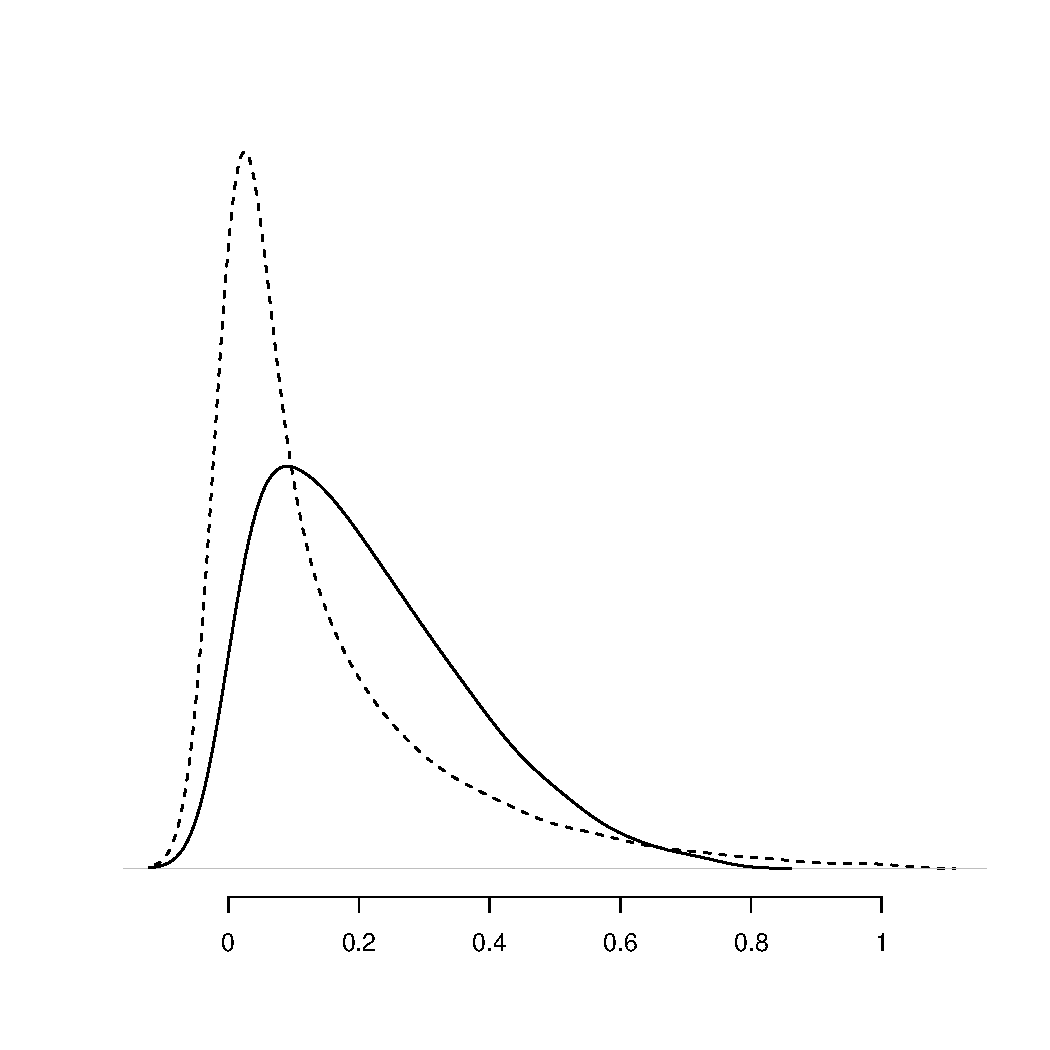
\includegraphics[width=4.05cm]{Sim_Kendall-Kruskal_1010_b.pdf} & 
		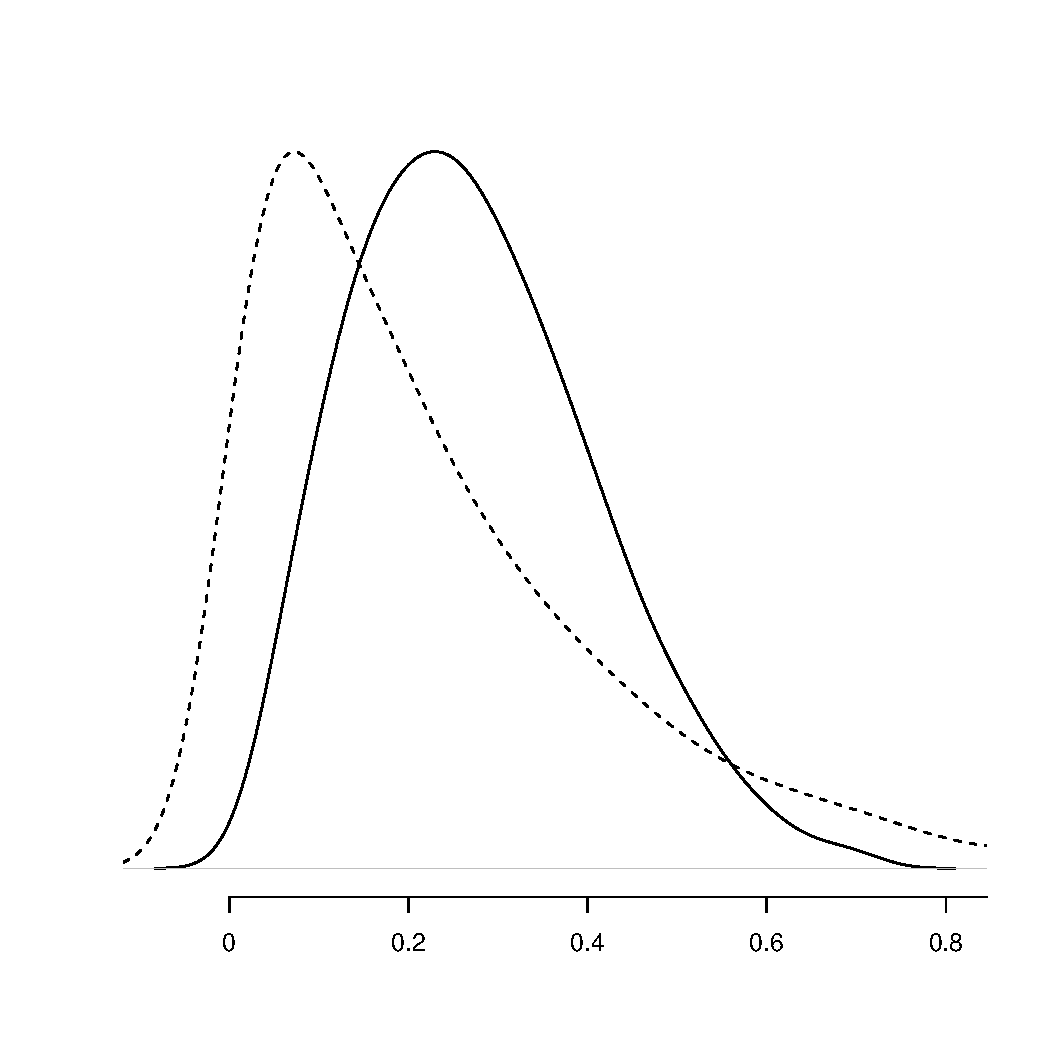
\includegraphics[width=4.05cm]{Sim_Kendall-Kruskal_776_a.pdf} & 
		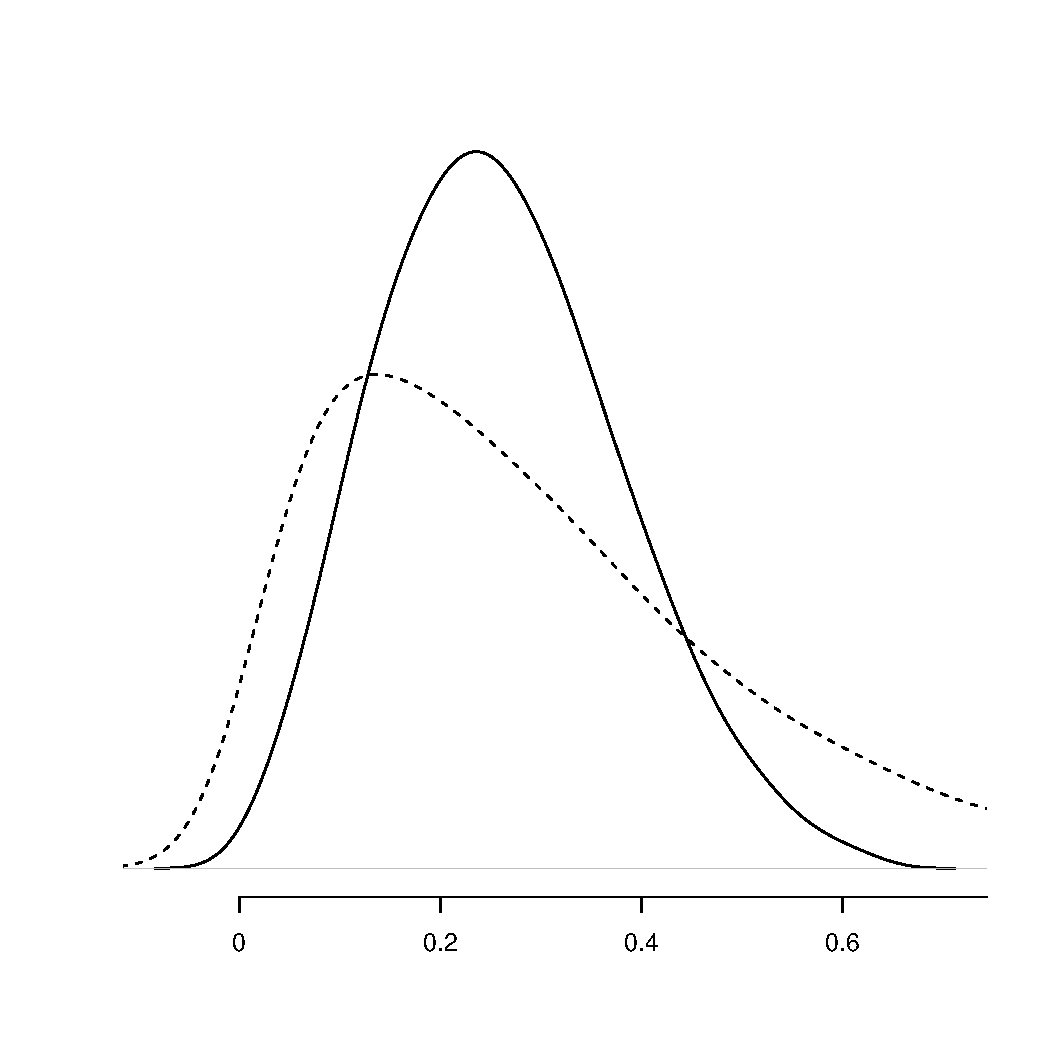
\includegraphics[width=4.05cm]{Sim_Kendall-Kruskal_5555_a.pdf} \\ 
		              Sample\_Sizes=(10,10) &   Sample\_Sizes=(7,7,6)  &    Sample\_Sizes=(5,5,5,5) \\  
\hline 
	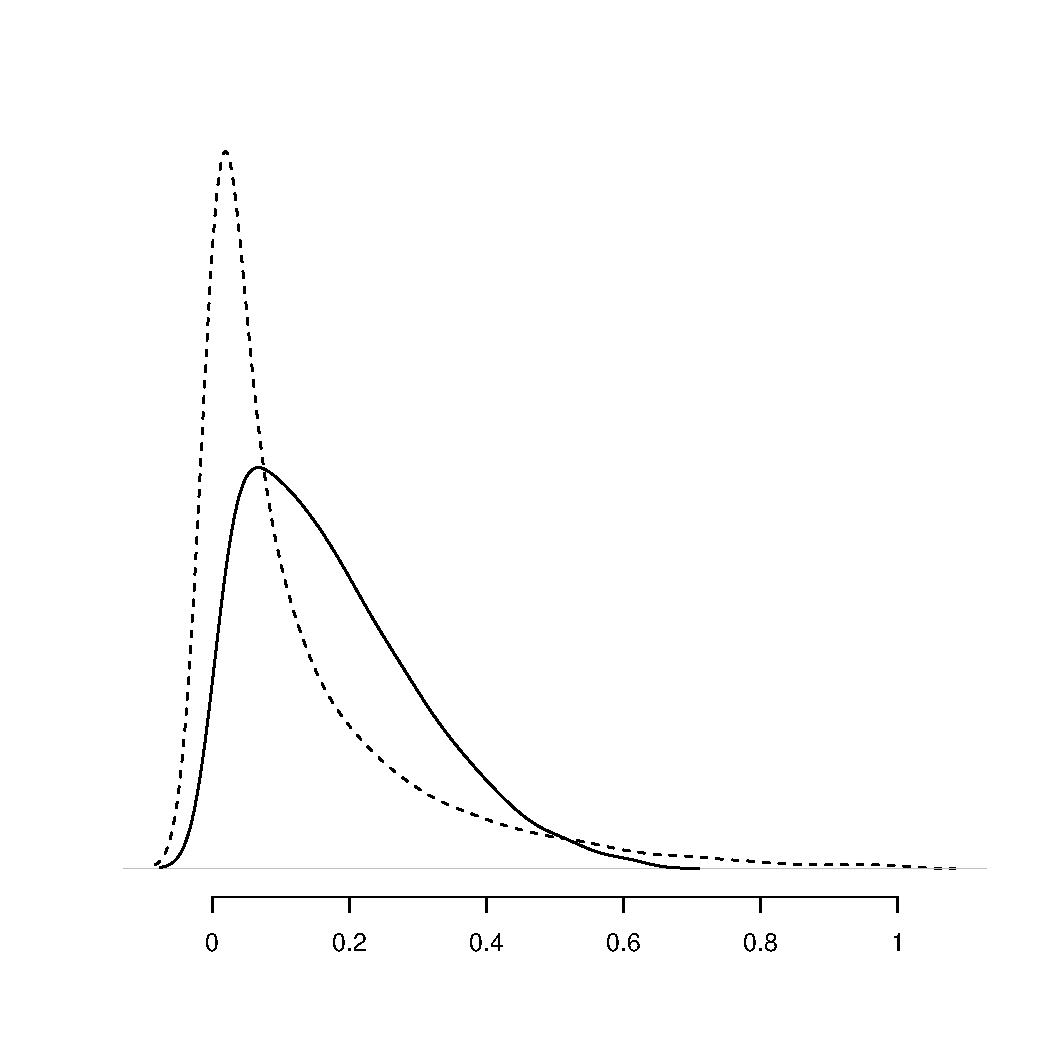
\includegraphics[width=4.05cm]{Sim_Kendall-Kruskal_1515_b.pdf} & 
		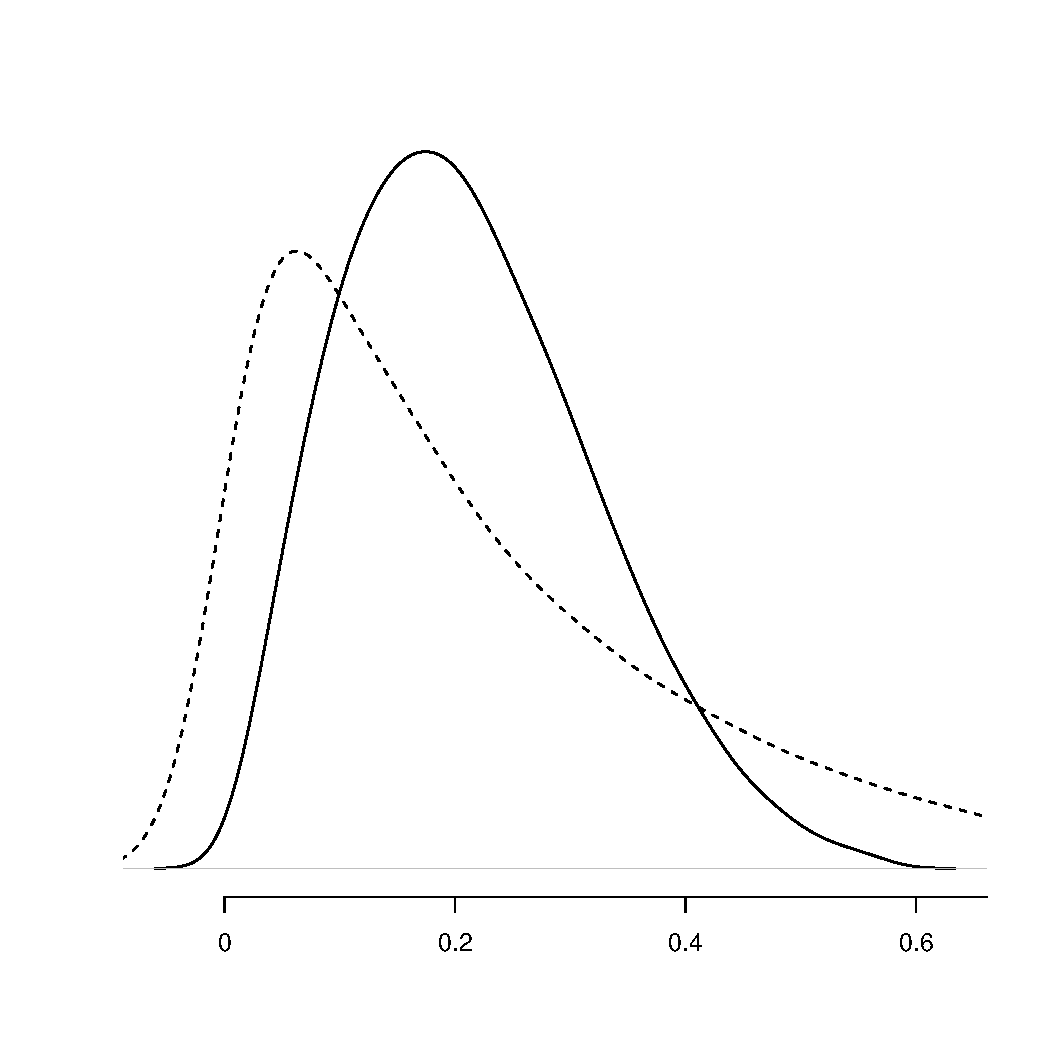
\includegraphics[width=4.05cm]{Sim_Kendall-Kruskal_101010_a.pdf} & 
		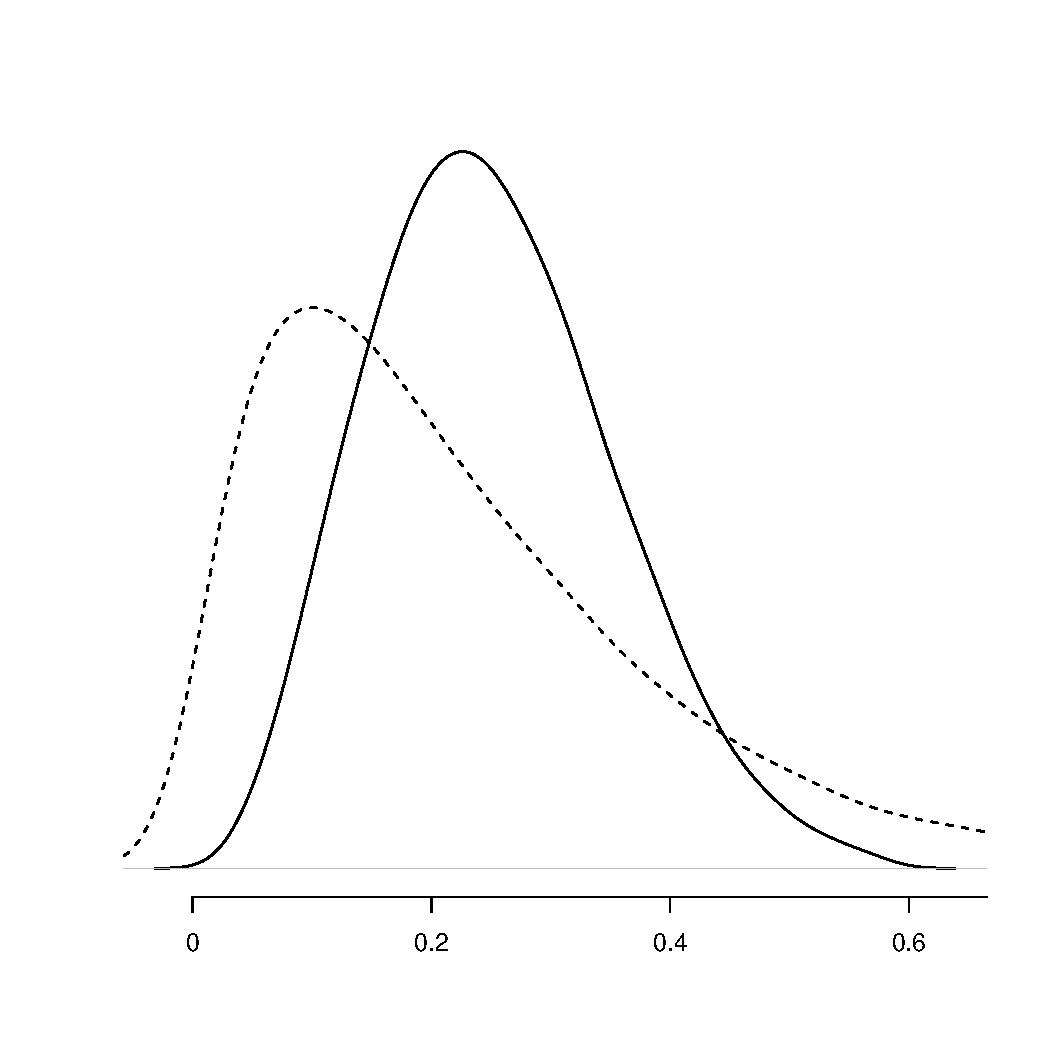
\includegraphics[width=4.05cm]{Sim_Kendall-Kruskal_8877_a.pdf} \\ 
		              Sample\_Sizes=(15,15) &   Sample\_Sizes=(10,10,10) &    Sample\_Sizes=(8,8,7,7) \\  
		              \hline

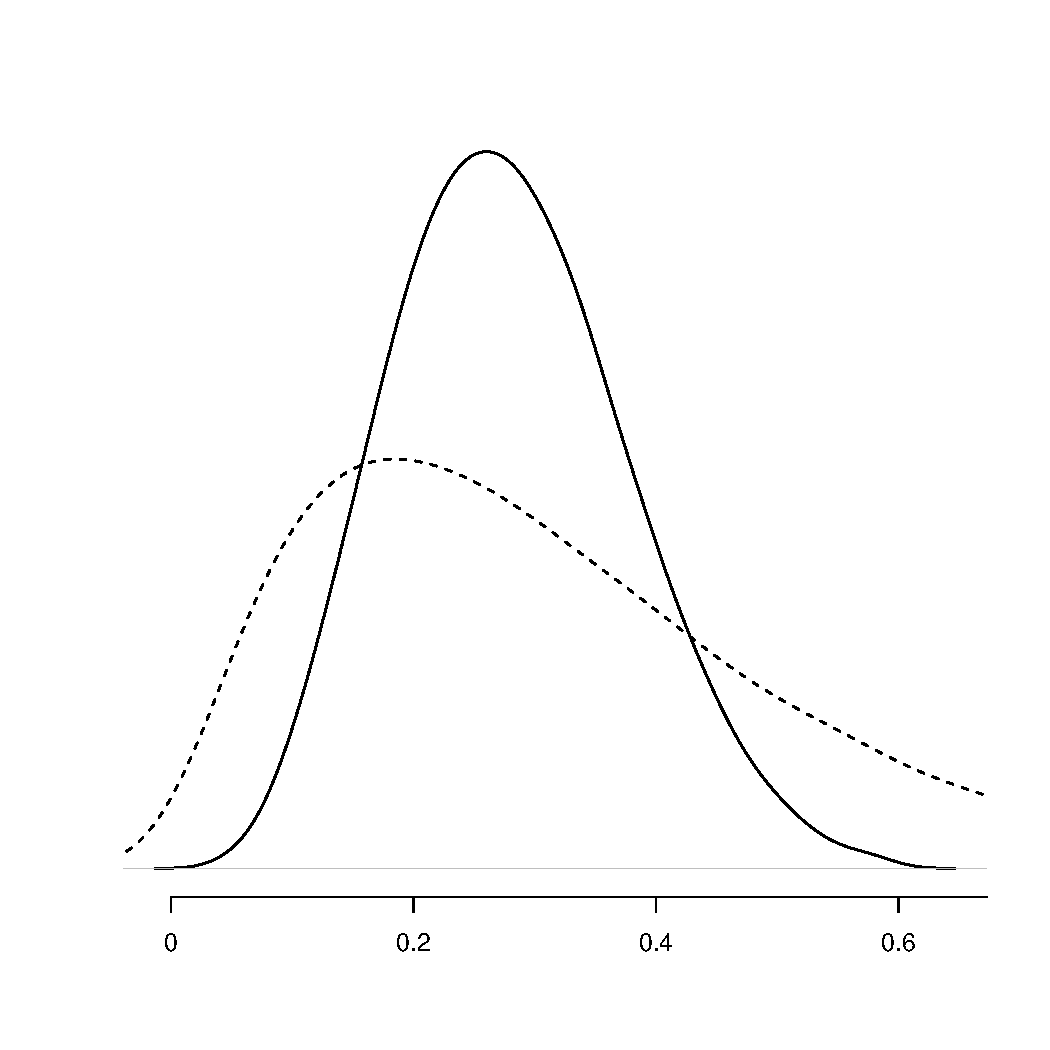
\includegraphics[width=4.05cm]{Sim_Kendall-Kruskal_66666_a.pdf} & 
		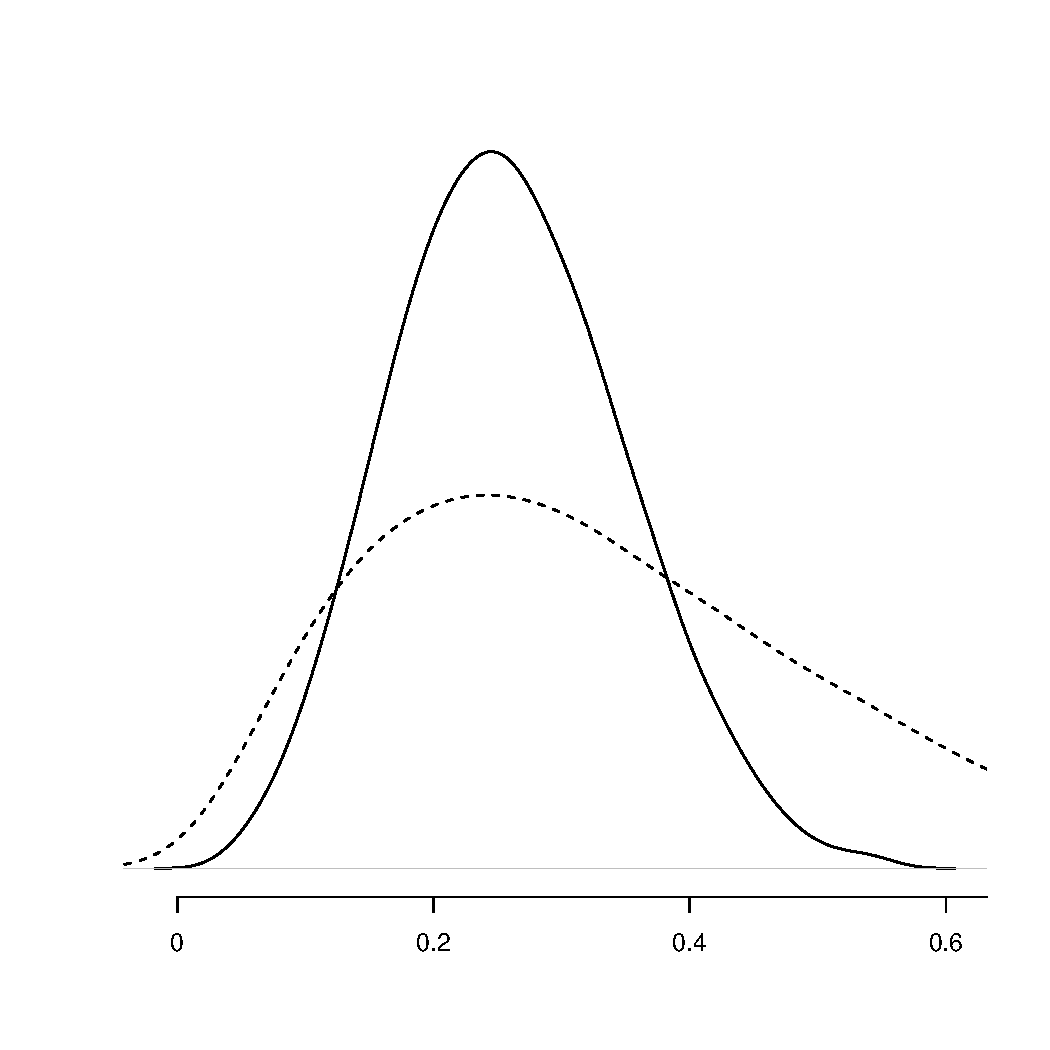
\includegraphics[width=4.05cm]{Sim_Kendall-Kruskal_555555_a.pdf} & 
		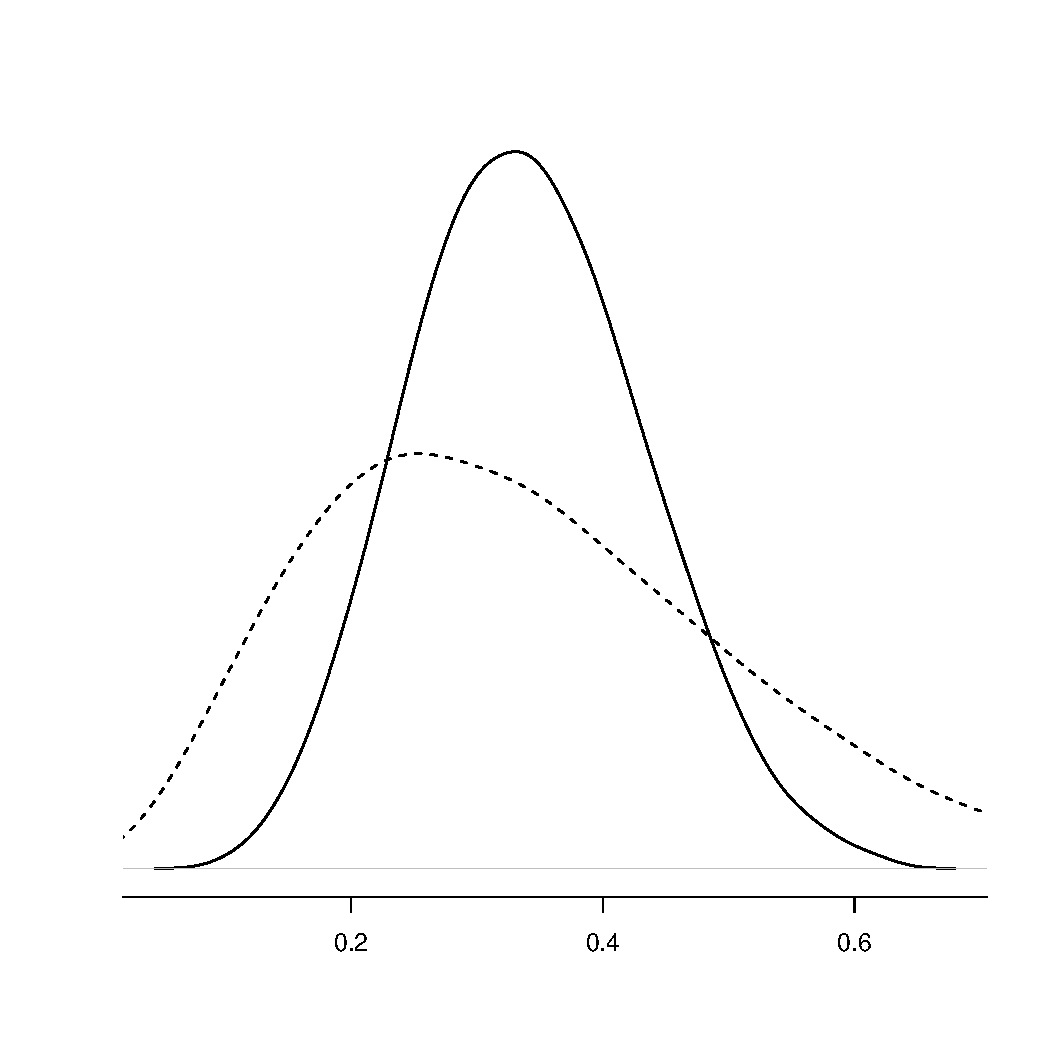
\includegraphics[width=4.05cm]{Sim_Kendall-Kruskal_5544444_a.pdf} \\ 
		              Sample\_Sizes=(6,6,6,6,6,6)  &   Sample\_Sizes=(5,5,5,5,5,5)  &    Sample\_Sizes=(5,5,4,4,4,4,4) \\  
		              \hline
\vspace{0.02cm}
\end{longtable}

\newpage

\section{Appendix C: Concordance coefficient p-values} \label{A:CCtables}

In order to compute the  probability distribution of the Concordance coefficient, the enumeration of all the permutations of elements from an order is required. Note for example that if we  have 4 samples with 6 elements each, $N=(6,6,6,6)$, the number of possible results in the experiment is $24!/6!6!6!6!$ $= 2.15433\cdot 10 ^{20}$. The total computational time to compute the Concordance coefficient for all $2.15433\cdot 10 ^{20}$ possibilities was  more than 60 days in an Intel(R) Xeon (R)   processor CPU E5-2650 v3 @ 2.30 GHz, 20 cores and RAM 64 GiB. Algorithm~\ref{alg:pvalues} presents the recursive function used to evaluate the Concordance coefficient probability distribution. 

\begin{algorithm}  \small
  \KwData{\\
  $\mathbf{p}:$ ordered array of integers  with ties.\\
  $n:$ length of $\mathbf{p}$.\\
  $Frequency[0,max(disorder)]$.}
\DontPrintSemicolon
  \SetKwFunction{FMain}{}
  \SetKwProg{Fn}{Main}{}{}
  \Fn{\FMain{$\mathbf{p}$}}{
        Permutation($\mathbf{p}$,0,$n$); \;
         \KwRet\;
  }
  \SetKwFunction{FPerm}{}
  \SetKwProg{Fn}{Permutation}{:}{}
  \Fn{\FPerm{$\mathbf{p}$,$s$,$n$}}{
         Frequency[Disorder($\mathbf{p}$)]++; \;
    	int $tmp=0$;\;
	\If{$s<n$}{
	\For{$i=n-2: \ i\geq s ;\, i--$}{
	 \For{$j=i+1;\, j<n;\, j ++$}{
	\If{$p[i]\neq p[j]$}{
	   $tmp = p[i]$;
            $p[i] = p[j]$;
            $p[j] = tmp$;
            Permutation($\mathbf{p}$,$i+1$,$n$); \;
	}
	 }
	tmp=p[i];\;
	 \For{$j=i+1;\, j<n;\, j ++$}{
	 $p[k]=p[k++]$;\;
	 }
	 $p[n-1]=tmp$;\;
	}
}
        \KwRet\;
  }
  \SetKwFunction{FDiss}{}
  \SetKwProg{Fn}{Disorder}{}{}
   \Fn{\FDiss{$\mathbf{p}$}}{
\tcc{Evaluate the disorder and the Concordance coefficient  of  permutation $\mathbf{p}$}
        \KwRet\;
  }
  	\caption{Algorithm  to compute the exact probability distribution function of the Concordance coefficient $\tau_c$ } \label{alg:pvalues}
\end{algorithm}

Tables~\ref{tablek2}, \ref{tablek3} and \ref{tablek4} show the critical values and exact p-values of the Concordance coefficient $\tau_c$ at desired significance levels of 0.10, 0.05 and 0.01 for $k$=2, $k$=3 and $k$=4 samples, respectively. 

\setlength{\tabcolsep}{1.mm}
\renewcommand{\arraystretch}{1.05}

\newpage

\footnotesize
\begin{longtable}[h]{rrrcccccccccccc} 
\endfirsthead

\multicolumn{15}{c}%
{{\bfseries \tablename\ \thetable{} -- continued from previous page}}  \\ \cline{1-15}
\hline \multicolumn{4}{c}{Sample Sizes} &  $dis$  & $\tau_c$ \, & p-value &&  $dis$  & $\tau_c$ \, & p-value &&  $dis$  & $\tau_c$ \,& p-value \\ \hline
\endhead

\hline \multicolumn{15}{r}{{Continued on next page}} \\ \hline
\caption{Critical values and exact p-values of the Concordance coefficient $\tau_c$ for $k$=2 samples.} \label{tablek2} \\
\endfoot

%\hline 
\caption{Critical values and exact p-values of the Concordance coefficient $\tau_c$ for $k$=2 samples.} 
\endlastfoot

\hline
   & &&  &  \multicolumn{3}{c}{.10} &&  \multicolumn{3}{c}{.05} &&  \multicolumn{3}{c}{.01} \\  \cline{5-7} \cline{9-11} \cline{13-15}
\multicolumn{4}{c}{Sample Sizes} &  $dis$  & $\tau_c$ \, & p-value &&  $dis$  & $\tau_c$ \, & p-value &&  $dis$  & $\tau_c$ \,& p-value \\ \hline

4	&	1	&&&		&		&		&&		&		&		&&		&		&		\\
4	&	2	&&&		&		&		&&		&		&		&&		&		&		\\
4	&	3	&&&	0	&	1.000000	&	0.057143	&&		&		&		&&		&		&		\\
4	&	4	&&&	1	&	0.875000	&	0.057143	&&	0	&	1.000000	&	0.028571	&&		&		&		\\
5	&	1	&&&		&		&		&&		&		&		&&		&		&		\\
5	&	2	&&&	0	&	1.000000	&	0.095238	&&		&		&		&&		&		&		\\
5	&	3	&&&	1	&	0.857143	&	0.071429	&&	0	&	1.000000	&	0.035714	&&		&		&		\\
5	&	4	&&&	2	&	0.800000	&	0.063492	&&	1	&	0.900000	&	0.031746	&&		&		&		\\
5	&	5	&&&	4	&	0.666667	&	0.095238	&&	2	&	0.833333	&	0.031746	&&	0	&	1.000000	&	0.007937	\\
6	&	1	&&&		&		&		&&		&		&		&&		&		&		\\
6	&	2	&&&	0	&	1.000000	&	0.071429	&&		&		&		&&		&		&		\\
6	&	3	&&&	2	&	0.777778	&	0.095238	&&	1	&	0.888889	&	0.047619	&&		&		&		\\
6	&	4	&&&	3	&	0.750000	&	0.066667	&&	2	&	0.833333	&	0.038095	&&	0	&	1.000000	&	0.009524	\\
6	&	5	&&&	5	&	0.666667	&	0.082251	&&	3	&	0.800000	&	0.030303	&&	1	&	0.933333	&	0.008658	\\
6	&	6	&&&	7	&	0.611111	&	0.093074	&&	5	&	0.722222	&	0.041126	&&	2	&	0.888889	&	0.008658	\\
7	&	1	&&&		&		&		&&		&		&		&&		&		&		\\
7	&	2	&&&	0	&	1.000000	&	0.055556	&&		&		&		&&		&		&		\\
7	&	3	&&&	2	&	0.800000	&	0.066667	&&	1	&	0.900000	&	0.033333	&&		&		&		\\
7	&	4	&&&	4	&	0.714286	&	0.072727	&&	3	&	0.785714	&	0.042424	&&	0	&	1.000000	&	0.006061	\\
7	&	5	&&&	6	&	0.647059	&	0.073232	&&	5	&	0.705882	&	0.047980	&&	1	&	0.941176	&	0.005051	\\
7	&	6	&&&	8	&	0.619048	&	0.073427	&&	6	&	0.714286	&	0.034965	&&	3	&	0.857143	&	0.008159	\\
7	&	7	&&&	11	&	0.541667	&	0.097319	&&	8	&	0.666667	&	0.037879	&&	4	&	0.833333	&	0.006993	\\
8	&	1	&&&		&		&		&&		&		&		&&		&		&		\\
8	&	2	&&&	1	&	0.875000	&	0.088889	&&	0	&	1.000000	&	0.044444	&&		&		&		\\
8	&	3	&&&	3	&	0.750000	&	0.084848	&&	2	&	0.833333	&	0.048485	&&		&		&		\\
8	&	4	&&&	5	&	0.687500	&	0.072727	&&	4	&	0.750000	&	0.048485	&&	1	&	0.937500	&	0.008081	\\
8	&	5	&&&	8	&	0.600000	&	0.093240	&&	6	&	0.700000	&	0.045066	&&	2	&	0.900000	&	0.006216	\\
8	&	6	&&&	10	&	0.583333	&	0.081252	&&	8	&	0.666667	&	0.042624	&&	4	&	0.833333	&	0.007992	\\
8	&	7	&&&	13	&	0.535714	&	0.093862	&&	10	&	0.642857	&	0.040093	&&	6	&	0.785714	&	0.009324	\\
8	&	8	&&&	15	&	0.531250	&	0.082984	&&	13	&	0.593750	&	0.049883	&&	7	&	0.781250	&	0.006993	\\
9	&	1	&&&		&		&		&&		&		&		&&		&		&		\\
9	&	2	&&&	1	&	0.888889	&	0.072727	&&	0	&	1.000000	&	0.036364	&&		&		&		\\
9	&	3	&&&	3	&	0.769231	&	0.063636	&&	2	&	0.846154	&	0.036364	&&	0	&	1.000000	&	0.009091	\\
9	&	4	&&&	6	&	0.666667	&	0.075524	&&	4	&	0.777778	&	0.033566	&&	1	&	0.944444	&	0.005594	\\
9	&	5	&&&	9	&	0.590909	&	0.082917	&&	7	&	0.681818	&	0.041958	&&	3	&	0.863636	&	0.006993	\\
9	&	6	&&&	12	&	0.555556	&	0.087912	&&	10	&	0.629630	&	0.049550	&&	5	&	0.814815	&	0.007592	\\
9	&	7	&&&	15	&	0.516129	&	0.090734	&&	12	&	0.612903	&	0.041783	&&	7	&	0.774194	&	0.007867	\\
9	&	8	&&&	18	&	0.500000	&	0.092719	&&	15	&	0.583333	&	0.046401	&&	9	&	0.750000	&	0.007898	\\
9	&	9	&&&	21	&	0.475000	&	0.093912	&&	17	&	0.575000	&	0.039984	&&	11	&	0.725000	&	0.007775	\\
10	&	1	&&&		&		&		&&		&		&		&&		&		&		\\
10	&	2	&&&	1	&	0.900000	&	0.060606	&&	0	&	1.000000	&	0.030303	&&		&		&		\\
10	&	3	&&&	4	&	0.733333	&	0.076923	&&	3	&	0.800000	&	0.048951	&&	0	&	1.000000	&	0.006993	\\
10	&	4	&&&	7	&	0.650000	&	0.075924	&&	5	&	0.750000	&	0.035964	&&	2	&	0.900000	&	0.007992	\\
10	&	5	&&&	11	&	0.560000	&	0.099234	&&	8	&	0.680000	&	0.039960	&&	4	&	0.840000	&	0.007992	\\
10	&	6	&&&	14	&	0.533333	&	0.093407	&&	11	&	0.633333	&	0.041958	&&	6	&	0.800000	&	0.007493	\\
10	&	7	&&&	17	&	0.514286	&	0.087824	&&	14	&	0.600000	&	0.043089	&&	9	&	0.742857	&	0.009667	\\
10	&	8	&&&	20	&	0.500000	&	0.083139	&&	17	&	0.575000	&	0.043421	&&	11	&	0.725000	&	0.008547	\\
10	&	9	&&&	24	&	0.466667	&	0.094720	&&	20	&	0.555556	&	0.043474	&&	13	&	0.711111	&	0.007621	\\
10	&	10	&&&	27	&	0.460000	&	0.089210	&&	23	&	0.540000	&	0.043257	&&	16	&	0.680000	&	0.008931	\\
11	&	1	&&&		&		&		&&		&		&		&&		&		&		\\
11	&	2	&&&	1	&	0.909091	&	0.051282	&&	0	&	1.000000	&	0.025641	&&		&		&		\\
11	&	3	&&&	5	&	0.687500	&	0.087912	&&	3	&	0.812500	&	0.038462	&&	0	&	1.000000	&	0.005495	\\
11	&	4	&&&	8	&	0.636364	&	0.077656	&&	6	&	0.727273	&	0.039560	&&	2	&	0.909091	&	0.005861	\\
11	&	5	&&&	12	&	0.555556	&	0.089744	&&	9	&	0.666667	&	0.038004	&&	5	&	0.814815	&	0.008700	\\
11	&	6	&&&	16	&	0.515152	&	0.098255	&&	13	&	0.606061	&	0.047673	&&	7	&	0.787879	&	0.007111	\\
11	&	7	&&&	19	&	0.500000	&	0.085344	&&	16	&	0.578947	&	0.044118	&&	10	&	0.736842	&	0.008296	\\
11	&	8	&&&	23	&	0.477273	&	0.090842	&&	19	&	0.568182	&	0.040883	&&	13	&	0.704545	&	0.009103	\\
11	&	9	&&&	27	&	0.448980	&	0.095177	&&	23	&	0.530612	&	0.046452	&&	16	&	0.673469	&	0.009693	\\
11	&	10	&&&	31	&	0.436364	&	0.098618	&&	26	&	0.527273	&	0.042964	&&	18	&	0.672727	&	0.007950	\\
11	&	11	&&&	34	&	0.433333	&	0.087946	&&	30	&	0.500000	&	0.047307	&&	21	&	0.650000	&	0.008330	\\
12	&	1	&&&		&		&		&&		&		&		&&		&		&		\\
12	&	2	&&&	2	&	0.833333	&	0.087912	&&	1	&	0.916667	&	0.043956	&&		&		&		\\
12	&	3	&&&	5	&	0.722222	&	0.070330	&&	4	&	0.777778	&	0.048352	&&	1	&	0.944444	&	0.008791	\\
12	&	4	&&&	9	&	0.625000	&	0.078022	&&	7	&	0.708333	&	0.041758	&&	3	&	0.875000	&	0.007692	\\
12	&	5	&&&	13	&	0.566667	&	0.081771	&&	11	&	0.633333	&	0.048481	&&	6	&	0.800000	&	0.009373	\\
12	&	6	&&&	17	&	0.527778	&	0.083064	&&	14	&	0.611111	&	0.041478	&&	9	&	0.750000	&	0.009696	\\
12	&	7	&&&	21	&	0.500000	&	0.083115	&&	18	&	0.571429	&	0.044931	&&	12	&	0.714286	&	0.009764	\\
12	&	8	&&&	26	&	0.458333	&	0.097880	&&	22	&	0.541667	&	0.047345	&&	15	&	0.687500	&	0.009558	\\
12	&	9	&&&	30	&	0.444444	&	0.095451	&&	26	&	0.518519	&	0.049073	&&	18	&	0.666667	&	0.009288	\\
12	&	10	&&&	34	&	0.433333	&	0.093090	&&	29	&	0.516667	&	0.042570	&&	21	&	0.650000	&	0.008957	\\
12	&	11	&&&	38	&	0.424242	&	0.090842	&&	33	&	0.500000	&	0.043879	&&	24	&	0.636364	&	0.008625	\\
12	&	12	&&&	42	&	0.416667	&	0.088734	&&	37	&	0.486111	&	0.044902	&&	27	&	0.625000	&	0.008293	\\
13	&	1	&&&		&		&		&&		&		&		&&		&		&		\\
13	&	2	&&&	2	&	0.846154	&	0.076190	&&	1	&	0.923077	&	0.038095	&&		&		&		\\
13	&	3	&&&	6	&	0.684211	&	0.082143	&&	4	&	0.789474	&	0.039286	&&	1	&	0.947368	&	0.007143	\\
13	&	4	&&&	10	&	0.615385	&	0.078992	&&	8	&	0.692308	&	0.044538	&&	3	&	0.884615	&	0.005882	\\
13	&	5	&&&	15	&	0.531250	&	0.094538	&&	12	&	0.625000	&	0.045985	&&	7	&	0.781250	&	0.009804	\\
13	&	6	&&&	19	&	0.512820	&	0.087424	&&	16	&	0.589744	&	0.046218	&&	10	&	0.743590	&	0.009214	\\
13	&	7	&&&	24	&	0.466667	&	0.096801	&&	20	&	0.555556	&	0.045562	&&	13	&	0.711111	&	0.008462	\\
13	&	8	&&&	28	&	0.461538	&	0.089046	&&	24	&	0.538462	&	0.044553	&&	17	&	0.673077	&	0.009937	\\
13	&	9	&&&	33	&	0.431035	&	0.095557	&&	28	&	0.517241	&	0.043376	&&	20	&	0.655172	&	0.008910	\\
13	&	10	&&&	37	&	0.430769	&	0.088294	&&	33	&	0.492308	&	0.049329	&&	24	&	0.630769	&	0.009888	\\
13	&	11	&&&	42	&	0.408451	&	0.093307	&&	37	&	0.478873	&	0.047448	&&	27	&	0.619718	&	0.008848	\\
13	&	12	&&&	47	&	0.397436	&	0.097642	&&	41	&	0.474359	&	0.045711	&&	31	&	0.602564	&	0.009556	\\
13	&	13	&&&	51	&	0.392857	&	0.090847	&&	45	&	0.464286	&	0.044117	&&	34	&	0.595238	&	0.008601	\\
14	&	1	&&&		&		&		&&		&		&		&&		&		&		\\
14	&	2	&&&	2	&	0.857143	&	0.066667	&&	1	&	0.928571	&	0.033333	&&		&		&		\\
14	&	3	&&&	7	&	0.666667	&	0.091176	&&	5	&	0.761905	&	0.047059	&&	1	&	0.952381	&	0.005882	\\
14	&	4	&&&	11	&	0.607143	&	0.079085	&&	9	&	0.678571	&	0.046405	&&	4	&	0.857143	&	0.007843	\\
14	&	5	&&&	16	&	0.542857	&	0.087031	&&	13	&	0.628571	&	0.043688	&&	7	&	0.800000	&	0.007224	\\
14	&	6	&&&	21	&	0.500000	&	0.091331	&&	17	&	0.595238	&	0.040764	&&	11	&	0.738095	&	0.008720	\\
14	&	7	&&&	26	&	0.469388	&	0.093774	&&	22	&	0.551020	&	0.046096	&&	15	&	0.693878	&	0.009684	\\
14	&	8	&&&	31	&	0.446429	&	0.095018	&&	26	&	0.535714	&	0.042149	&&	18	&	0.678571	&	0.008125	\\
14	&	9	&&&	36	&	0.428571	&	0.095574	&&	31	&	0.507936	&	0.045585	&&	22	&	0.650794	&	0.008568	\\
14	&	10	&&&	41	&	0.414286	&	0.095643	&&	36	&	0.485714	&	0.048404	&&	26	&	0.628571	&	0.008851	\\
14	&	11	&&&	46	&	0.402597	&	0.095427	&&	40	&	0.480519	&	0.044228	&&	30	&	0.610390	&	0.009022	\\
14	&	12	&&&	51	&	0.392857	&	0.095012	&&	45	&	0.464286	&	0.046354	&&	34	&	0.595238	&	0.009114	\\
14	&	13	&&&	56	&	0.384615	&	0.094479	&&	50	&	0.450549	&	0.048173	&&	38	&	0.582418	&	0.009150	\\
14	&	14	&&&	61	&	0.377551	&	0.093868	&&	55	&	0.438776	&	0.049736	&&	42	&	0.571429	&	0.009146	\\
15	&	1	&&&		&		&		&&		&		&		&&		&		&		\\
15	&	2	&&&	3	&	0.800000	&	0.088235	&&	1	&	0.933333	&	0.029412	&&		&		&		\\
15	&	3	&&&	7	&	0.681818	&	0.075980	&&	5	&	0.772727	&	0.039216	&&	2	&	0.909091	&	0.009804	\\
15	&	4	&&&	12	&	0.600000	&	0.079979	&&	10	&	0.666667	&	0.048504	&&	5	&	0.833333	&	0.009288	\\
15	&	5	&&&	18	&	0.513514	&	0.098297	&&	14	&	0.621622	&	0.041796	&&	8	&	0.783784	&	0.007740	\\
15	&	6	&&&	23	&	0.488889	&	0.094833	&&	19	&	0.577778	&	0.044855	&&	12	&	0.733333	&	0.008367	\\
15	&	7	&&&	28	&	0.461538	&	0.091085	&&	24	&	0.538462	&	0.046522	&&	16	&	0.692308	&	0.008526	\\
15	&	8	&&&	33	&	0.450000	&	0.087332	&&	29	&	0.516667	&	0.047304	&&	20	&	0.666667	&	0.008456	\\
15	&	9	&&&	39	&	0.417910	&	0.095507	&&	34	&	0.492537	&	0.047584	&&	24	&	0.641791	&	0.008255	\\
15	&	10	&&&	44	&	0.413333	&	0.090971	&&	39	&	0.480000	&	0.047524	&&	29	&	0.613333	&	0.009616	\\
15	&	11	&&&	50	&	0.390244	&	0.097262	&&	44	&	0.463415	&	0.047262	&&	33	&	0.597561	&	0.009154	\\
15	&	12	&&&	55	&	0.388889	&	0.092610	&&	49	&	0.455556	&	0.046866	&&	37	&	0.588889	&	0.008710	\\
15	&	13	&&&	61	&	0.371134	&	0.097721	&&	54	&	0.443299	&	0.046394	&&	42	&	0.567010	&	0.009635	\\
15	&	14	&&&	66	&	0.371429	&	0.093216	&&	59	&	0.438095	&	0.045875	&&	46	&	0.561905	&	0.009115	\\
15	&	15	&&&	72	&	0.357143	&	0.097526	&&	64	&	0.428571	&	0.045334	&&	51	&	0.544643	&	0.009875	\\
16	&	1	&&&		&		&		&&		&		&		&&		&		&		\\
16	&	2	&&&	3	&	0.812500	&	0.078431	&&	1	&	0.937500	&	0.026144	&&		&		&		\\
16	&	3	&&&	8	&	0.666667	&	0.084623	&&	6	&	0.750000	&	0.047472	&&	2	&	0.916667	&	0.008256	\\
16	&	4	&&&	14	&	0.562500	&	0.099484	&&	11	&	0.656250	&	0.049948	&&	5	&	0.843750	&	0.007430	\\
16	&	5	&&&	19	&	0.525000	&	0.091012	&&	15	&	0.625000	&	0.040100	&&	9	&	0.775000	&	0.008158	\\
16	&	6	&&&	25	&	0.479167	&	0.098026	&&	21	&	0.562500	&	0.048731	&&	13	&	0.729167	&	0.007988	\\
16	&	7	&&&	30	&	0.464286	&	0.088694	&&	26	&	0.535714	&	0.046876	&&	18	&	0.678571	&	0.009578	\\
16	&	8	&&&	36	&	0.437500	&	0.092602	&&	31	&	0.515625	&	0.044823	&&	22	&	0.656250	&	0.008748	\\
16	&	9	&&&	42	&	0.416667	&	0.095397	&&	37	&	0.486111	&	0.049384	&&	27	&	0.625000	&	0.009643	\\
16	&	10	&&&	48	&	0.400000	&	0.097414	&&	42	&	0.475000	&	0.046707	&&	31	&	0.612500	&	0.008685	\\
16	&	11	&&&	54	&	0.386364	&	0.098866	&&	47	&	0.465909	&	0.044271	&&	36	&	0.590909	&	0.009256	\\
16	&	12	&&&	60	&	0.375000	&	0.099904	&&	53	&	0.447917	&	0.047276	&&	41	&	0.572917	&	0.009707	\\
16	&	13	&&&	65	&	0.375000	&	0.091611	&&	59	&	0.432692	&	0.049924	&&	45	&	0.567308	&	0.008738	\\
16	&	14	&&&	71	&	0.366071	&	0.092540	&&	64	&	0.428571	&	0.047205	&&	50	&	0.553571	&	0.009064	\\
16	&	15	&&&	77	&	0.358333	&	0.093259	&&	70	&	0.416667	&	0.049381	&&	55	&	0.541667	&	0.009331	\\
16	&	16	&&&	83	&	0.351562	&	0.093812	&&	75	&	0.414062	&	0.046815	&&	60	&	0.531250	&	0.009551	\\
17	&	1	&&&		&		&		&&		&		&		&&		&		&		\\
17	&	2	&&&	3	&	0.823529	&	0.070175	&&	2	&	0.882353	&	0.046784	&&		&		&		\\
17	&	3	&&&	9	&	0.640000	&	0.092982	&&	6	&	0.760000	&	0.040351	&&	2	&	0.920000	&	0.007018	\\
17	&	4	&&&	15	&	0.558824	&	0.098580	&&	11	&	0.676471	&	0.040434	&&	6	&	0.823529	&	0.009023	\\
17	&	5	&&&	20	&	0.523810	&	0.084909	&&	17	&	0.595238	&	0.047695	&&	10	&	0.761905	&	0.008582	\\
17	&	6	&&&	26	&	0.490196	&	0.086501	&&	22	&	0.568627	&	0.043766	&&	15	&	0.705882	&	0.009867	\\
17	&	7	&&&	33	&	0.440678	&	0.099490	&&	28	&	0.525424	&	0.047171	&&	19	&	0.677966	&	0.008518	\\
17	&	8	&&&	39	&	0.426471	&	0.097491	&&	34	&	0.500000	&	0.049474	&&	24	&	0.647059	&	0.009005	\\
17	&	9	&&&	45	&	0.407895	&	0.095246	&&	39	&	0.486842	&	0.044566	&&	29	&	0.618421	&	0.009248	\\
17	&	10	&&&	51	&	0.400000	&	0.092922	&&	45	&	0.470588	&	0.045937	&&	34	&	0.600000	&	0.009341	\\
17	&	11	&&&	57	&	0.387097	&	0.090623	&&	51	&	0.451613	&	0.046916	&&	39	&	0.580645	&	0.009331	\\
17	&	12	&&&	64	&	0.372549	&	0.097270	&&	57	&	0.441176	&	0.047604	&&	44	&	0.568627	&	0.009257	\\
17	&	13	&&&	70	&	0.363636	&	0.094466	&&	63	&	0.427273	&	0.048075	&&	49	&	0.554545	&	0.009141	\\
17	&	14	&&&	77	&	0.352941	&	0.099995	&&	69	&	0.420168	&	0.048385	&&	54	&	0.546219	&	0.008999	\\
17	&	15	&&&	83	&	0.346457	&	0.096996	&&	75	&	0.409449	&	0.048571	&&	60	&	0.527559	&	0.009973	\\
17	&	16	&&&	89	&	0.345588	&	0.094235	&&	81	&	0.404412	&	0.048664	&&	65	&	0.522059	&	0.009731	\\
17	&	17	&&&	96	&	0.333333	&	0.098687	&&	87	&	0.395833	&	0.048686	&&	70	&	0.513889	&	0.009494	\\
18	&	1	&&&		&		&		&&		&		&		&&		&		&		\\
18	&	2	&&&	4	&	0.777778	&	0.094737	&&	2	&	0.888889	&	0.042105	&&		&		&		\\
18	&	3	&&&	9	&	0.666667	&	0.079699	&&	7	&	0.740741	&	0.046617	&&	2	&	0.925926	&	0.006015	\\
18	&	4	&&&	16	&	0.555556	&	0.098154	&&	12	&	0.666667	&	0.042379	&&	6	&	0.833333	&	0.007382	\\
18	&	5	&&&	22	&	0.511111	&	0.094327	&&	18	&	0.600000	&	0.045707	&&	11	&	0.755556	&	0.008916	\\
18	&	6	&&&	28	&	0.481481	&	0.089527	&&	24	&	0.555556	&	0.047193	&&	16	&	0.703704	&	0.009421	\\
18	&	7	&&&	35	&	0.444444	&	0.096701	&&	30	&	0.523810	&	0.047418	&&	21	&	0.666667	&	0.009445	\\
18	&	8	&&&	41	&	0.430556	&	0.090496	&&	36	&	0.500000	&	0.046988	&&	26	&	0.638889	&	0.009233	\\
18	&	9	&&&	48	&	0.407407	&	0.095074	&&	42	&	0.481481	&	0.046198	&&	31	&	0.617284	&	0.008893	\\
18	&	10	&&&	55	&	0.388889	&	0.098664	&&	48	&	0.466667	&	0.045221	&&	37	&	0.588889	&	0.009955	\\
18	&	11	&&&	61	&	0.383838	&	0.092197	&&	55	&	0.444444	&	0.049392	&&	42	&	0.575758	&	0.009388	\\
18	&	12	&&&	68	&	0.370370	&	0.094866	&&	61	&	0.435185	&	0.047865	&&	47	&	0.564815	&	0.008851	\\
18	&	13	&&&	75	&	0.358974	&	0.097070	&&	67	&	0.427350	&	0.046401	&&	53	&	0.547009	&	0.009505	\\
18	&	14	&&&	82	&	0.349206	&	0.098905	&&	74	&	0.412698	&	0.049436	&&	58	&	0.539683	&	0.008925	\\
18	&	15	&&&	88	&	0.348148	&	0.092994	&&	80	&	0.407407	&	0.047795	&&	64	&	0.525926	&	0.009432	\\
18	&	16	&&&	95	&	0.340278	&	0.094552	&&	86	&	0.402778	&	0.046272	&&	70	&	0.513889	&	0.009880	\\
18	&	17	&&&	102	&	0.333333	&	0.095895	&&	93	&	0.392157	&	0.048652	&&	75	&	0.509804	&	0.009265	\\
18	&	18	&&&	109	&	0.327160	&	0.097059	&&	99	&	0.388889	&	0.047085	&&	81	&	0.500000	&	0.009631	\\
19	&	1	&&&		&		&		&&		&		&		&&		&		&		\\
19	&	2	&&&	4	&	0.789474	&	0.085714	&&	2	&	0.894737	&	0.038095	&&	0	&	1.000000	&	0.009524	\\
19	&	3	&&&	10	&	0.642857	&	0.087013	&&	7	&	0.750000	&	0.040260	&&	3	&	0.892857	&	0.009091	\\
19	&	4	&&&	17	&	0.552632	&	0.097346	&&	13	&	0.657895	&	0.043817	&&	7	&	0.815789	&	0.008583	\\
19	&	5	&&&	23	&	0.510638	&	0.088368	&&	19	&	0.595745	&	0.043902	&&	12	&	0.744681	&	0.009270	\\
19	&	6	&&&	30	&	0.473684	&	0.092321	&&	25	&	0.561404	&	0.042778	&&	17	&	0.701754	&	0.009001	\\
19	&	7	&&&	37	&	0.439394	&	0.094199	&&	32	&	0.515152	&	0.047622	&&	22	&	0.666667	&	0.008489	\\
19	&	8	&&&	44	&	0.421053	&	0.094915	&&	38	&	0.500000	&	0.044792	&&	28	&	0.631579	&	0.009436	\\
19	&	9	&&&	51	&	0.400000	&	0.094882	&&	45	&	0.470588	&	0.047700	&&	33	&	0.611765	&	0.008572	\\
19	&	10	&&&	58	&	0.389474	&	0.094392	&&	52	&	0.452632	&	0.049957	&&	39	&	0.589474	&	0.009074	\\
19	&	11	&&&	65	&	0.375000	&	0.093614	&&	58	&	0.442308	&	0.046502	&&	45	&	0.567308	&	0.009429	\\
19	&	12	&&&	72	&	0.368421	&	0.092664	&&	65	&	0.429825	&	0.048074	&&	51	&	0.552632	&	0.009674	\\
19	&	13	&&&	80	&	0.349594	&	0.099454	&&	72	&	0.414634	&	0.049346	&&	57	&	0.536585	&	0.009835	\\
19	&	14	&&&	87	&	0.345865	&	0.097861	&&	78	&	0.413534	&	0.046065	&&	63	&	0.526316	&	0.009935	\\
19	&	15	&&&	94	&	0.338028	&	0.096301	&&	85	&	0.401408	&	0.047054	&&	69	&	0.514085	&	0.009986	\\
19	&	16	&&&	101	&	0.335526	&	0.094785	&&	92	&	0.394737	&	0.047883	&&	74	&	0.513158	&	0.009009	\\
19	&	17	&&&	109	&	0.322981	&	0.099827	&&	99	&	0.385093	&	0.048578	&&	81	&	0.496894	&	0.009991	\\
19	&	18	&&&	116	&	0.321637	&	0.098072	&&	106	&	0.380117	&	0.049163	&&	87	&	0.491228	&	0.009960	\\
19	&	19	&&&	123	&	0.316667	&	0.096409	&&	113	&	0.372222	&	0.049656	&&	93	&	0.483333	&	0.009914	\\
20	&	1	&&&	0	&	1.000000	&	0.095238	&&		&		&		&&		&		&		\\
20	&	2	&&&	4	&	0.800000	&	0.077922	&&	2	&	0.900000	&	0.034632	&&	0	&	1.000000	&	0.008658	\\
20	&	3	&&&	11	&	0.633333	&	0.093732	&&	8	&	0.733333	&	0.046302	&&	3	&	0.900000	&	0.007905	\\
20	&	4	&&&	18	&	0.550000	&	0.096932	&&	14	&	0.650000	&	0.045360	&&	8	&	0.800000	&	0.009976	\\
20	&	5	&&&	25	&	0.500000	&	0.096970	&&	20	&	0.600000	&	0.042349	&&	13	&	0.740000	&	0.009561	\\
20	&	6	&&&	32	&	0.466667	&	0.094905	&&	27	&	0.550000	&	0.045858	&&	18	&	0.700000	&	0.008652	\\
20	&	7	&&&	39	&	0.442857	&	0.091932	&&	34	&	0.514286	&	0.047798	&&	24	&	0.657143	&	0.009315	\\
20	&	8	&&&	47	&	0.412500	&	0.099062	&&	41	&	0.487500	&	0.048749	&&	30	&	0.625000	&	0.009617	\\
20	&	9	&&&	54	&	0.400000	&	0.094682	&&	48	&	0.466667	&	0.049091	&&	36	&	0.600000	&	0.009687	\\
20	&	10	&&&	62	&	0.380000	&	0.099577	&&	55	&	0.450000	&	0.049031	&&	42	&	0.580000	&	0.009616	\\
20	&	11	&&&	69	&	0.372727	&	0.094896	&&	62	&	0.436364	&	0.048718	&&	48	&	0.563636	&	0.009458	\\
20	&	12	&&&	77	&	0.358333	&	0.098543	&&	69	&	0.425000	&	0.048240	&&	54	&	0.550000	&	0.009249	\\
20	&	13	&&&	84	&	0.353846	&	0.093978	&&	76	&	0.415385	&	0.047661	&&	60	&	0.538462	&	0.009012	\\
20	&	14	&&&	92	&	0.342857	&	0.096865	&&	83	&	0.407143	&	0.047021	&&	67	&	0.521429	&	0.009796	\\
20	&	15	&&&	100	&	0.333333	&	0.099377	&&	90	&	0.400000	&	0.046348	&&	73	&	0.513333	&	0.009462	\\
20	&	16	&&&	107	&	0.331250	&	0.094950	&&	98	&	0.387500	&	0.049370	&&	79	&	0.506250	&	0.009140	\\
20	&	17	&&&	115	&	0.323529	&	0.097069	&&	105	&	0.382353	&	0.048471	&&	86	&	0.494118	&	0.009721	\\
20	&	18	&&&	123	&	0.316667	&	0.098957	&&	112	&	0.377778	&	0.047600	&&	92	&	0.488889	&	0.009363	\\
20	&	19	&&&	130	&	0.315789	&	0.094835	&&	119	&	0.373684	&	0.046761	&&	99	&	0.478947	&	0.009856	\\
20	&	20	&&&	138	&	0.310000	&	0.096500	&&	127	&	0.365000	&	0.049090	&&	105	&	0.475000	&	0.009484	\\ \hline
\vspace{0.02cm}
\end{longtable}


%\newpage

\begin{longtable}[h]{rrrccccccccccccc}%\scriptsize
\endfirsthead

\multicolumn{16}{c}%
{{\bfseries \tablename\ \thetable{} -- continued from previous page}}  \\ \cline{1-16}
\hline \multicolumn{5}{c}{Sample Sizes} &  $dis$  & $\tau_c$ \, & p-value &&  $dis$  & $\tau_c$ \, & p-value &&  $dis$  & $\tau_c$ \,& p-value \\ \hline
\endhead

\hline \multicolumn{16}{r}{{Continued on next page}} \\ \hline
\caption{Critical values and exact p-values of the Concordance coefficient $\tau_c$ for $k$=3 samples.} \label{tablek3} \\ 
\endfoot

%\hline 
\caption{Critical values and exact p-values of the Concordance coefficient $\tau_c$ for $k$=3 samples.}
\endlastfoot
\hline

   & && & &  \multicolumn{3}{c}{.10} &&  \multicolumn{3}{c}{.05} &&  \multicolumn{3}{c}{.01} \\  \cline{6-8} \cline{10-12} \cline{14-16}
\multicolumn{5}{c}{Sample Sizes} &  $dis$  & $\tau_c$ \, & p-value &&  $dis$  & $\tau_c$ \, & p-value &&  $dis$  & $\tau_c$ \,& p-value \\ \hline
2	&	1	&	1	&&&		&		&		&&		&		&		&&		&		&		\\
2	&	2	&	1	&&&		&		&		&&		&		&		&&		&		&		\\
2	&	2	&	2	&&&	0	&	1.000000	&	0.066667	&&		&		&		&&		&		&		\\
3	&	1	&	1	&&&		&		&		&&		&		&		&&		&		&		\\
3	&	2	&	1	&&&		&		&		&&		&		&		&&		&		&		\\
3	&	2	&	2	&&&	1	&	0.875000	&	0.085714	&&	0	&	1.000000	&	0.028571	&&		&		&		\\
3	&	3	&	1	&&&	0	&	1.000000	&	0.042857	&&	0	&	1.000000	&	0.042857	&&		&		&		\\
3	&	3	&	2	&&&	2	&	0.800000	&	0.085714	&&	1	&	0.900000	&	0.032143	&&		&		&		\\
3	&	3	&	3	&&&	3	&	0.769231	&	0.064286	&&	2	&	0.846154	&	0.028571	&&	0	&	1.000000	&	0.003571	\\
4	&	1	&	1	&&&		&		&		&&		&		&		&&		&		&		\\
4	&	2	&	1	&&&	0	&	1.000000	&	0.057143	&&		&		&		&&		&		&		\\
4	&	2	&	2	&&&	1	&	0.900000	&	0.042857	&&	1	&	0.900000	&	0.042857	&&		&		&		\\
4	&	3	&	1	&&&	1	&	0.888889	&	0.064286	&&	0	&	1.000000	&	0.021429	&&		&		&		\\
4	&	3	&	2	&&&	3	&	0.769231	&	0.077778	&&	2	&	0.846154	&	0.038095	&&	0	&	1.000000	&	0.004762	\\
4	&	3	&	3	&&&	5	&	0.687500	&	0.090000	&&	3	&	0.812500	&	0.025714	&&	1	&	0.937500	&	0.004286	\\
4	&	4	&	1	&&&	2	&	0.833333	&	0.060317	&&	1	&	0.916667	&	0.028571	&&	0	&	1.000000	&	0.009524	\\
4	&	4	&	2	&&&	4	&	0.750000	&	0.060952	&&	3	&	0.812500	&	0.032381	&&	1	&	0.937500	&	0.005714	\\
4	&	4	&	3	&&&	7	&	0.650000	&	0.095065	&&	5	&	0.750000	&	0.035325	&&	3	&	0.850000	&	0.009351	\\
4	&	4	&	4	&&&	9	&	0.625000	&	0.086580	&&	7	&	0.708333	&	0.036883	&&	4	&	0.833333	&	0.006580	\\
5	&	1	&	1	&&&		&		&		&&		&		&		&&		&		&		\\
5	&	2	&	1	&&&	1	&	0.875000	&	0.095238	&&	0	&	1.000000	&	0.035714	&&		&		&		\\
5	&	2	&	2	&&&	2	&	0.833333	&	0.058201	&&	1	&	0.916667	&	0.023810	&&	0	&	1.000000	&	0.007937	\\
5	&	3	&	1	&&&	2	&	0.818182	&	0.075397	&&	1	&	0.909091	&	0.035714	&&		&		&		\\
5	&	3	&	2	&&&	4	&	0.733333	&	0.072222	&&	3	&	0.800000	&	0.038889	&&	1	&	0.933333	&	0.007143	\\
5	&	3	&	3	&&&	6	&	0.684211	&	0.070130	&&	5	&	0.736842	&	0.041558	&&	2	&	0.894737	&	0.005195	\\
5	&	4	&	1	&&&	4	&	0.714286	&	0.098413	&&	2	&	0.857143	&	0.031746	&&	0	&	1.000000	&	0.004762	\\
5	&	4	&	2	&&&	6	&	0.684211	&	0.079654	&&	5	&	0.736842	&	0.049062	&&	2	&	0.894737	&	0.006926	\\
5	&	4	&	3	&&&	9	&	0.608696	&	0.098341	&&	7	&	0.695652	&	0.042641	&&	4	&	0.826087	&	0.008009	\\
5	&	4	&	4	&&&	11	&	0.607143	&	0.079343	&&	9	&	0.678571	&	0.037163	&&	6	&	0.785714	&	0.008658	\\
5	&	5	&	1	&&&	5	&	0.705882	&	0.077201	&&	4	&	0.764706	&	0.047619	&&	1	&	0.941176	&	0.006494	\\
5	&	5	&	2	&&&	8	&	0.636364	&	0.084416	&&	6	&	0.727273	&	0.035714	&&	3	&	0.863636	&	0.006133	\\
5	&	5	&	3	&&&	11	&	0.592593	&	0.089022	&&	9	&	0.666667	&	0.042374	&&	5	&	0.814815	&	0.005828	\\
5	&	5	&	4	&&&	14	&	0.562500	&	0.089498	&&	12	&	0.625000	&	0.047072	&&	8	&	0.750000	&	0.009039	\\
5	&	5	&	5	&&&	17	&	0.540541	&	0.088887	&&	14	&	0.621622	&	0.036630	&&	10	&	0.729730	&	0.008016	\\
6	&	1	&	1	&&&		&		&		&&		&		&		&&		&		&		\\
6	&	2	&	1	&&&	1	&	0.900000	&	0.063492	&&	0	&	1.000000	&	0.023810	&&		&		&		\\
6	&	2	&	2	&&&	3	&	0.785714	&	0.066667	&&	2	&	0.857143	&	0.034921	&&	0	&	1.000000	&	0.004762	\\
6	&	3	&	1	&&&	3	&	0.769231	&	0.083333	&&	2	&	0.846154	&	0.045238	&&	0	&	1.000000	&	0.007143	\\
6	&	3	&	2	&&&	5	&	0.722222	&	0.067532	&&	4	&	0.777778	&	0.039394	&&	1	&	0.944444	&	0.003896	\\
6	&	3	&	3	&&&	8	&	0.636364	&	0.087554	&&	6	&	0.727273	&	0.035390	&&	3	&	0.863636	&	0.005844	\\
6	&	4	&	1	&&&	5	&	0.705882	&	0.089177	&&	3	&	0.823529	&	0.032035	&&	1	&	0.941176	&	0.007792	\\
6	&	4	&	2	&&&	8	&	0.636364	&	0.096537	&&	6	&	0.727273	&	0.041414	&&	3	&	0.863636	&	0.007359	\\
6	&	4	&	3	&&&	11	&	0.592593	&	0.099933	&&	9	&	0.666667	&	0.048119	&&	5	&	0.814815	&	0.006893	\\
6	&	4	&	4	&&&	14	&	0.562500	&	0.099310	&&	11	&	0.656250	&	0.036934	&&	7	&	0.781250	&	0.006394	\\
6	&	5	&	1	&&&	7	&	0.650000	&	0.094156	&&	5	&	0.750000	&	0.040043	&&	2	&	0.900000	&	0.007576	\\
6	&	5	&	2	&&&	10	&	0.615385	&	0.087468	&&	8	&	0.692308	&	0.041570	&&	4	&	0.846154	&	0.005661	\\
6	&	5	&	3	&&&	13	&	0.580645	&	0.081205	&&	11	&	0.645161	&	0.041625	&&	7	&	0.774194	&	0.007635	\\
6	&	5	&	4	&&&	17	&	0.540541	&	0.097296	&&	14	&	0.621622	&	0.040721	&&	10	&	0.729730	&	0.009238	\\
6	&	5	&	5	&&&	20	&	0.523810	&	0.087370	&&	17	&	0.595238	&	0.039446	&&	12	&	0.714286	&	0.007222	\\
6	&	6	&	1	&&&	9	&	0.625000	&	0.095571	&&	7	&	0.708333	&	0.046287	&&	3	&	0.875000	&	0.006660	\\
6	&	6	&	2	&&&	12	&	0.600000	&	0.080039	&&	10	&	0.666667	&	0.041173	&&	6	&	0.800000	&	0.007588	\\
6	&	6	&	3	&&&	16	&	0.555556	&	0.089258	&&	13	&	0.638889	&	0.036473	&&	9	&	0.750000	&	0.008044	\\
6	&	6	&	4	&&&	20	&	0.523810	&	0.094960	&&	17	&	0.595238	&	0.043424	&&	12	&	0.714286	&	0.008249	\\
6	&	6	&	5	&&&	24	&	0.500000	&	0.098268	&&	21	&	0.562500	&	0.049106	&&	15	&	0.687500	&	0.008321	\\
6	&	6	&	6	&&&	27	&	0.500000	&	0.082204	&&	24	&	0.555556	&	0.042636	&&	18	&	0.666667	&	0.008323	\\
7	&	1	&	1	&&&	0	&	1.000000	&	0.083333	&&		&		&		&&		&		&		\\
7	&	2	&	1	&&&	2	&	0.818182	&	0.094444	&&	1	&	0.909091	&	0.044444	&&		&		&		\\
7	&	2	&	2	&&&	4	&	0.750000	&	0.076768	&&	3	&	0.812500	&	0.042424	&&	1	&	0.937500	&	0.009091	\\
7	&	3	&	1	&&&	4	&	0.733333	&	0.092424	&&	2	&	0.866667	&	0.028788	&&	0	&	1.000000	&	0.004545	\\
7	&	3	&	2	&&&	7	&	0.650000	&	0.098737	&&	5	&	0.750000	&	0.039394	&&	2	&	0.900000	&	0.006061	\\
7	&	3	&	3	&&&	9	&	0.640000	&	0.071270	&&	8	&	0.680000	&	0.047669	&&	4	&	0.840000	&	0.006294	\\
7	&	4	&	1	&&&	6	&	0.684211	&	0.083333	&&	4	&	0.789474	&	0.033333	&&	1	&	0.947368	&	0.004545	\\
7	&	4	&	2	&&&	9	&	0.640000	&	0.078788	&&	7	&	0.720000	&	0.035664	&&	4	&	0.840000	&	0.007692	\\
7	&	4	&	3	&&&	12	&	0.600000	&	0.074026	&&	10	&	0.666667	&	0.036680	&&	6	&	0.800000	&	0.006061	\\
7	&	4	&	4	&&&	16	&	0.555556	&	0.090541	&&	13	&	0.638889	&	0.036572	&&	9	&	0.750000	&	0.007779	\\
7	&	5	&	1	&&&	8	&	0.652174	&	0.077506	&&	6	&	0.739130	&	0.035354	&&	3	&	0.869565	&	0.007770	\\
7	&	5	&	2	&&&	12	&	0.586207	&	0.089494	&&	10	&	0.655172	&	0.046481	&&	6	&	0.793103	&	0.008658	\\
7	&	5	&	3	&&&	16	&	0.542857	&	0.098957	&&	13	&	0.628571	&	0.040904	&&	9	&	0.742857	&	0.009108	\\
7	&	5	&	4	&&&	19	&	0.536585	&	0.081531	&&	17	&	0.585366	&	0.048012	&&	12	&	0.707317	&	0.009257	\\
7	&	5	&	5	&&&	23	&	0.510638	&	0.085929	&&	20	&	0.574468	&	0.041698	&&	15	&	0.680851	&	0.009291	\\
7	&	6	&	1	&&&	11	&	0.592593	&	0.096820	&&	8	&	0.703704	&	0.035881	&&	5	&	0.814815	&	0.009907	\\
7	&	6	&	2	&&&	15	&	0.558824	&	0.097303	&&	12	&	0.647059	&	0.040593	&&	8	&	0.764706	&	0.009135	\\
7	&	6	&	3	&&&	19	&	0.525000	&	0.096083	&&	16	&	0.600000	&	0.043746	&&	11	&	0.725000	&	0.008244	\\
7	&	6	&	4	&&&	23	&	0.510638	&	0.092608	&&	20	&	0.574468	&	0.045458	&&	14	&	0.702128	&	0.007419	\\
7	&	6	&	5	&&&	27	&	0.490566	&	0.088632	&&	24	&	0.547170	&	0.046362	&&	18	&	0.660377	&	0.009231	\\
7	&	6	&	6	&&&	31	&	0.483333	&	0.084562	&&	28	&	0.533333	&	0.046592	&&	21	&	0.650000	&	0.008248	\\
7	&	7	&	1	&&&	13	&	0.580645	&	0.088462	&&	11	&	0.645161	&	0.049728	&&	6	&	0.806452	&	0.007653	\\
7	&	7	&	2	&&&	17	&	0.552632	&	0.081371	&&	15	&	0.605263	&	0.048067	&&	10	&	0.736842	&	0.009368	\\
7	&	7	&	3	&&&	22	&	0.511111	&	0.093660	&&	19	&	0.577778	&	0.045940	&&	13	&	0.711111	&	0.007505	\\
7	&	7	&	4	&&&	26	&	0.500000	&	0.083679	&&	23	&	0.557692	&	0.043172	&&	17	&	0.673077	&	0.008389	\\
7	&	7	&	5	&&&	31	&	0.474576	&	0.090678	&&	27	&	0.542373	&	0.040628	&&	21	&	0.644068	&	0.009101	\\
7	&	7	&	6	&&&	36	&	0.454545	&	0.095828	&&	32	&	0.515152	&	0.046525	&&	25	&	0.621212	&	0.009656	\\
7	&	7	&	7	&&&	40	&	0.452055	&	0.085655	&&	36	&	0.506849	&	0.043267	&&	28	&	0.616438	&	0.007945	\\
8	&	1	&	1	&&&	0	&	1.000000	&	0.066667	&&		&		&		&&		&		&		\\
8	&	2	&	1	&&&	2	&	0.846154	&	0.068687	&&	1	&	0.923077	&	0.032323	&&		&		&		\\
8	&	2	&	2	&&&	5	&	0.722222	&	0.083502	&&	3	&	0.833333	&	0.028283	&&	1	&	0.944444	&	0.006061	\\
8	&	3	&	1	&&&	5	&	0.705882	&	0.097980	&&	3	&	0.823529	&	0.036364	&&	1	&	0.941176	&	0.009091	\\
8	&	3	&	2	&&&	8	&	0.652174	&	0.091064	&&	6	&	0.739130	&	0.039627	&&	3	&	0.869565	&	0.007615	\\
8	&	3	&	3	&&&	11	&	0.607143	&	0.084582	&&	9	&	0.678571	&	0.041026	&&	5	&	0.821429	&	0.006394	\\
8	&	4	&	1	&&&	7	&	0.681818	&	0.077389	&&	5	&	0.772727	&	0.033877	&&	2	&	0.909091	&	0.006216	\\
8	&	4	&	2	&&&	11	&	0.607143	&	0.091553	&&	9	&	0.678571	&	0.046309	&&	5	&	0.821429	&	0.007681	\\
8	&	4	&	3	&&&	14	&	0.588235	&	0.076546	&&	12	&	0.647059	&	0.040884	&&	8	&	0.764706	&	0.008560	\\
8	&	4	&	4	&&&	18	&	0.550000	&	0.083417	&&	16	&	0.600000	&	0.048629	&&	11	&	0.725000	&	0.008991	\\
8	&	5	&	1	&&&	10	&	0.615385	&	0.089355	&&	8	&	0.692308	&	0.045732	&&	4	&	0.846154	&	0.007881	\\
8	&	5	&	2	&&&	14	&	0.575758	&	0.090768	&&	11	&	0.666667	&	0.036408	&&	7	&	0.787879	&	0.007489	\\
8	&	5	&	3	&&&	18	&	0.538462	&	0.090415	&&	15	&	0.615385	&	0.040041	&&	10	&	0.743590	&	0.006990	\\
8	&	5	&	4	&&&	22	&	0.521739	&	0.087620	&&	19	&	0.586957	&	0.042130	&&	14	&	0.695652	&	0.009212	\\
8	&	5	&	5	&&&	26	&	0.500000	&	0.084260	&&	23	&	0.557692	&	0.043404	&&	17	&	0.673077	&	0.008280	\\
8	&	6	&	1	&&&	13	&	0.580645	&	0.096881	&&	10	&	0.677419	&	0.040004	&&	6	&	0.806452	&	0.008614	\\
8	&	6	&	2	&&&	17	&	0.552632	&	0.089066	&&	14	&	0.631579	&	0.039832	&&	9	&	0.763158	&	0.007065	\\
8	&	6	&	3	&&&	21	&	0.533333	&	0.081197	&&	18	&	0.600000	&	0.038672	&&	13	&	0.711111	&	0.008335	\\
8	&	6	&	4	&&&	26	&	0.500000	&	0.090348	&&	23	&	0.557692	&	0.046990	&&	17	&	0.673077	&	0.009265	\\
8	&	6	&	5	&&&	31	&	0.474576	&	0.097034	&&	27	&	0.542373	&	0.043907	&&	21	&	0.644068	&	0.009983	\\
8	&	6	&	6	&&&	35	&	0.469697	&	0.086285	&&	32	&	0.515152	&	0.049960	&&	24	&	0.636364	&	0.008137	\\
8	&	7	&	1	&&&	15	&	0.571429	&	0.081138	&&	13	&	0.628571	&	0.047786	&&	8	&	0.771429	&	0.009091	\\
8	&	7	&	2	&&&	20	&	0.534884	&	0.087307	&&	17	&	0.604651	&	0.042356	&&	12	&	0.720930	&	0.009450	\\
8	&	7	&	3	&&&	25	&	0.500000	&	0.091071	&&	22	&	0.560000	&	0.047473	&&	16	&	0.680000	&	0.009437	\\
8	&	7	&	4	&&&	30	&	0.482759	&	0.092169	&&	26	&	0.551724	&	0.041134	&&	20	&	0.655172	&	0.009202	\\
8	&	7	&	5	&&&	35	&	0.461538	&	0.091936	&&	31	&	0.523077	&	0.044101	&&	24	&	0.630769	&	0.008929	\\
8	&	7	&	6	&&&	40	&	0.452055	&	0.090824	&&	36	&	0.506849	&	0.046234	&&	28	&	0.616438	&	0.008639	\\
8	&	7	&	7	&&&	45	&	0.437500	&	0.089477	&&	41	&	0.487500	&	0.047863	&&	32	&	0.600000	&	0.008348	\\
8	&	8	&	1	&&&	18	&	0.550000	&	0.086668	&&	15	&	0.625000	&	0.042022	&&	10	&	0.750000	&	0.009297	\\
8	&	8	&	2	&&&	23	&	0.520833	&	0.085381	&&	20	&	0.583333	&	0.044213	&&	14	&	0.708333	&	0.008570	\\
8	&	8	&	3	&&&	29	&	0.482143	&	0.099335	&&	25	&	0.553571	&	0.044954	&&	18	&	0.678571	&	0.007749	\\
8	&	8	&	4	&&&	34	&	0.468750	&	0.093356	&&	30	&	0.531250	&	0.044695	&&	23	&	0.640625	&	0.009074	\\
8	&	8	&	5	&&&	39	&	0.458333	&	0.087277	&&	35	&	0.513889	&	0.044004	&&	27	&	0.625000	&	0.008054	\\
8	&	8	&	6	&&&	45	&	0.437500	&	0.094509	&&	40	&	0.500000	&	0.043013	&&	32	&	0.600000	&	0.009033	\\
8	&	8	&	7	&&&	50	&	0.431818	&	0.087903	&&	46	&	0.477273	&	0.049055	&&	37	&	0.579545	&	0.009894	\\
8	&	8	&	8	&&&	56	&	0.416667	&	0.093322	&&	51	&	0.468750	&	0.047287	&&	41	&	0.572917	&	0.008809	\\
9	&	1	&	1	&&&	0	&	1.000000	&	0.054545	&&		&		&		&&		&		&		\\
9	&	2	&	1	&&&	3	&	0.785714	&	0.093939	&&	1	&	0.928571	&	0.024242	&&	0	&	1.000000	&	0.009091	\\
9	&	2	&	2	&&&	6	&	0.700000	&	0.090443	&&	4	&	0.800000	&	0.035431	&&	1	&	0.950000	&	0.004196	\\
9	&	3	&	1	&&&	5	&	0.736842	&	0.069231	&&	4	&	0.789474	&	0.044056	&&	1	&	0.947368	&	0.006294	\\
9	&	3	&	2	&&&	9	&	0.640000	&	0.084815	&&	7	&	0.720000	&	0.039461	&&	4	&	0.840000	&	0.009091	\\
9	&	3	&	3	&&&	13	&	0.580645	&	0.096883	&&	10	&	0.677419	&	0.036064	&&	6	&	0.806452	&	0.006533	\\
9	&	4	&	1	&&&	8	&	0.666667	&	0.073327	&&	6	&	0.750000	&	0.034565	&&	3	&	0.875000	&	0.007592	\\
9	&	4	&	2	&&&	12	&	0.612903	&	0.077416	&&	10	&	0.677419	&	0.040573	&&	6	&	0.806452	&	0.007752	\\
9	&	4	&	3	&&&	16	&	0.567568	&	0.078701	&&	14	&	0.621622	&	0.044560	&&	9	&	0.756757	&	0.007438	\\
9	&	4	&	4	&&&	21	&	0.522727	&	0.097718	&&	18	&	0.590909	&	0.046871	&&	12	&	0.727273	&	0.007022	\\
9	&	5	&	1	&&&	11	&	0.620690	&	0.075658	&&	9	&	0.689655	&	0.040160	&&	5	&	0.827586	&	0.007925	\\
9	&	5	&	2	&&&	16	&	0.555556	&	0.091767	&&	13	&	0.638889	&	0.040152	&&	8	&	0.777778	&	0.006618	\\
9	&	5	&	3	&&&	20	&	0.534884	&	0.083722	&&	17	&	0.604651	&	0.039249	&&	12	&	0.720930	&	0.008063	\\
9	&	5	&	4	&&&	25	&	0.500000	&	0.092920	&&	22	&	0.560000	&	0.047915	&&	16	&	0.680000	&	0.009130	\\
9	&	5	&	5	&&&	30	&	0.473684	&	0.099791	&&	26	&	0.543860	&	0.044813	&&	20	&	0.649123	&	0.009980	\\
9	&	6	&	1	&&&	15	&	0.558824	&	0.097278	&&	12	&	0.647059	&	0.043681	&&	7	&	0.794118	&	0.007617	\\
9	&	6	&	2	&&&	19	&	0.547619	&	0.082476	&&	16	&	0.619048	&	0.039079	&&	11	&	0.738095	&	0.008189	\\
9	&	6	&	3	&&&	24	&	0.510204	&	0.086697	&&	21	&	0.571429	&	0.044388	&&	15	&	0.693878	&	0.008372	\\
9	&	6	&	4	&&&	29	&	0.491228	&	0.088247	&&	26	&	0.543860	&	0.048185	&&	19	&	0.666667	&	0.008313	\\
9	&	6	&	5	&&&	34	&	0.468750	&	0.088358	&&	30	&	0.531250	&	0.041791	&&	23	&	0.640625	&	0.008178	\\
9	&	6	&	6	&&&	39	&	0.458333	&	0.087572	&&	35	&	0.513889	&	0.044093	&&	27	&	0.625000	&	0.008005	\\
9	&	7	&	1	&&&	18	&	0.538462	&	0.094755	&&	15	&	0.615385	&	0.046318	&&	9	&	0.769231	&	0.007240	\\
9	&	7	&	2	&&&	23	&	0.510638	&	0.092339	&&	20	&	0.574468	&	0.048129	&&	14	&	0.702128	&	0.009452	\\
9	&	7	&	3	&&&	28	&	0.490909	&	0.088931	&&	25	&	0.545455	&	0.048734	&&	18	&	0.672727	&	0.008511	\\
9	&	7	&	4	&&&	34	&	0.460317	&	0.099728	&&	30	&	0.523810	&	0.048091	&&	23	&	0.634921	&	0.009883	\\
9	&	7	&	5	&&&	39	&	0.450704	&	0.092938	&&	35	&	0.507042	&	0.047167	&&	27	&	0.619718	&	0.008744	\\
9	&	7	&	6	&&&	45	&	0.430380	&	0.099994	&&	40	&	0.493671	&	0.045852	&&	32	&	0.594937	&	0.009751	\\
9	&	7	&	7	&&&	50	&	0.425287	&	0.092778	&&	45	&	0.482759	&	0.044526	&&	36	&	0.586207	&	0.008675	\\
9	&	8	&	1	&&&	21	&	0.522727	&	0.091613	&&	18	&	0.590909	&	0.047877	&&	12	&	0.727273	&	0.009402	\\
9	&	8	&	2	&&&	26	&	0.509434	&	0.083606	&&	23	&	0.566038	&	0.045645	&&	16	&	0.698113	&	0.007832	\\
9	&	8	&	3	&&&	32	&	0.475410	&	0.090200	&&	28	&	0.540984	&	0.042843	&&	21	&	0.655738	&	0.008515	\\
9	&	8	&	4	&&&	38	&	0.457143	&	0.094142	&&	34	&	0.514286	&	0.047762	&&	26	&	0.628571	&	0.008914	\\
9	&	8	&	5	&&&	44	&	0.435897	&	0.096461	&&	39	&	0.500000	&	0.043813	&&	31	&	0.602564	&	0.009177	\\
9	&	8	&	6	&&&	50	&	0.425287	&	0.097552	&&	45	&	0.482759	&	0.047178	&&	36	&	0.586207	&	0.009342	\\
9	&	8	&	7	&&&	56	&	0.410526	&	0.098037	&&	51	&	0.463158	&	0.049980	&&	41	&	0.568421	&	0.009437	\\
9	&	8	&	8	&&&	62	&	0.403846	&	0.098020	&&	56	&	0.461538	&	0.045624	&&	46	&	0.557692	&	0.009473	\\
9	&	9	&	1	&&&	24	&	0.510204	&	0.089203	&&	21	&	0.571429	&	0.049174	&&	14	&	0.714286	&	0.008606	\\
9	&	9	&	2	&&&	30	&	0.482759	&	0.091114	&&	26	&	0.551724	&	0.043471	&&	19	&	0.672414	&	0.008661	\\
9	&	9	&	3	&&&	36	&	0.462687	&	0.091244	&&	32	&	0.522388	&	0.046073	&&	24	&	0.641791	&	0.008468	\\
9	&	9	&	4	&&&	42	&	0.447368	&	0.089294	&&	38	&	0.500000	&	0.047313	&&	29	&	0.618421	&	0.008104	\\
9	&	9	&	5	&&&	49	&	0.423529	&	0.099468	&&	44	&	0.482353	&	0.048059	&&	35	&	0.588235	&	0.009520	\\
9	&	9	&	6	&&&	55	&	0.414894	&	0.095225	&&	50	&	0.468085	&	0.048205	&&	40	&	0.574468	&	0.008960	\\
9	&	9	&	7	&&&	61	&	0.407767	&	0.091262	&&	56	&	0.456311	&	0.048100	&&	45	&	0.563107	&	0.008460	\\
9	&	9	&	8	&&&	68	&	0.392857	&	0.097772	&&	62	&	0.446429	&	0.047751	&&	51	&	0.544643	&	0.009469	\\
9	&	9	&	9	&&&	74	&	0.388430	&	0.093398	&&	68	&	0.438017	&	0.047321	&&	56	&	0.537190	&	0.008904	\\
10	&	1	&	1	&&&	0	&	1.000000	&	0.045455	&&	0	&	1.000000	&	0.045455	&&		&		&		\\
10	&	2	&	1	&&&	3	&	0.812500	&	0.072261	&&	2	&	0.875000	&	0.039627	&&	0	&	1.000000	&	0.006993	\\
10	&	2	&	2	&&&	7	&	0.681818	&	0.095238	&&	5	&	0.772727	&	0.041292	&&	2	&	0.909091	&	0.007326	\\
10	&	3	&	1	&&&	6	&	0.714286	&	0.074925	&&	5	&	0.761905	&	0.049950	&&	2	&	0.904762	&	0.009491	\\
10	&	3	&	2	&&&	10	&	0.642857	&	0.079853	&&	8	&	0.714286	&	0.039361	&&	4	&	0.857143	&	0.006061	\\
10	&	3	&	3	&&&	14	&	0.588235	&	0.082105	&&	12	&	0.647059	&	0.044843	&&	7	&	0.794118	&	0.006581	\\
10	&	4	&	1	&&&	10	&	0.629630	&	0.094439	&&	8	&	0.703704	&	0.049817	&&	4	&	0.851852	&	0.009058	\\
10	&	4	&	2	&&&	14	&	0.588235	&	0.087796	&&	12	&	0.647059	&	0.049534	&&	7	&	0.794118	&	0.007709	\\
10	&	4	&	3	&&&	18	&	0.560976	&	0.080364	&&	16	&	0.609756	&	0.047764	&&	11	&	0.731707	&	0.009629	\\
10	&	4	&	4	&&&	23	&	0.520833	&	0.090451	&&	20	&	0.583333	&	0.045339	&&	14	&	0.708333	&	0.007948	\\
10	&	5	&	1	&&&	13	&	0.593750	&	0.085331	&&	11	&	0.656250	&	0.048701	&&	6	&	0.812500	&	0.007992	\\
10	&	5	&	2	&&&	18	&	0.550000	&	0.092437	&&	15	&	0.625000	&	0.043398	&&	10	&	0.750000	&	0.008731	\\
10	&	5	&	3	&&&	23	&	0.510638	&	0.096662	&&	20	&	0.574468	&	0.049272	&&	14	&	0.702128	&	0.009033	\\
10	&	5	&	4	&&&	28	&	0.490909	&	0.097473	&&	24	&	0.563636	&	0.042664	&&	18	&	0.672727	&	0.009027	\\
10	&	5	&	5	&&&	33	&	0.467742	&	0.096851	&&	29	&	0.532258	&	0.045909	&&	22	&	0.645161	&	0.008935	\\
10	&	6	&	1	&&&	17	&	0.552632	&	0.096918	&&	14	&	0.631579	&	0.046615	&&	9	&	0.763158	&	0.009887	\\
10	&	6	&	2	&&&	22	&	0.521739	&	0.095008	&&	19	&	0.586957	&	0.048928	&&	13	&	0.717391	&	0.009192	\\
10	&	6	&	3	&&&	27	&	0.500000	&	0.091298	&&	24	&	0.555556	&	0.049602	&&	17	&	0.685185	&	0.008356	\\
10	&	6	&	4	&&&	32	&	0.483871	&	0.086315	&&	29	&	0.532258	&	0.049122	&&	22	&	0.645161	&	0.009852	\\
10	&	6	&	5	&&&	38	&	0.457143	&	0.095262	&&	34	&	0.514286	&	0.048127	&&	26	&	0.628571	&	0.008761	\\
10	&	6	&	6	&&&	43	&	0.448718	&	0.088541	&&	39	&	0.500000	&	0.046806	&&	31	&	0.602564	&	0.009842	\\
10	&	7	&	1	&&&	20	&	0.534884	&	0.087281	&&	17	&	0.604651	&	0.044752	&&	11	&	0.744186	&	0.008261	\\
10	&	7	&	2	&&&	26	&	0.500000	&	0.096557	&&	22	&	0.576923	&	0.042974	&&	16	&	0.692308	&	0.009396	\\
10	&	7	&	3	&&&	31	&	0.483333	&	0.086789	&&	28	&	0.533333	&	0.049625	&&	20	&	0.666667	&	0.007738	\\
10	&	7	&	4	&&&	37	&	0.463768	&	0.090962	&&	33	&	0.521739	&	0.045577	&&	25	&	0.637681	&	0.008213	\\
10	&	7	&	5	&&&	43	&	0.441558	&	0.093529	&&	39	&	0.493506	&	0.049803	&&	30	&	0.610390	&	0.008552	\\
10	&	7	&	6	&&&	49	&	0.430233	&	0.094802	&&	44	&	0.488372	&	0.045397	&&	35	&	0.593023	&	0.008781	\\
10	&	7	&	7	&&&	55	&	0.414894	&	0.095476	&&	50	&	0.468085	&	0.048288	&&	40	&	0.574468	&	0.008936	\\
10	&	8	&	1	&&&	24	&	0.510204	&	0.095314	&&	20	&	0.591837	&	0.042629	&&	14	&	0.714286	&	0.009362	\\
10	&	8	&	2	&&&	30	&	0.482759	&	0.097293	&&	26	&	0.551724	&	0.046727	&&	19	&	0.672414	&	0.009415	\\
10	&	8	&	3	&&&	36	&	0.462687	&	0.096898	&&	32	&	0.522388	&	0.049214	&&	24	&	0.641791	&	0.009154	\\
10	&	8	&	4	&&&	42	&	0.447368	&	0.094647	&&	37	&	0.513158	&	0.042505	&&	29	&	0.618421	&	0.008738	\\
10	&	8	&	5	&&&	48	&	0.435294	&	0.091545	&&	43	&	0.494118	&	0.043502	&&	34	&	0.600000	&	0.008310	\\
10	&	8	&	6	&&&	54	&	0.425532	&	0.088149	&&	49	&	0.478723	&	0.043991	&&	40	&	0.574468	&	0.009585	\\
10	&	8	&	7	&&&	61	&	0.407767	&	0.095600	&&	55	&	0.466019	&	0.044145	&&	45	&	0.563107	&	0.009021	\\
10	&	8	&	8	&&&	67	&	0.401786	&	0.091405	&&	61	&	0.455357	&	0.044080	&&	50	&	0.553571	&	0.008511	\\
10	&	9	&	1	&&&	27	&	0.500000	&	0.086557	&&	24	&	0.555556	&	0.049882	&&	16	&	0.703704	&	0.007882	\\
10	&	9	&	2	&&&	34	&	0.468750	&	0.097666	&&	30	&	0.531250	&	0.049878	&&	22	&	0.656250	&	0.009353	\\
10	&	9	&	3	&&&	40	&	0.452055	&	0.091779	&&	36	&	0.506849	&	0.048772	&&	27	&	0.630137	&	0.008369	\\
10	&	9	&	4	&&&	47	&	0.433735	&	0.097637	&&	42	&	0.493976	&	0.046800	&&	33	&	0.602410	&	0.009150	\\
10	&	9	&	5	&&&	53	&	0.423913	&	0.089682	&&	48	&	0.478261	&	0.044758	&&	39	&	0.576087	&	0.009781	\\
10	&	9	&	6	&&&	60	&	0.411765	&	0.092986	&&	55	&	0.460784	&	0.048988	&&	44	&	0.568627	&	0.008606	\\
10	&	9	&	7	&&&	67	&	0.396396	&	0.095498	&&	61	&	0.450450	&	0.046335	&&	50	&	0.549550	&	0.009061	\\
10	&	9	&	8	&&&	74	&	0.388430	&	0.097309	&&	68	&	0.438017	&	0.049566	&&	56	&	0.537190	&	0.009435	\\
10	&	9	&	9	&&&	81	&	0.376923	&	0.098701	&&	74	&	0.430769	&	0.046792	&&	62	&	0.523077	&	0.009745	\\
10	&	10	&	1	&&&	31	&	0.483333	&	0.092777	&&	27	&	0.550000	&	0.047070	&&	19	&	0.683333	&	0.008615	\\
10	&	10	&	2	&&&	38	&	0.457143	&	0.097689	&&	33	&	0.528571	&	0.044350	&&	25	&	0.642857	&	0.009229	\\
10	&	10	&	3	&&&	45	&	0.437500	&	0.099986	&&	40	&	0.500000	&	0.048153	&&	31	&	0.612500	&	0.009472	\\
10	&	10	&	4	&&&	51	&	0.433333	&	0.088023	&&	46	&	0.488889	&	0.043698	&&	37	&	0.588889	&	0.009472	\\
10	&	10	&	5	&&&	59	&	0.410000	&	0.098994	&&	53	&	0.470000	&	0.045715	&&	43	&	0.570000	&	0.009375	\\
10	&	10	&	6	&&&	66	&	0.400000	&	0.097217	&&	60	&	0.454545	&	0.047170	&&	49	&	0.554545	&	0.009231	\\
10	&	10	&	7	&&&	73	&	0.391667	&	0.095144	&&	67	&	0.441667	&	0.048198	&&	55	&	0.541667	&	0.009064	\\
10	&	10	&	8	&&&	80	&	0.384615	&	0.092953	&&	74	&	0.430769	&	0.048911	&&	61	&	0.530769	&	0.008881	\\
10	&	10	&	9	&&&	88	&	0.371429	&	0.099700	&&	81	&	0.421429	&	0.049390	&&	68	&	0.514286	&	0.009996	\\
10  	&	10	&  10 	&&& 95 	&	0.366667  & 	0.096934  &&	88 	&	0.413333 	&	0.049695  &&	74 	&	0.506667 &	0.009709 \\
\hline
\vspace{0.02cm}
\end{longtable}

%\newpage

\begin{longtable}[h]{rrrcccccccccccccc}%\scriptsize
\endfirsthead

\multicolumn{17}{c}%
{{\bfseries \tablename\ \thetable{} -- continued from previous page}}  \\ \cline{1-17}
\hline \multicolumn{6}{c}{Sample Sizes} &  $dis$  & $\tau_c$ \, & p-value &&  $dis$  & $\tau_c$ \, & p-value &&  $dis$  & $\tau_c$ \,& p-value \\ \hline
\endhead

\hline \multicolumn{17}{r}{{Continued on next page}} \\ \hline
\caption{Critical values and exact p-values of the Concordance coefficient $\tau_c$ for $k$=4 samples.} \label{tablek4} \\
\endfoot

%\hline 
\caption{Critical values and exact p-values of the Concordance coefficient $\tau_c$ for $k$=4 samples.}
\endlastfoot
\hline

   & && && &  \multicolumn{3}{c}{.10} &&  \multicolumn{3}{c}{.05} &&  \multicolumn{3}{c}{.01} \\  \cline{7-9} \cline{11-13} \cline{15-17}
\multicolumn{6}{c}{Sample Sizes} &  $dis$  & $\tau_c$ \, & p-value &&  $dis$  & $\tau_c$ \, & p-value &&  $dis$  & $\tau_c$ \,& p-value \\ \hline
2	&	2	&	1	&	1	&&&		&		&		&&		&		&		&&		&		&		\\
2	&	2	&	2	&	1	&&&	0	&	1.000000	&	0.038095	&&	0	&	1.000000	&	0.038095	&&		&		&		\\
2	&	2	&	2	&	2	&&&	2	&	0.833333	&	0.095238	&&	1	&	0.916667	&	0.038095	&&	0	&	1.000000	&	0.009524	\\
3	&	1	&	1	&	1	&&&		&		&		&&		&		&		&&		&		&		\\
3	&	2	&	1	&	1	&&&	0	&	1.000000	&	0.057143	&&		&		&		&&		&		&		\\
3	&	2	&	2	&	1	&&&	1	&	0.909091	&	0.050000	&&	0	&	1.000000	&	0.014286	&&		&		&		\\
3	&	2	&	2	&	2	&&&	3	&	0.800000	&	0.077778	&&	2	&	0.866667	&	0.036508	&&	0	&	1.000000	&	0.003175	\\
3	&	3	&	1	&	1	&&&	1	&	0.888889	&	0.075000	&&	0	&	1.000000	&	0.021429	&&		&		&		\\
3	&	3	&	2	&	1	&&&	3	&	0.785714	&	0.097619	&&	2	&	0.857143	&	0.046429	&&	0	&	1.000000	&	0.004762	\\
3	&	3	&	2	&	2	&&&	5	&	0.722222	&	0.097143	&&	3	&	0.833333	&	0.027619	&&	1	&	0.944444	&	0.003810	\\
3	&	3	&	3	&	1	&&&	4	&	0.750000	&	0.069286	&&	3	&	0.812500	&	0.034286	&&	1	&	0.937500	&	0.005714	\\
3	&	3	&	3	&	2	&&&	7	&	0.681818	&	0.096883	&&	5	&	0.772727	&	0.034805	&&	3	&	0.863636	&	0.008442	\\
3	&	3	&	3	&	3	&&&	9	&	0.640000	&	0.084091	&&	7	&	0.720000	&	0.034221	&&	4	&	0.840000	&	0.005325	\\
4	&	1	&	1	&	1	&&&		&		&		&&		&		&		&&		&		&		\\
4	&	2	&	1	&	1	&&&	1	&	0.900000	&	0.085714	&&	0	&	1.000000	&	0.028571	&&		&		&		\\
4	&	2	&	2	&	1	&&&	2	&	0.857143	&	0.055556	&&	1	&	0.928571	&	0.022222	&&	0	&	1.000000	&	0.006349	\\
4	&	2	&	2	&	2	&&&	4	&	0.777778	&	0.064444	&&	3	&	0.833333	&	0.033016	&&	1	&	0.944444	&	0.005079	\\
4	&	3	&	1	&	1	&&&	2	&	0.833333	&	0.076190	&&	1	&	0.916667	&	0.033333	&&	0	&	1.000000	&	0.009524	\\
4	&	3	&	2	&	1	&&&	4	&	0.764706	&	0.077619	&&	3	&	0.823529	&	0.041429	&&	1	&	0.941176	&	0.007143	\\
4	&	3	&	2	&	2	&&&	6	&	0.727273	&	0.068312	&&	5	&	0.772727	&	0.040173	&&	2	&	0.909091	&	0.004329	\\
4	&	3	&	3	&	1	&&&	6	&	0.714286	&	0.081299	&&	5	&	0.761905	&	0.048571	&&	2	&	0.904762	&	0.005584	\\
4	&	3	&	3	&	2	&&&	9	&	0.653846	&	0.092309	&&	7	&	0.730769	&	0.038615	&&	4	&	0.846154	&	0.006342	\\
4	&	3	&	3	&	3	&&&	11	&	0.645161	&	0.071618	&&	10	&	0.677419	&	0.048871	&&	6	&	0.806452	&	0.006678	\\
4	&	4	&	1	&	1	&&&	3	&	0.812500	&	0.060952	&&	2	&	0.875000	&	0.032381	&&	0	&	1.000000	&	0.003810	\\
4	&	4	&	2	&	1	&&&	6	&	0.714286	&	0.089004	&&	4	&	0.809524	&	0.031169	&&	2	&	0.904762	&	0.007100	\\
4	&	4	&	2	&	2	&&&	8	&	0.692308	&	0.068283	&&	7	&	0.730769	&	0.043579	&&	4	&	0.846154	&	0.007734	\\
4	&	4	&	3	&	1	&&&	8	&	0.680000	&	0.078672	&&	6	&	0.760000	&	0.030996	&&	4	&	0.840000	&	0.009264	\\
4	&	4	&	3	&	2	&&&	11	&	0.645161	&	0.078326	&&	9	&	0.709677	&	0.035791	&&	6	&	0.806452	&	0.007792	\\
4	&	4	&	3	&	3	&&&	14	&	0.611111	&	0.077325	&&	12	&	0.666667	&	0.038965	&&	8	&	0.777778	&	0.006591	\\
4	&	4	&	4	&	1	&&&	11	&	0.633333	&	0.095984	&&	9	&	0.700000	&	0.045594	&&	5	&	0.833333	&	0.005808	\\
4	&	4	&	4	&	2	&&&	14	&	0.611111	&	0.084038	&&	12	&	0.666667	&	0.043035	&&	8	&	0.777778	&	0.007570	\\
4	&	4	&	4	&	3	&&&	18	&	0.571429	&	0.097366	&&	15	&	0.642857	&	0.040186	&&	11	&	0.738095	&	0.008775	\\
4	&	4	&	4	&	4	&&&	21	&	0.562500	&	0.083959	&&	19	&	0.604167	&	0.049523	&&	14	&	0.708333	&	0.009514	\\
5	&	1	&	1	&	1	&&&	0	&	1.000000	&	0.071429	&&		&		&		&&		&		&		\\
5	&	2	&	1	&	1	&&&	1	&	0.909091	&	0.047619	&&	1	&	0.909091	&	0.047619	&&		&		&		\\
5	&	2	&	2	&	1	&&&	3	&	0.812500	&	0.058730	&&	2	&	0.875000	&	0.028571	&&	0	&	1.000000	&	0.003175	\\
5	&	2	&	2	&	2	&&&	6	&	0.714286	&	0.091631	&&	4	&	0.809524	&	0.030592	&&	2	&	0.904762	&	0.006638	\\
5	&	3	&	1	&	1	&&&	3	&	0.785714	&	0.076190	&&	2	&	0.857143	&	0.040476	&&	0	&	1.000000	&	0.004762	\\
5	&	3	&	2	&	1	&&&	5	&	0.750000	&	0.065584	&&	4	&	0.800000	&	0.037662	&&	2	&	0.900000	&	0.008874	\\
5	&	3	&	2	&	2	&&&	8	&	0.680000	&	0.079221	&&	6	&	0.760000	&	0.031025	&&	4	&	0.840000	&	0.009235	\\
5	&	3	&	3	&	1	&&&	8	&	0.652174	&	0.092388	&&	6	&	0.739130	&	0.036905	&&	3	&	0.869565	&	0.005519	\\
5	&	3	&	3	&	2	&&&	11	&	0.633333	&	0.089419	&&	9	&	0.700000	&	0.041492	&&	6	&	0.800000	&	0.009232	\\
5	&	3	&	3	&	3	&&&	14	&	0.588235	&	0.087484	&&	12	&	0.647059	&	0.044634	&&	8	&	0.764706	&	0.007746	\\
5	&	4	&	1	&	1	&&&	5	&	0.722222	&	0.087446	&&	3	&	0.833333	&	0.030303	&&	1	&	0.944444	&	0.006061	\\
5	&	4	&	2	&	1	&&&	8	&	0.666667	&	0.099279	&&	6	&	0.750000	&	0.041631	&&	3	&	0.875000	&	0.006854	\\
5	&	4	&	2	&	2	&&&	11	&	0.633333	&	0.096947	&&	9	&	0.700000	&	0.045865	&&	5	&	0.833333	&	0.005972	\\
5	&	4	&	3	&	1	&&&	10	&	0.655172	&	0.077312	&&	8	&	0.724138	&	0.034466	&&	5	&	0.827586	&	0.007126	\\
5	&	4	&	3	&	2	&&&	14	&	0.600000	&	0.093723	&&	12	&	0.657143	&	0.048620	&&	8	&	0.771429	&	0.008841	\\
5	&	4	&	3	&	3	&&&	17	&	0.585366	&	0.082249	&&	15	&	0.634146	&	0.045133	&&	10	&	0.756098	&	0.006435	\\
5	&	4	&	4	&	1	&&&	13	&	0.617647	&	0.082489	&&	11	&	0.676471	&	0.041660	&&	7	&	0.794118	&	0.006974	\\
5	&	4	&	4	&	2	&&&	17	&	0.585366	&	0.088025	&&	15	&	0.634146	&	0.048942	&&	10	&	0.756098	&	0.007269	\\
5	&	4	&	4	&	3	&&&	21	&	0.553191	&	0.091439	&&	18	&	0.617021	&	0.040930	&&	13	&	0.723404	&	0.007254	\\
5	&	4	&	4	&	4	&&&	25	&	0.537037	&	0.091748	&&	22	&	0.592593	&	0.044712	&&	17	&	0.685185	&	0.009977	\\
5	&	5	&	1	&	1	&&&	7	&	0.666667	&	0.098966	&&	5	&	0.761905	&	0.041126	&&	2	&	0.904762	&	0.006854	\\
5	&	5	&	2	&	1	&&&	10	&	0.642857	&	0.094933	&&	8	&	0.714286	&	0.044483	&&	4	&	0.857143	&	0.005606	\\
5	&	5	&	2	&	2	&&&	13	&	0.617647	&	0.083004	&&	11	&	0.676471	&	0.041903	&&	7	&	0.794118	&	0.007191	\\
5	&	5	&	3	&	1	&&&	13	&	0.593750	&	0.093169	&&	11	&	0.656250	&	0.047627	&&	7	&	0.781250	&	0.008432	\\
5	&	5	&	3	&	2	&&&	17	&	0.575000	&	0.097342	&&	14	&	0.650000	&	0.039675	&&	10	&	0.750000	&	0.008422	\\
5	&	5	&	3	&	3	&&&	20	&	0.555556	&	0.078592	&&	18	&	0.600000	&	0.045644	&&	13	&	0.711111	&	0.008304	\\
5	&	5	&	4	&	1	&&&	16	&	0.589744	&	0.086815	&&	14	&	0.641026	&	0.047844	&&	9	&	0.769231	&	0.006849	\\
5	&	5	&	4	&	2	&&&	20	&	0.565217	&	0.083163	&&	18	&	0.608696	&	0.048813	&&	13	&	0.717391	&	0.009174	\\
5	&	5	&	4	&	3	&&&	25	&	0.528302	&	0.099365	&&	22	&	0.584906	&	0.048982	&&	16	&	0.698113	&	0.007882	\\
5	&	5	&	4	&	4	&&&	29	&	0.516667	&	0.091307	&&	26	&	0.566667	&	0.047580	&&	20	&	0.666667	&	0.009275	\\
5	&	5	&	5	&	1	&&&	19	&	0.558140	&	0.082239	&&	17	&	0.604651	&	0.047987	&&	12	&	0.720930	&	0.008799	\\
5	&	5	&	5	&	2	&&&	24	&	0.538462	&	0.091195	&&	21	&	0.596154	&	0.044209	&&	16	&	0.692308	&	0.009718	\\
5	&	5	&	5	&	3	&&&	29	&	0.500000	&	0.098583	&&	25	&	0.568966	&	0.040931	&&	19	&	0.672414	&	0.007511	\\
5	&	5	&	5	&	4	&&&	33	&	0.507463	&	0.084597	&&	30	&	0.552239	&	0.046171	&&	23	&	0.656716	&	0.007853	\\
5	&	5	&	5	&	5	&&&	38	&	0.479452	&	0.088106	&&	34	&	0.534247	&	0.041674	&&	27	&	0.630137	&	0.008096	\\
6	&	1	&	1	&	1	&&&	0	&	1.000000	&	0.047619	&&	0	&	1.000000	&	0.047619	&&		&		&		\\
6	&	2	&	1	&	1	&&&	2	&	0.857143	&	0.066667	&&	1	&	0.928571	&	0.028571	&&	0	&	1.000000	&	0.009524	\\
6	&	2	&	2	&	1	&&&	4	&	0.789474	&	0.060462	&&	3	&	0.842105	&	0.032468	&&	1	&	0.947368	&	0.006061	\\
6	&	2	&	2	&	2	&&&	7	&	0.708333	&	0.077201	&&	6	&	0.750000	&	0.048485	&&	3	&	0.875000	&	0.007504	\\
6	&	3	&	1	&	1	&&&	4	&	0.764706	&	0.075325	&&	3	&	0.823529	&	0.042857	&&	1	&	0.941176	&	0.009091	\\
6	&	3	&	2	&	1	&&&	7	&	0.695652	&	0.088095	&&	5	&	0.782609	&	0.033983	&&	3	&	0.869565	&	0.009848	\\
6	&	3	&	2	&	2	&&&	10	&	0.655172	&	0.087568	&&	8	&	0.724138	&	0.039494	&&	5	&	0.827586	&	0.008225	\\
6	&	3	&	3	&	1	&&&	10	&	0.642857	&	0.099459	&&	8	&	0.714286	&	0.045538	&&	4	&	0.857143	&	0.005370	\\
6	&	3	&	3	&	2	&&&	13	&	0.617647	&	0.085707	&&	11	&	0.676471	&	0.043064	&&	7	&	0.794118	&	0.007064	\\
6	&	3	&	3	&	3	&&&	16	&	0.600000	&	0.075737	&&	14	&	0.650000	&	0.040621	&&	10	&	0.750000	&	0.008509	\\
6	&	4	&	1	&	1	&&&	6	&	0.727273	&	0.073737	&&	5	&	0.772727	&	0.046609	&&	2	&	0.909091	&	0.007792	\\
6	&	4	&	2	&	1	&&&	9	&	0.678571	&	0.074026	&&	7	&	0.750000	&	0.032534	&&	4	&	0.857143	&	0.006460	\\
6	&	4	&	2	&	2	&&&	13	&	0.617647	&	0.092254	&&	11	&	0.676471	&	0.047099	&&	7	&	0.794118	&	0.008249	\\
6	&	4	&	3	&	1	&&&	12	&	0.636364	&	0.074599	&&	10	&	0.696970	&	0.036371	&&	7	&	0.787879	&	0.009576	\\
6	&	4	&	3	&	2	&&&	16	&	0.600000	&	0.080891	&&	14	&	0.650000	&	0.043967	&&	10	&	0.750000	&	0.009549	\\
6	&	4	&	3	&	3	&&&	20	&	0.565217	&	0.085039	&&	18	&	0.608696	&	0.049821	&&	13	&	0.717391	&	0.009305	\\
6	&	4	&	4	&	1	&&&	16	&	0.589744	&	0.094578	&&	13	&	0.666667	&	0.037925	&&	9	&	0.769231	&	0.007777	\\
6	&	4	&	4	&	2	&&&	20	&	0.565217	&	0.090522	&&	17	&	0.630435	&	0.040149	&&	12	&	0.739130	&	0.006927	\\
6	&	4	&	4	&	3	&&&	24	&	0.547170	&	0.085709	&&	21	&	0.603774	&	0.040995	&&	16	&	0.698113	&	0.008781	\\
6	&	4	&	4	&	4	&&&	29	&	0.516667	&	0.097941	&&	25	&	0.583333	&	0.040644	&&	19	&	0.683333	&	0.007460	\\
6	&	5	&	1	&	1	&&&	8	&	0.680000	&	0.073704	&&	7	&	0.720000	&	0.049728	&&	3	&	0.880000	&	0.006494	\\
6	&	5	&	2	&	1	&&&	12	&	0.625000	&	0.089767	&&	10	&	0.687500	&	0.045692	&&	6	&	0.812500	&	0.007992	\\
6	&	5	&	2	&	2	&&&	16	&	0.589744	&	0.095524	&&	13	&	0.666667	&	0.038420	&&	9	&	0.769231	&	0.008052	\\
6	&	5	&	3	&	1	&&&	15	&	0.605263	&	0.079615	&&	13	&	0.657895	&	0.042893	&&	9	&	0.763158	&	0.009229	\\
6	&	5	&	3	&	2	&&&	20	&	0.555556	&	0.098821	&&	17	&	0.622222	&	0.044475	&&	12	&	0.733333	&	0.007945	\\
6	&	5	&	3	&	3	&&&	24	&	0.538462	&	0.093325	&&	21	&	0.596154	&	0.045191	&&	16	&	0.692308	&	0.009911	\\
6	&	5	&	4	&	1	&&&	19	&	0.568182	&	0.088703	&&	16	&	0.636364	&	0.038969	&&	12	&	0.727273	&	0.009856	\\
6	&	5	&	4	&	2	&&&	24	&	0.538462	&	0.098090	&&	21	&	0.596154	&	0.048090	&&	15	&	0.711538	&	0.007604	\\
6	&	5	&	4	&	3	&&&	28	&	0.525424	&	0.085898	&&	25	&	0.576271	&	0.044131	&&	19	&	0.677966	&	0.008293	\\
6	&	5	&	4	&	4	&&&	33	&	0.507463	&	0.090101	&&	30	&	0.552239	&	0.049583	&&	23	&	0.656716	&	0.008625	\\
6	&	5	&	5	&	1	&&&	23	&	0.540000	&	0.096573	&&	20	&	0.600000	&	0.047042	&&	14	&	0.720000	&	0.007284	\\
6	&	5	&	5	&	2	&&&	28	&	0.517241	&	0.097004	&&	24	&	0.586207	&	0.040080	&&	18	&	0.689655	&	0.007270	\\
6	&	5	&	5	&	3	&&&	33	&	0.500000	&	0.096429	&&	29	&	0.560606	&	0.043157	&&	23	&	0.651515	&	0.009514	\\
6	&	5	&	5	&	4	&&&	38	&	0.486486	&	0.093108	&&	34	&	0.540541	&	0.044474	&&	27	&	0.635135	&	0.008812	\\
6	&	5	&	5	&	5	&&&	43	&	0.475610	&	0.090015	&&	39	&	0.524390	&	0.045390	&&	31	&	0.621951	&	0.008195	\\
6	&	6	&	1	&	1	&&&	11	&	0.633333	&	0.097617	&&	8	&	0.733333	&	0.034775	&&	5	&	0.833333	&	0.009134	\\
6	&	6	&	2	&	1	&&&	14	&	0.621622	&	0.076902	&&	12	&	0.675676	&	0.041463	&&	8	&	0.783784	&	0.008910	\\
6	&	6	&	2	&	2	&&&	19	&	0.568182	&	0.097046	&&	16	&	0.636364	&	0.043344	&&	11	&	0.750000	&	0.007713	\\
6	&	6	&	3	&	1	&&&	18	&	0.581395	&	0.081966	&&	16	&	0.627907	&	0.047471	&&	11	&	0.744186	&	0.008665	\\
6	&	6	&	3	&	2	&&&	23	&	0.549020	&	0.091718	&&	20	&	0.607843	&	0.044161	&&	15	&	0.705882	&	0.009600	\\
6	&	6	&	3	&	3	&&&	28	&	0.517241	&	0.099031	&&	24	&	0.586207	&	0.040890	&&	18	&	0.689655	&	0.007417	\\
6	&	6	&	4	&	1	&&&	22	&	0.560000	&	0.082630	&&	19	&	0.620000	&	0.038997	&&	14	&	0.720000	&	0.008129	\\
6	&	6	&	4	&	2	&&&	27	&	0.534483	&	0.084812	&&	24	&	0.586207	&	0.043401	&&	18	&	0.689655	&	0.008070	\\
6	&	6	&	4	&	3	&&&	32	&	0.515152	&	0.085020	&&	29	&	0.560606	&	0.046268	&&	22	&	0.666667	&	0.007791	\\
6	&	6	&	4	&	4	&&&	38	&	0.486486	&	0.098717	&&	34	&	0.540541	&	0.047595	&&	27	&	0.635135	&	0.009613	\\
6	&	6	&	5	&	1	&&&	26	&	0.535714	&	0.082947	&&	23	&	0.589286	&	0.042216	&&	17	&	0.696429	&	0.007727	\\
6	&	6	&	5	&	2	&&&	32	&	0.507692	&	0.095002	&&	28	&	0.569231	&	0.042368	&&	22	&	0.661538	&	0.009272	\\
6	&	6	&	5	&	3	&&&	37	&	0.493151	&	0.088417	&&	33	&	0.547945	&	0.041732	&&	26	&	0.643836	&	0.008054	\\
6	&	6	&	5	&	4	&&&	43	&	0.475610	&	0.094851	&&	39	&	0.524390	&	0.048227	&&	31	&	0.621951	&	0.008874	\\
6	&	6	&	5	&	5	&&&	48	&	0.466667	&	0.086446	&&	44	&	0.511111	&	0.045656	&&	36	&	0.600000	&	0.009533	\\
6	&	6	&	6	&	1	&&&	31	&	0.507936	&	0.098636	&&	27	&	0.571429	&	0.044191	&&	21	&	0.666667	&	0.009750	\\
6	&	6	&	6	&	2	&&&	36	&	0.500000	&	0.087213	&&	32	&	0.555556	&	0.041053	&&	25	&	0.652778	&	0.007871	\\
6	&	6	&	6	&	3	&&&	42	&	0.481481	&	0.090321	&&	38	&	0.530864	&	0.045479	&&	30	&	0.629630	&	0.008168	\\
6	&	6	&	6	&	4	&&&	48	&	0.466667	&	0.090941	&&	44	&	0.511111	&	0.048376	&&	35	&	0.611111	&	0.008207	\\
6	&	6	&	6	&	5	&&&	54	&	0.454545	&	0.090669	&&	49	&	0.505051	&	0.043100	&&	40	&	0.595960	&	0.008145	\\
6	&	6	&	6	&	6	&&&	60	&	0.444444	&	0.089781	&&	55	&	0.490741	&	0.044896	&&	46	&	0.574074	&	0.009741	\\
\hline
\vspace{0.02cm}
\end{longtable}

\end{appendix}

\address{Javier Alcaraz\\
  Center of Operations Research, Miguel Hern\'andez University\\
  Avda. Universidad sn, 03202 Elche (Spain)\\
  E-mail: \email{jalcaraz@umh.es}\\
}

\vspace{-0.1cm}

\address{Laura Anton-Sanchez\\
	Center of Operations Research, Miguel Hern\'andez University\\
  Avda. Universidad sn, 03202 Elche (Spain)\\
  E-mail: \email{l.anton@umh.es}\\
}

\vspace{-0.1cm}

\address{Juan Francisco Monge\\
	Center of Operations Research, Miguel Hern\'andez University\\
  Avda. Universidad sn, 03202 Elche (Spain)\\
  E-mail: \email{monge@umh.es}\\
}

\end{article}

\end{document}
